% !Mode:: "TeX:UTF-8"

% \documentclass[bachelor]{seuthesis} % 本科
\documentclass[master]{seuthesis} % 硕士
% \documentclass[doctor]{seuthesis} % 博士
% \documentclass[engineering]{seuthesis} % 工程硕士

% 这里是导言区
\usepackage{etoolbox}

\begin{document}
\categorynumber{TN92} % 分类采用《中国图书资料分类法》
\UDC{621.3}            %《国际十进分类法UDC》的类号
\secretlevel{内部}    %学位论文密级分为"公开"、"内部"、"秘密"和"机密"四种
\studentid{100645}   %学号要完整,前面的零不能省略。
\title{室内光通信系统组网技术研究}{}{Research On Network Technology Of Indoor Optical Wireless Communication System}{}
\author{黄鑫}{Xin Huang}
\advisor{丁峙}{教授}{Zhi Ding}{Prof.}
%\coadvisor{张\quad{}华}{副教授}{Hua Zhang}{Associate Prof.}  % 没有可以不填

\degree{工学硕士} % 详细学位名称
\major{信息与通信工程}
\submajor{通信与信息系统}
\defenddate{2015年1月17日}
\authorizedate{2015年3月20日}
\department{信息科学与工程学院}{School of Information Science and Engineering}
\duration{2012.09—2015.01}
\address{中国无线谷A1212}
% \address{~}
%\thanks{本论文获国家973计划项目“宽光谱信号无线传输理论与方法研究(2013CB329200)”的资助。}
\maketitle

% 中文摘要
% !Mode:: "TeX:UTF-8"

% 中文摘要
\begin{abstract}{可见光通信\quad{}组网\quad{}最优化\quad{}灯组调度\quad{}增量式调度}

近年来,无线通信的发展受到了诸多的限制,如频谱资源的匮缺,射频对身体的辐射危害等。而随着LED技术的不断发展和在现代家庭中的不断应用,与之对应的使用LED灯进行数据传输的室内可见光通信技术受到了极大的关注,并被进行了大量的深入研究。可见光通信技术具有频谱资源丰富,绿色安全,能量转化率高等诸多优点,因此对于实现室内高速绿色通信具有重要的研究价值。本文主要着眼于室内可见光通信系统的组网技术,以解决典型室内灯组组网下的多用户的高效通信问题。

首先,本文介绍了可见光通信及其组网技术的研究背景和研究进展。自提出可见光通信的概念起,可见光通信的研究就在全球各地被广泛开展,但是目前研究较多的仍然是可见光通信的物理层的实现,以获得更高的信息传输速率作为目标。同时,本文也介绍了可见光通信在组网技术方面的一些理论研究成果。另外,本文还对可见光通信系统中的基础理论进行了相关介绍,如光通信的链路方式,信道分析等内容,并阐述了可见光通信在组网方面可能会遇到的一些技术问题。

其次,本文对可见光通信系统中的LED灯组的最优化布局问题进行了研究。对于该问题,本文并不是单纯地考虑覆盖的均匀度,而是以光照强度和光接收功率的均匀度作为一个目标,以接收平面的平均光接收功率值作为另一个目标,以其他条件作为约束,建立起了一个多目标的最优化模型,并将该多目标最优化模型转变为单目标最优化模型进行了求解。仿真结果表明,本模型可以通过合理地配置模型权重系数,调节对于灯组布局的不同需求,并求解出合理的最优化灯组布局结果。

接着,本文研究了分布式灯组架构下的灯组调度问题。分布式灯组是指所有的灯组都连接下同一个调度器上,受该调度器统一控制。在该架构下,本文提出了一种基于用户运动方向的灯组协同调度算法,该算法在灯组和用户进行数据通信时,测量用户的上行功率,利用一段时间内接收到的功率信息,获得用户的运动方向信息,并利用该用户的运动方向信息和当前测量到的功率信息,进行灯组的调度,从而保证用户在室内移动时的可靠通信。仿真结果表明,该灯组调度方法在数据重传方面的表现显著优于不使用灯组协作的调度算法和简单的灯组协同调度算法,可以满足系统对可靠通信的要求。

最后,本文还研究了集中式的灯组架构下的灯组调度问题。集中式的灯组则意味着各灯组间可以独立地发送数据,相互之间不影响。同样在该架构下,本文提出了一种增量式的灯组调度算法。该增量式的灯组调度算法可以分为两个阶段,分别是长周期的全局调度阶段和短周期的局部调度阶段。其中全局调度是针对所有的用户,以整体的系统容量为目标,将所有的用户划分在多个时隙中,确保每个时隙中的用户之间没有干扰。而低复杂度的局部调度则是跟踪移动用户的变化,并调整之前产生的灯组调度结果以适应用户的移动。仿真结果表明,该增量式灯组调度方法对于多用户运动的场景,可以在获得高系统容量的同时,可以显著降低系统的调度复杂度,完成系统的灯组调度。

\end{abstract} 
% 英文摘要
% !Mode:: "TeX:UTF-8"

% English Abstract
\begin{englishabstract}{OWC\quad{}VLC\quad{}Optical Channel Modeling\quad{}OFDM\quad{}Adaptive Modulation\quad{}Equalization\quad{}OWC Hardware Design}

By recent years, the rapid development of wireless communications has witnessed the significant shortage of the available spectrum resources and the communication cost using current spectrum is substantially increasing.
Moreover, more and more people have diverted their attentions to the impact of electromagnetic radiation on their physical health, especially the radiation hazard caused by indoor wireless equipment.
Optical wireless communications (OWC) based on light emitting diodes (LED) have been one of the focus research area in recent years for plenty of advantages, such as the unlimited amount of spectrum resources, no license required, high ratio of energy transforming, the green communications with security, etc.
With respect to OWC, this dissertation focuses on the research of key technologies of indoor visible light communications (VLC) and an entire hardware system is also designed to demonstrate the availability of VLC systems.

Firstly, this thesis shows the overview of the indoor VLC systems.
The thesis introduces the development history of VLC at first.
Considering the difference between VLC and the conventional radio frequency (RF) communications, we describe the specific characteristics of the VLC information channel.
Furthermore, we introduce the basic features of optoelectronic devices including LED and photodiodes (PD) and present the basic circuits structures while the primary parameters are measured in the designed circuits. At last, various kinds of noise sources in VLC systems are introduced in the thesis.

Additionally, the methods of optical channel modeling are investigated for the light of sight (LOS) propagation channel in indoor VLC systems.
To begin with, we present a modeling method to model the linear optical channel based on the measured value to fulfill the requirements of linear system simulations in the case of that the emitting power is not so large that little nonlinear distortion emerges in the analogue components.
On top of that, we also present a more practical and accurate optical channel model which is the nonlinear model with the observed data measured by the vector network analyzer while the emitting optical power is large enough to draw the nonlinear distortion in the VLC systems.
Lastly, we compare the modeling channels with the measured data and the results confirm that the channel models are both precise enough to be used in numerical simulations.

Furthermore, we investigate the key baseband technologies of VLC system based on the optical channel models set up in the thesis.
Firstly, the spectral efficiency and power efficiency of various baseband modulation schemes are presented, including OOK, PPM, direct-current optical PAM (DCO-PAM) and direct-current optical OFDM (DCO-OFDM).
On top of that, we adopt DCO-OFDM which is more adaptive to wide-band communications as the modulation scheme to evaluate the adaptive modulation technology in VLC systems.
The numerical results show that the spectral efficiency of DCO-OFDM is substantially increasing with SNR under a specific BER performance which performs much better than fixed modulation schemes.
Lastly, we present two kinds of equalizers which are the digital pre-equalizer and the analogue post-equalizer.
The numerical results show that a data rate of 200 Mbps can be achieved by using OOK NRZ modulation with the BER around $2\times10^{-3}$ when the system average SNR is 10 dB.
Additionally, the 3-dB bandwidth of the optical channel is approximately increased to 80 MHz when the first-order analogue post-equalizer is employed in the optical receiver which is the foundation to realize the wide-band single carrier VLC systems.

Finally, we design a real confirmation hardware platform of indoor VLC systems and demonstrate a streaming video broadcasting system which significantly confirms the realizability and availability of indoor VLC systems.
We present the overview of indoor VLC confirmation hardware systems and show design schemes of the optical transmitter and receiver while the Ethernet interface is adopted to connect the VLC systems with the personal computers (PCs) in the thesis.
Additionally, all the hardware modules are minutely measured and evaluated in the thesis.
Consequently, we complete an entire indoor VLC confirmation platform and achieve a data rate of 150 Mbps using OOK-NRZ modulation with which a streaming video broadcasting system is realized and a 3D 1080p high-definition movie has been transmitted through the VLC system under a distance of about 2 meters.

\end{englishabstract}


% 内容目录
\tableofcontents
% 插图目录
\listoffigures
% 表格目录
\listoftables
% 缩略词目录
% !Mode:: "TeX:UTF-8"
\begin{terminology}
    \begin{longtable}{lll}
        \bf{3GPP}        &	3rd generation partnership project        &	第三代合作伙伴计划	\\
        \bf{A/D}         &	Analogue / digital converter                &	模拟/数字变换器	\\
        \bf{ACO-OFDM}    &	Asymmetrically-clipped optical OFDM       &	非对称削底光正交频分复用调制	\\
        \bf{ADSL}        &	Asymmetric digital subscriber line        &	非对称数字用户线路	\\
        \bf{AEL}         &	Allowable exposure limit                  &	允许辐射限制	\\
        \bf{AGC}         &  Automatic gain control                         & 自动增益控制    \\
        \bf{AM}          &	Adaptive modulation                       &	自适应调制	\\
        \bf{AMC}         &	Adaptive modulation coding                &	自适应调制编码	\\
        \bf{APD}         &	Avalanche photodiode                      &	雪崩光电二极管	\\
        \bf{AWGN}        &	Additional white Gaussian noise           &	加性白高斯噪声	\\
        \bf{BER}         &   Bit error ratio                           & 误比特率	\\
        \bf{CAZAC}       &	Constant amplitude zero autocorrelation   &	恒包络零自相关	\\
        \bf{CP}          &	Cyclic prefix                             &	循环前缀	\\
        \bf{D/A}         &	Digital / analogue converter                &	数字模拟变换器	\\
        \bf{DAB}         &	Digital audio broadcasting                &	数字音频广播	\\
        \bf{DCO-OFDM}    &	Direct-current optical OFDM               &	直流光正交频分复用调制	\\
        \bf{DCO-PAM}     &	Direct-current optical PAM                &	直流光脉冲幅度调制	\\
        \bf{DMT}         &	Discrete multi-tone                       &	离散多音	\\
        \bf{DPM}         &	Digital pulse modulation                  &	数字脉冲调制	\\
        \bf{DPPM}        &	Differential pulse position modulation    &	差分脉冲位置调制	\\
        \bf{DSL}         &	Digital subscriber line                   &	数字用户线路	\\
        \bf{DSP}         &	Digital signal processor                  &	数字信号处理器	\\
        \bf{DVB}         &	Digital video broadcasting                &	数字视频广播	\\
        \bf{FFT}         &	Fast fourier transform                    &	快速傅利叶变换	\\
        \bf{FM}          &	Fixed modulation                          &	固定调制	\\
        \bf{FOV}         &	Field of view                             &	可视区域	\\
        \bf{FPGA}        &	Field programmable gate array             &	现场可编程逻辑门阵列	\\
        \bf{HDSL}        &	High speed digital subscriber line        &	高速数字用户线路	\\
        \bf{HDTV}        &	High-definition Television                &	高清晰数字电视	\\
        \bf{ICI}         &	Inter carrier interference                &	载波间干扰	\\
        \bf{IEC}         &	International electrotechnical commission &	国际电工委员会	\\
        \bf{IM/DD}       &	Intensity modulation/direct detect        &	强度调制/直接检测	\\
        \bf{IRC}	     &	Infared communications                    &	红外通信	\\
        \bf{ISI}	     &	Inter symbol interference                 &	符号间干扰	\\
        \bf{LD}          &	Laser diode                               &	激光二极管	\\
        \bf{LED}	     &	Light emitting diode                      &	发光二极管	\\
        \bf{LMMSE}       &	Linear minimum mean square error          &	线性最小均方误差	\\
        \bf{LOS}         &	Light of sight                            &	可视直达径	\\
        \bf{LS}          &	Least square                              &	最小二乘	\\
        \bf{LTE}         &	Long term evolution                       &	长期演进	\\
        \bf{MIMO}        &	Multi-input multi-output                  &	多输入多输出	\\
        \bf{ML}          &	Maximum likelihood                        &	最大似然	\\
        \bf{MSE}         &  Mean square error                         & 均方误差    \\
        \bf{Non-LOS}     &	None light of sight                       &	非直达径	\\
        \bf{NRZ}         &	None return zero                          &	不归零码	\\
        \bf{OFDM}        &	Orthogonal frequency division modulation  &	正交频分复用调制	\\
        \bf{OMEGA}       &	Home gigabits access                      &	家庭吉比特接入	\\
        \bf{OOK}         &	On/off keying                             &	开关调制	\\
        \bf{PA}          &   Power amplifier                          & 功率放大器  \\
        \bf{PAM}         &	Pulse amplitude modulation                &	脉冲幅度调制	\\
        \bf{PAPR}        &	Peak to average power ratio               &	峰均比	\\
        \bf{PC}          &   Personal computer                        & 个人计算机  \\
        \bf{PD}          &	Photodiode                                &	光电二极管	\\
        \bf{PIN-PD}      &	Positive-intrinsic-negative photodiode    &	PIN光电二极管	\\
        \bf{PN Seq.}     &	Pseudo-noise sequence                     &	伪随机序列	\\
        \bf{PPM}         &	Pulse position modulation                 &	脉冲位置调制	\\
        \bf{QAM}         &	Quadrature amplitude modulation           &	正交幅度调制	\\
        \bf{QoS}         &	Quality of service                        &	服务质量	\\
        \bf{RGB}         &	Red green blue                            &	红绿蓝	\\
        \bf{RZ}          &	Return zero                               &	归零码	\\
        \bf{SER}         &	Symbol error ratio                        &	误符号率 \\
        \bf{SFDR}        &	Spurious-free dynamic range               &	无杂散动态范围	\\
        \bf{SNR}         &	Signal to noise ratio                     &	信噪比	\\
        \bf{VLC}         &	Visible light communications              &	可见光通信	\\
        \bf{VLCC}        &	Visible light communications consortium   &	可见光通信协会	\\
        \bf{VNA}         &	Vector network analyzer                   &	矢量网络分析仪	\\
        \bf{WPMC}        &	Wireless personal multimedia communications   &	无线个人多媒体通信	\\
        \bf{ZC Seq.}     &	Zadoff-Chu sequence                           &	ZC序列	\\
    \end{longtable}
\end{terminology} 

% 开始正文
\begin{Main}
    % !Mode:: "TeX:UTF-8"

\chapter{绪论}\label{chap:introduction}
随着“绿色科技”概念的提出,能源节约,环境保护和绿色能源应用等概念渐渐深入人心。
绿色科技将会成为下一轮的工业革命的重点内容,所以建设高效,节约并环保的绿色科技产业对于科技的进步,国家的可持续发展都具有重要的意义。
以发光二极管(Light Emitting Diodes, LEDs)代替传统的白炽灯和荧光灯的系列措施,就是绿色科技在实践生活中的一个重要体现。

\section{论文研究背景及意义}\label{sec:background}
\subsection{研究背景}
有着“绿色固体光源”之称的LED在照明领域的发展越来越迅速,资料表明,白光发光二极管(White Light Emitting Diodes, WLEDs)在能效表现上,是传统光源能效的20倍,是荧光灯的5倍。
若所有家庭彻底更新至固态照明将使得全球用电量降低50\%\cite{Xuwei2005}。此外,LED照明技术还具有节能,使用时间长,可控性好,绿色环保等诸多优点。
同时,由于近年来无线通信技术的不断发展,频谱短缺问题也越来越严重,利用常见频段进行高速无线通信的成本也极大地提高,这迫使人们采用可利用的其他频段去解决频谱资源问题。
而半导体LED器件,也由于其响应灵敏度高,易调制等优越性能,可以将其广泛地用于无线通信领域,解决上述的频谱短缺现象[2]。在这些因素的不断推动下,可见光通信技术也就应运而生。

可见光通信作为一种新的宽带无线接入技术,充分结合了LED照明技术和无线通信技术的优势。
利用在普通家庭中被大规模应用的半导体LED照明设施,可以提供了一种全新的接入方式,满足人们的高速通信需求。
在可见光通信系统中,LED具有照明和通信的双重功能[3],一方面,由于白色LED的调制速率非常高,在一定的范围内可以使人眼完全感受不到,同时也不会对人眼产生危害,
因此使用白光LED进行通信并不会破坏原有的LED照明属性。另一方面,由于白光所处的频带较高,LED设备可以代替无线局域网中的传统的接入点设备,并获得更高的传输速率。
且由于光传播不会具有无线电波的危害,因此还可以用于很多无线电波不能应用到的场合,例如医院,飞机舱等[4]。
因此,可见光通信将是一种频谱资源丰富,通信容量大,绿色安全,保密性能好,且无需许可证的高效短距离通信方式。

随着无线通信技术的不断发展,人们对通信速率的要求也不断提高,而室内短距离无线通信技术作为人们最常使用到的通信技术,
也逐渐从传统的红外线,紫外线通信,到蓝牙通信,再到无线局域网通信进行过渡。光通信技术的发展将是室内短距离无线通信发展的一个重要机遇。
它可以为人们提供一个高速且绿色环保的通信体验。

\subsection{研究意义}
可见光通信作为一种新兴的无线光通信技术,随着研究的不断深入和LED技术的不断发展,将会获得极大的应用空间。
目前,已知的应用领域有照明与通信,视觉信号与数据传输,显示与数据通信和室内定位等[5]。
随着LED在室内照明领域的不断被使用,可见光通信也将会得到迅速的发展。

目前针对于可见光通信的研究主要集中在灯组元件的设计,物理层点对点通信这个阶段,对于上层室内组网的系统设计的研究仍然较少[6],
而要想实现室内可见光通信系统的实际应用,必须依靠多个灯组的有效组织和管理,因此随着可见光通信的进一步发展,组网技术必将会成为光通信的一个重要组成部分。
在目前物理层研究已经基本成熟的阶段,进行光通信的上层组网技术研究是一个绝佳的时机,为光通信在实际生活中的应用奠定了良好的理论基础。

\section{国内外研究现状}\label{sec:stage}
\subsection{国外研究现状}
由于可见光通信的广泛的应用前景和重要的实用价值,国外的一些研究机构和运营商在很早之前就开始了可见光通信的研究。
特别是光通信概念的提出国家日本,技术发展的引领者美国,欧洲等在可见光通信的研究中都获得了很有意义的研究进展。

可见光通信最先的理论研究在日本展开。
从2000年开始,日本中川实验室的研究人员就对基于白光LED的可见光通信系统的信道进行了初步的数学分析和仿真建模,论证了使用白光LED作为一种照明和通信光源的可能性[7]。
在2002年,中川实验室的研究人员又对可见光通信系统的光源属性,光源位置,信道模型,室内信噪比分布,符号间干扰影响等内容进行了详细的分析和讨论,为可见光通信的理论分析奠定了一个重要基础[8]。
在2003年,日本成立了致力于推动光通信发展的组织可见光通信协会(Visible light communications consortium, VLCC),并和多家日韩企业合作,如索尼,三星,东芝等,共同开始可见光通信的推广和标准化工作[9]。
VLCC在可见光通信领域已经取得了很多的研究进展,如三星公司展出过工作距离为1米的100Mb/s的双向可见光通信系统;中川工作室开发了基于可见光通信的超市定位和导航系统[10]。

欧洲为了抓住光通信发展的机遇,也联合了20多家大学科研单位和企业,建立了OMEGA计划来组织光通信的研究工作。
可见光通信作为OMEGA计划的一个重要组成部分,被用来提供一种新式的宽带高速服务。该计划的持续推进,使得可见光通信技术有了重要的发展。
2009年,牛津大学的Dominic O'Brien教授等人利用均衡技术实现了100Mb/s的可见光通信技术[11],在2010年,他们又把当前LTE系统的关键技术MIMO和OFDM技术应用于可见光通信中,实现了220Mb/s的传输速率[12]。
同年,来自德国的科研人员利用普通商用的白色LED灯,刷新了可见光通信系统的速率峰值,达到了513Mb/s,并认为系统速率还有提升的空间[13]。
2011年,上述团队又利用三色光型的白色LED和密集波分复用技术,再次刷新了可见光通信系统的速率极限,获得了803Mb/s的峰值速率[14]。

美国也是促进可见光通信技术发展的一个重要的国家,其依托于加州大学和国家实验室的UC-light机构是研究可见光通信的重要国际研究中心。该中心在LED照明,光学器件研究,光通信组网等方面都有着详实的研究成果[15]。

国际上对于可见光通信系统的研究,除了着眼于上述的物理层通信速率的提升的层面上,在光通信组网领域,也有着一些前期研究成果。

对于灯组布局优化问题,文献[16]中,在对可见光通信的信道模型进行了详细分析的基础上,提出了一种在典型场景下的灯组布局,并仿真了在该灯组布局下的光照分布和接收端接收功率和信噪比的情况,
仿真结果表明该灯组布局可以满足一般照明需求,并获得较好的信息传输速率。但是论文中仅仅提出了经典的房间模型,并使用了典型的灯组布局参数进行仿真,并没有对灯组布局进行优化。
文献[17]中为了使的接收端信噪比的分布更加均匀,采用了另外一种灯组布局方式,在房间的正中心安放一个由多个LED组成的灯组,在房间的四个角落分别安放由较少LED组成的灯组。
这种方式虽然对系统接收端信号的均匀度有一定的帮助,但是其实用性还有待检验。文献[18]在文献[16]灯组布局模型的基础上,分析了灯组设计与接收光功率分布的关系,
以室内光接收功率的均匀化作为目标,给出了在四个通信光源的房间内的最优化灯组布局设计。文献[19]中则同样为了使得灯组的光接收功率和光照前度达到均匀,采用了基于遗传算法的最优化模型对系统进行了建模,
通过灯组的发射功率强度系数进行系统优化,并对16个LED灯组和25个LED灯组的情况进行了仿真。

对于灯组的调度和协作问题,文献[20]对灯组进行了分类,分为均匀灯光的灯组和点光源的灯组,对于上述两种情况,分别研究了在两个灯组有重叠和有间隔情况下,如何进行协调和协作,从而保持连接的平滑过渡。
该方案只提及到两个灯组之间的协作问题,并没有对多灯组组网的情况进行讨论。文献[21]对光通信的灯组进行了两点假设,即通信时灯组的辐射角度可以进行调节且灯组的传输方向可以进行调节,
并通过仿真证明上述的两个改变不会影响人眼的观察。在这基础上,设计了光通信组网的一个调度框架,来提高系统的吞吐量。文献[22]描述了在一个屋子内有很多的灯组的场景,这些灯组都被连接在一个LED调度器上,
LED调度器负责配置相应的灯组和时间资源来和用户进行数据传输,并提出了一种基于带宽的静态用户灯组选择算法来解决多用户的同时通信问题。

\subsection{国内研究现状}
国内对可见光通信的研究起步较晚,目前仍处于追赶的状态,进行研究的团体主要为国内的著名高校和有实力的公司,如清华大学,东南大学,浙江大学,暨南大学,西安理工大学等,研究的方向也正由局部性的问题探讨到通信系统整体性地硬件设计,对此本文进行了一些总结。

2006年,暨南大学的陈长缨教授设计了基于LED照明通信的点对点通信系统,并实现了带宽为10MHz条件下的数据传输,验证了该通信系统的通信性能[23]。
同年,北京大学在进行了系列理论研究和仿真的基础上,提出了基于广角镜头的超宽视角的可见光通信方案,并进行了硬件实现,
在2010年的英特尔杯大学生嵌入式系统竞赛参赛作品中,实现了拥有5个广播频道,传输距离6米,速率为3Mb/s的可见光通信系统[24]。

2008年,陈长缨再次设计出基于白色LED的可见光通信系统模型,该通信系统的传输距离超过2.5米。
同年,西安理工大学的研究人员采用非线性回归的轨迹算法,对商用的LED发光模型进行了研究和数学分析,并设计和优化了白光LED的阵列[25]。

2013年4月,在河南郑州,国家863计划"可见光通信系统关键技术研究"主题项目正式启动,该项目由解放军信息工程大学联合国内多家优势单位共同承担,
旨在开发可见光频谱资源,研究可见光通信系统在复杂信道条件下的关键技术,建立可见光通信实验系统并开展典型应用示范,为可见光通信这一新型绿色信息技术的产业化奠定基础[26]。

2013年10月,复旦大学计算机科学技术学院宣布成功实现利用室内可见光来传播网络信号。研究人员将一盏1W的LED等接入因特网,
灯下放置的4台电脑即可进行上网,最高单向传输速率达到3.7Gb/s,刷新了可见光领域的单向传输速率记录,同时平均速率可达150M [27]。

我国目前正在制定LED市场化的战略,LED代替传统的照明设备必定是不可阻挡的趋势,而将照明和通信结合起来的可见光通信技术也将会成为一个高效的技术手段,使得室内高速宽带通信变成可能。


\section{论文主要研究工作和章节安排}\label{sec:concept}
本论文主要进行了如下工作。首先,对LED的发光原理,物理特性,以及可见光通信系统信道模型进行了介绍和理论分析,接着对常见室内灯组分布场景下的LED通信系统室内光照强度和光接收功率的分布进行了研究,
并采用优化算法,搜索出在给定场景下LED灯组的最优光源布局方式。同时,针对于不同的灯组组网方式,分别对分布式灯组组网和独立式灯组组网下多个移动用户的场景进行了分析,
并采用了有效的灯组调度方式来解决多用户通信问题,保证通信中连接的持续性和可靠性。

本论文一共分为五个章节:

第一章主要介绍了可见光通信系统的背景和国内外的发展概况,并着重介绍了可见光通信在组网技术方面的研究成果,同时阐述了所研究的光通信组网技术对于科技进步和社会发展的重要意义,并介绍了论文研究内容的主要工作重心。

第二章主要介绍了室内可见光通信系统的理论基础,如LED的发光特性,光通信的链接方式,光通信的信道模型等基本内容,从而对后续章节的理论分析奠定理论依据。
另外,还介绍了目前常见的通信系统中使用的组网技术,这里分别以蜂窝移动通信系统和短距离无线局域网为例进行了讨论。
在对常用系统中的组网技术进行研究之后,还对本文的可见光通信系统在组网方面可能会使用到的关键技术进行了分析,从而明确本文所需要解决的技术问题和常见的技术手段。

第三章主要研究了室内灯组的最优化布局方式。该章首先介绍了LED灯的发光原理,经典的室内灯组组网模型和灯组的具体参数。
对于上述灯组组网模型,建立了一个多目标的最优化模型,来协调灯组的布局对光接收功率和室内的光照强度的影响。
对于上述多目标最优化模型,采用了线性加权法对模型进行了简化,并通过计算搜索出最优的布局方式。

第四章主要是对室内可见光通信分布式灯组组网下的灯组调度算法进行了研究。
分布式的组网方式是指所有的灯组只是单纯提供数据的传输作用,而整个网络的控制功能都是由和灯组相连的调度器负责进行的,在这种网络下,用户在灯组之前的移动不需要进行切换操作。
基于该网络架构,提出了一种基于用户运动方向的灯组协同调度算法来解决用户运动过程中在灯组的边缘区误码率过高的问题,在灯组的边缘覆盖区利用灯组之间的协作来进行数据传输。
相对于原有的灯组调度方案,该算法利用了用户在运动过程中的方向信息,从而可以更加准确地设置灯组的调度方案。

第五章则主要对室内可见光通信独立式灯组组网下的灯组调度算法进行了研究。
独立式的组网方式则是对于每一个灯组而言,都具有用户接入认证,网络管理等控制功能,各灯组都是功能齐全的独立的通信个体。
对于这种网络结构,提出了一种增量式的灯组调度算法来进行灯组的动态调度。增量式的调度方式是一种基于时分复用的调度框架,由全局调度算法和局部调度算法组成。
在系统的调度过程中,使用一次全局调度根据当前所有用户的情况,选择合适的灯组为多用户进行服务,并在全局调度周期内,使用多次局部调度,
根据移动用户的情况,对之前的调度结果进行合理的调整,从而在减少整体系统的运算量的情况下,保证系统的系统容量。

第六章总结了全文工作,并提出了可见光通信在组网技术方面在本文研究的基础之上可以继续研究的方向和追求的目标。 
    % !Mode:: "TeX:UTF-8"
% 室内可见光通信介绍

\chapter{室内可见光通信介绍}\label{chap:VLC-system}
\section{引言}
可见光通信系统的基本特性,如白光LED的光源特性,可见光通信的信道模型等,是本文进行后续组网技术研究的重要基础。
而LED作为一种新型的照明和通信方式,其在光学特性,电学特性和热学特性等方面都与传统的照明方式有着诸多的不同。
在室内可见光通信系统中,电学特性的频率响应,光学特性中的光源分布则是系统需要考虑的重点因素。
本章中,将会首先介绍可见光通信与传统的室内光通信的差异性,突出可见光通信的技术特点,
其次,着重对可见光通信的信道模型进行分析,以便用于后续的理论分析中。
接着,本章还将介绍室内光源对人眼安全的影响,从而对可见光通信的光源布局提出要求。
最后,将会从本文研究的组网技术作为出发点,介绍传统的相关系统,如蜂窝移动通信系统,无线局域网系统中的组网技术,并考虑以LED灯组作为通信设施之后带来的系统组网的问题。

\section{室内可见光通信系统概况}\label{sec:VLC-background}
\subsection{可见光通信与传统室内光通信的比较}\label{sec:Visible-IR}
传统的室内光通信通常采用红外线,紫外线等电磁波进行数据传输。这类光通信的技术特点较为相似,这里主要以红外线为例进行阐述。
由于红外通信的性价比高,跨平台,点对点传输速度较快等特性,已经被广泛地应用于室内短距离通信系统中,尤其是众多的嵌入式系统。
但是,使用红外线进行通信的这类室内光通信技术都有着较为明显的技术缺陷,这些缺陷将会限制着这类光通信技术的可持续发展,本文总结出如下几点主要问题。

首先,红外线可以透过角膜被晶状体吸收,可以被眼中的虹膜和睫状体吸收,从而会造成对视网膜的损害[28],而紫外线同样也会对眼角膜上皮产生一定的危害,
因此,这类的室内光通信技术采用的传输介质是不安全的,对人们的身体健康有着较大的影响,同时,这种不安全性,也导致信号的发送功率被要求限制在一定的范围之内,
影响了数据的高速传输。其次,由于室内红外通信技术被不断地应用于人们的日常生活中,使得该段频谱资源变得日益紧缺,从而不得不采取严格的管理控制,这也会导致红外通信等室内光通信技术的发展受限。
另外,由于红外通信的指向特征很强,一旦通信中有其他的物体接入,对数据的正常传输会产生重要的影响,甚至会直接中断数据传输,这也就意味着这类光通信技术对通信环境比较敏感[29]。
最后,类似红外线的此类光通信技术采用电磁波作为通信媒介进行数据传输,这在一些特定的场合下是不能被应用的,比如说在医院,飞机机舱等,因此,这些领域的室内无线通信需要使用一种新型的无线通信技术来解决。

而可见光通信则为上述的一系列问题提供了一个良好的解决方案,由于可见光通信采用白光作为传输媒介,因此不会对人们的身体产生任何影响,
同时可以根据通信的要求灵活地调节灯组的发送功率,而不必担心其对人们身体的影响。同时,白光的频谱资源非常可观,在使用时也无需进行资源的申请,这也是保证室内高速数据传输的重要基础。
此外,可见光通信可以用于上述提及的医院,飞机等禁止电磁波的区域,因此其适用范围相对较广。但是,使用可见光通信同样也存在着一定的局限性。
如具有通信定向性的特征,当灯组和用户进行通信的过程中,如果遇到遮挡等障碍物,则会影响通信的正常进行。另外,由于传统的无线通信技术的信号能量衰减与距离的平方成正比,
而光通信的信号能量衰减与距离的四次方成正比,因此光通信的传输距离范围要更加短。此外,室内光通信还面临着受背景噪声的影响较为严重,检测方式过于单一等问题。

文献[30]对使用红外光和白光进行光通信系统通信媒介时的系统技术特征进行了较好的对比,其对照结果如\autoref{tab:IR-Visible}所示:

\begin{table}[htbp]
    \caption{使用红外光和白光作为室内光通信媒介时的技术特征对比}
    \label{tab:IR-Visible}
    \centering
    \begin{tabular}{lll}
        \toprule
        媒介特性 & 红外光 & 白光\\
        \midrule
        信号光源 & 红外LED、红外LD & 白光LED \\
        工作波长 & 典型波长800-900nm & 380-780nm \\
        调制带宽 & 几十kHz-几百MHz (LED) 几十kHz-几百GHz (LD) & 几十kHz-几百MHz (LED) \\
        信道速率 & 理论速率100Mb/s,实现16Mb/s & 目前最高速率达806Mb/s \\
        室内布局 & 需要另架设红外通信光源和线路 & 简化室内线路布局 \\
        阴影效应 & 容易受到其他遮挡物影响 & 安放多个LED灯消除阴影效应 \\
        发射功率 & 需限制发射功率,通信距离受限 & 通常情况下无需限制 \\
        \bottomrule
    \end{tabular}
\end{table}

通过上表将常见的室内光通信方式和可见光通信放在一起对比可以发现,可见光通信在室内布局,阴影效应,频谱资源等方面均大大优于现有的室内通信技术,
同时可以被应用的场合也更加广泛。因此,可见光通信技术作为目前的蜂窝无线通信技术的一个重要的补充,在室内提供短距离的高速数据通信具有非常广阔的研究前景。


\subsection{可见光通信系统的链接方式}\label{sec:vlc-on-link-mode}
目前的室内无线通信系统的链接方式的划分主要根据两种标准[31],发射和接收的定向性,以及是否存在视距传输。对于第一个划分标准,这里的定向性对于发射端和接收端的意义是不一样的,对于发射端而言,是要求发射出的光束的发散角很小且光束近乎平行,而对于接收端来说,就是其接收视场角很小。
由上述假设的发射和接收端组成的系统的链路就是定向链路。但如果上述两个条件都不成立,那么该系统的链路就是非定向链路。如果上述的两个条件一个成立,另一个不成立,那么此时系统的链路就被称为混合链路。
而对于第二个划分标准,则是通过发射端和接收端之间是否存在视距链路来进行划分。如果接收端接收的光信号既包含视距空间直接传输过来的直射光信号,又包含通过屋内的发射体发射过来的反射光信号,那么该链路就可以被划分为视距链路。
而如果接收端接收到的光信号只包含发射过来的反射光信号,那么该链路就要被划分为非视距链路。

根据上述提及的两种链路划分标准,一共可以产生6种可能的链路情形,其示意图如\autoref{fig:vlc-on-link-mode}所示[32]:

\begin{figure}[htbp]
    \centering
	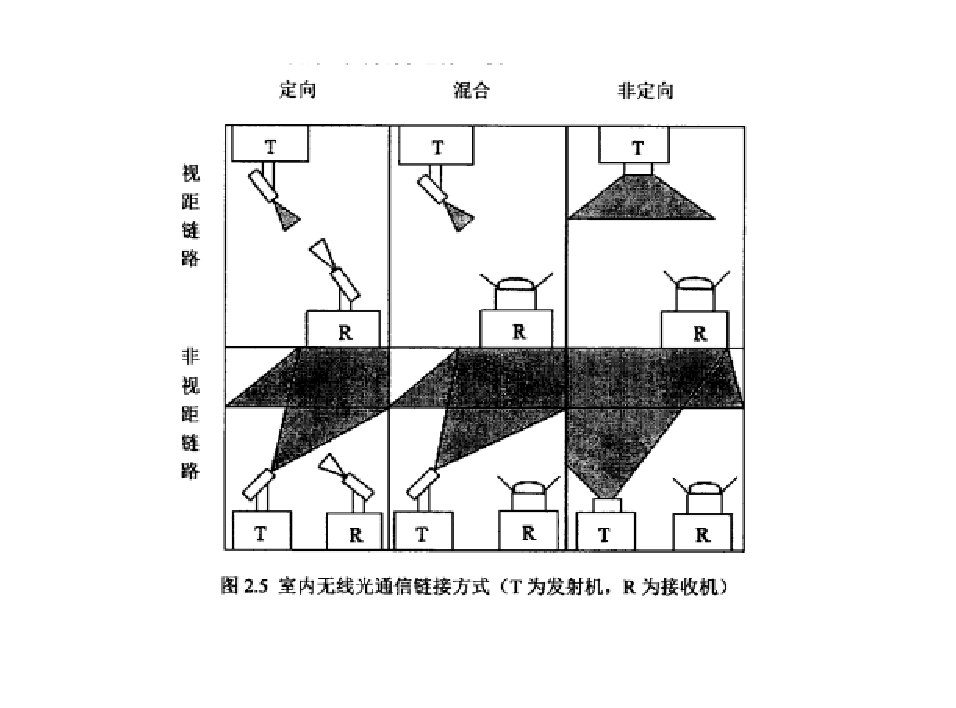
\includegraphics[width=0.8\textwidth]{figures/chapter-2/VlcOnLinkMode.eps}
	\caption{光通信链路划分标准}
	\label{fig:vlc-on-link-mode}
\end{figure}

对于使用可见光作为通信媒介的光通信来说,一般LED灯组都是安放在房间内的天花板上,而用户则处于房间内进行活动。
因此,一般意义上的可见光通信都采用的是视距链路方式。下面主要分析一下在视距链路下的三种不同的链路情况。

首先,考虑的是定向视距链路,使用这种链路类型的系统,为了保证通信的进行,要求发射端和接收端是对准的,由于发射端发出的光散射消耗的光功率较小,
同时接收端的视角又正好集中在发射方向的正对方向,因此这种情况下接收端获得的光接收功率会非常大,同时多径干扰也会非常的小。
但是采用这种方式,要求发射端和接收端要严格对准,一旦接收角度发生一定的变化,或者是链路收到其他障碍物的干扰,都会使得通信的质量大大下降。
同时,这种方式对于用户的移动性的支持也较差,所以它比较适合用于静态的点对点通信的场合中。

其次,可以考虑混合视距链路,对于该链路可以分为两种情况,一种是光发射机的发射角度很大,而光接收机的接收角度较小。另一种是光发射机的发射角度较小,而光接收机的接收角度很大。
对于第一种情况,虽然光发射机发射角度的增加使得接收端获得接收功率下降了,但是也同时提高了发射端光通信可以覆盖的范围,使得用户可以一定范围内运动下仍能保证和灯组进行通信。
而由于接收端的接收角度较小,使得接收端的多径干扰也大大降低,因此这是一种比较实用的光通信链路情形。而对于第二种情况,由于发送端的信号较为集中,而接收端的接收角度较大,这种方式下接收端产生的码间干扰和噪声干扰将会较大。

最后,对于非定向的视距链路而言,增大了发射角度和接收角度,同样这种方式可以对用户的移动性起到有利的影响,使得用户在较大的范围内可以获得灯组的发射信号。但是角度的增加也会带来多径干扰的增强,从而影响链路的通信质量。

在实际的光通信系统中,通常采用混合视距链路中的第一种情况或者是非定向的视距链路进行数据通信。由于在一般情况下,LED灯组的发射角度和灯组的类型有关系,在选定灯组后,该值也就确定了,所以可以研究接收端接收角度的变化对于系统产生的影响,
并选择合适的接收角度进行数据传输。

\subsection{可可见光通信信道分析}\label{sec:vlc-channel}
由上述的分析可知,一般的可见光通信系统采用的是视距链路进行通信。对于视距链路下的通信信道,可以对其信道模型进行详细的分析。对于可见光通信系统而言,可以将其视为一个线性时不变系统[33],该信道模型可以表示为:

\begin{equation}
    y(t) = \gamma \times (x(t) \otimes h(t)) + n(t)
    \label{equ:baseband-channel}
\end{equation}

其中,$y(t)$表示的是接收的电信号,$x(t)$表示的是发送的电信号,$h(t)$是系统的冲击响应,$\gamma$是接收端的检测灵敏度,$n(t)$为系统的加性高斯白噪声,$\otimes$表示卷积。

那么该信道的基本特征也就可以使用该系统的冲击响应$h(t)$来进行描述。这里,首先可以建立可见光通信系统通信时的几何模型,假设其通信时的平面位置图如\autoref{fig:vlc-ji-he}所示。

\begin{figure}[htbp]
    \centering
	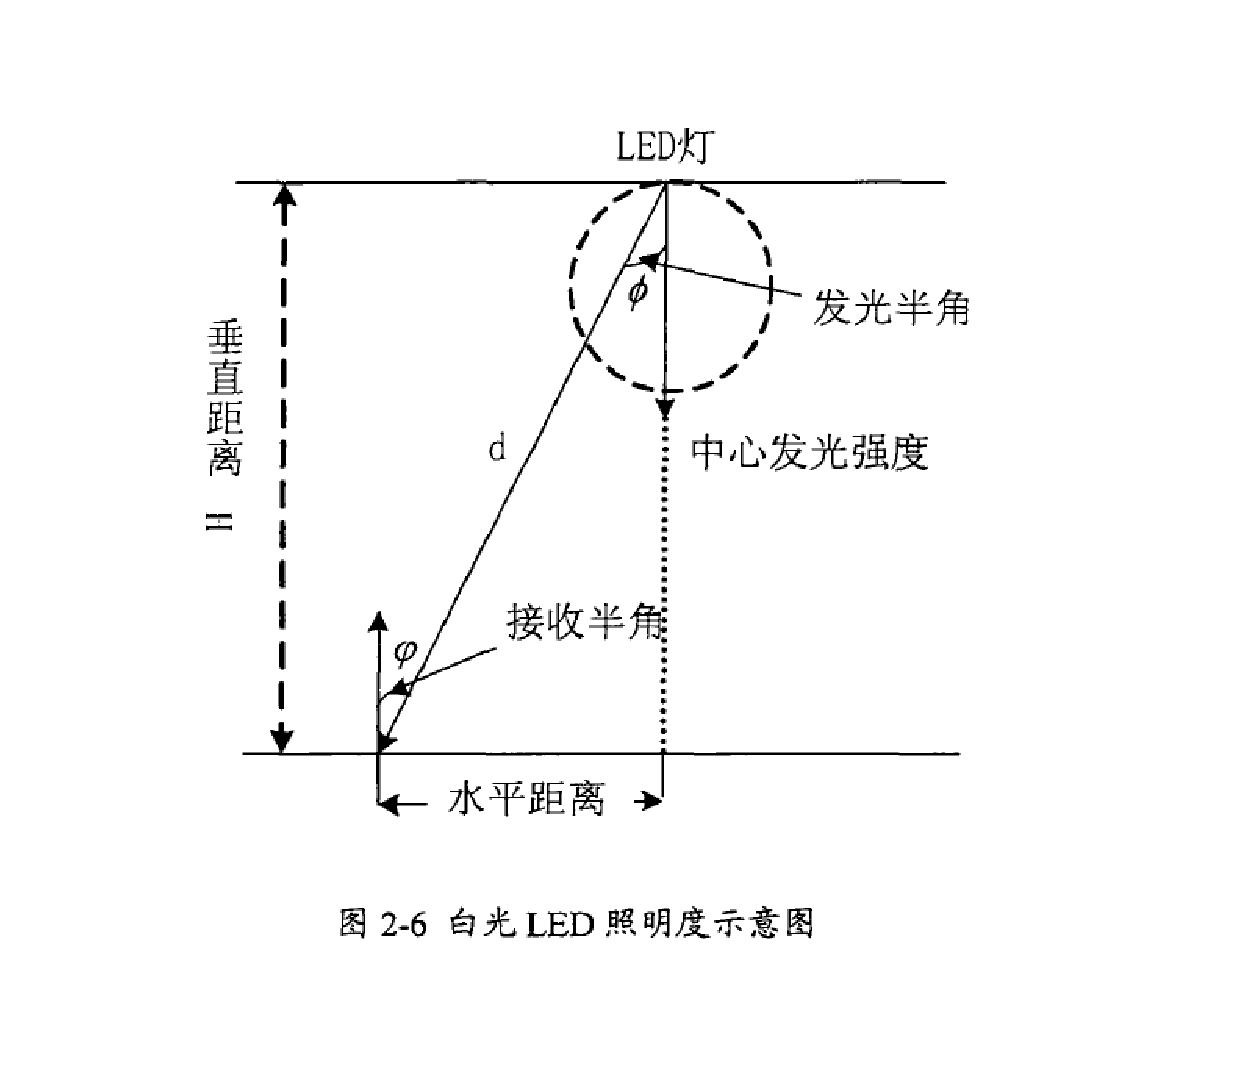
\includegraphics[width=0.8\textwidth]{figures/chapter-2/VlcJiHe.eps}
	\caption{光通信时的平面位置图}
	\label{fig:vlc-ji-he}
\end{figure}

假设发射端特征记为$S$,接收端特征记为$R$,环境特征记为$E$,当使用强度调制/直接检测的方式(Intensity Modulation / Direct Detection, IM/DD)进行通信时,系统的冲击响应可以表示为[34]:

\begin{equation}
    h_{E}(t;S,R) = \sum_{k=0}^\infty h_{E}^k(t;S,R)
\end{equation}

其中,$h_{E}^k(t)$表示的是在环境特征为E的条件下系统对第k条反射链路的冲击响应。假设系统发射端的光源采用朗伯辐射模型,如图\autoref{fig:lambo}所示,图中的$n$表示白光光束的方向性,该值越大,说明光源的方向性也就越好。

\begin{figure}[htbp]
    \centering
	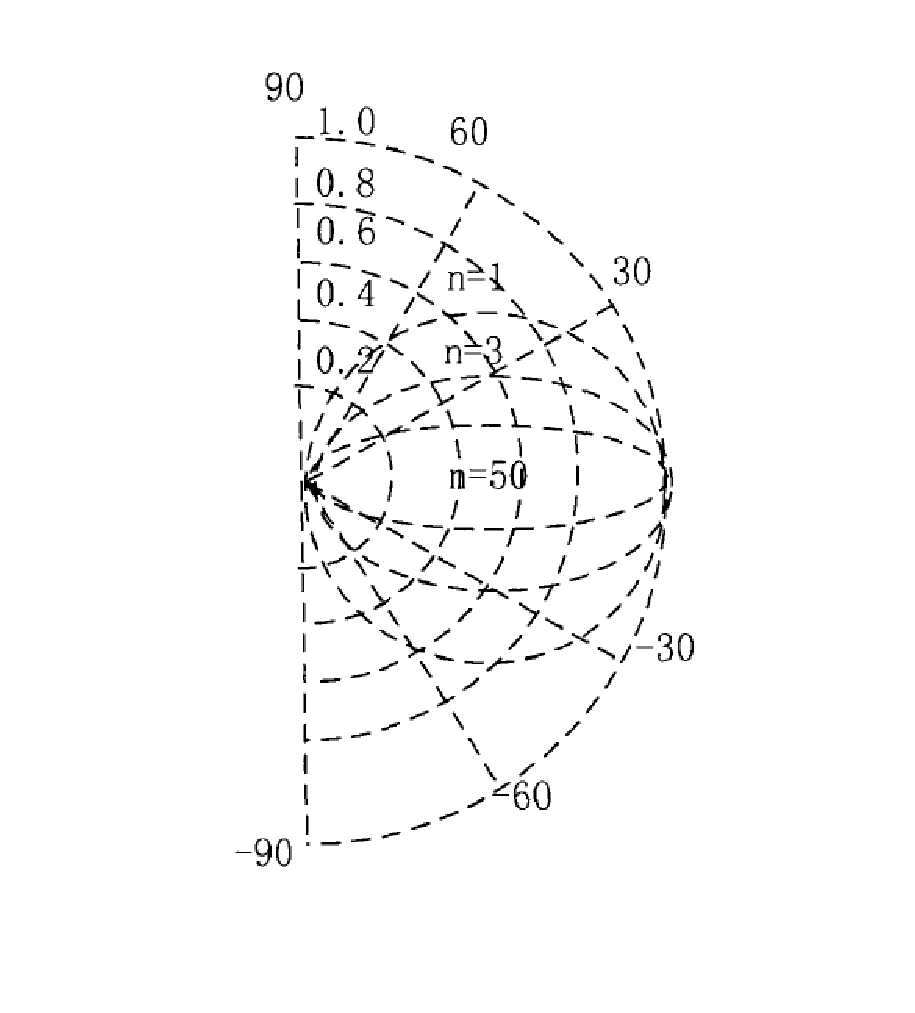
\includegraphics[width=0.7\textwidth]{figures/chapter-2/Lambo.eps}
	\caption{朗伯辐射模型}
	\label{fig:lambo}
\end{figure}

所以光源的辐射强度可以表示为:

\begin{equation}
    T(\phi) = \frac{m+1}{2\pi}\cos^m(\phi),\;\phi\in[-\frac{\pi}{2},\frac{\pi}{2}]
\end{equation}

其中,$m$为朗伯辐射系数,该值和光源的半功率强度有关,$\phi$为接收的角度值。

该模型下系统的发射端特征可以由光源位置$r_{S}$,单位方向向量$n_{S}$和上述的朗伯辐射系数这三元组来确定,即

\begin{equation}
    S=\left\{r_{S},n_{S},m\right\}
\end{equation}

同样,接收端的特征也可以用接收端位置向量$r_{R}$,单位方向向量$n_{R}$,接收端面积$A_{R}$和接收视场角$FOV$这四元组来进行表示

\begin{equation}
    S=\left\{r_{R},n_{R},A_{R},FOV\right\}
\end{equation}

在计算系统的脉冲响应时,通常先观察零次反射的响应函数,即从发射端通过直达径达到接收端时的响应,表示如下[35]

\begin{equation}
    h_{E}^0(t;S,R)=V(E)T(\varphi)(\frac{A_{r}g_{a}(\theta)}{D^2})\delta(t-\frac{D}{c})
\end{equation}

其中$V(E)$表示的在环境特征$E$的条件下的可视函数,如果直达路径上是没有遮挡的,那么该值为1,否则该值为0。$T(\varphi)$是指采用的辐射模型,
$A_{r}$是光接收面积,$D$是源端和接收端之间的距离, $g_{a}(theta)$是接收器的增益函数,可以表示为

\begin{equation}
    g_{a}(\theta)=
    \begin{cases}
        1,  & \theta\le\psi_{c} \\
        0,  & \theta>\psi_{c}
    \end{cases}
\end{equation}

其中,$\theta$为接收端的入射角,$\Psi_{c}$为接收端的视场角。

当获得了$k$-1次反射响应函数之后,就可以通过迭代的方式求出第$k$次反射的响应函数[36]:

\begin{equation}
    h_{E}^k(t;S,R)=\int_{S} \rho_{r}h_{E}^{k-1}(t;\{r,n,1\},R)\otimes h_{E}^0(t;S,\{r,n,\frac{\pi}{2}, \, dr^2\})
\end{equation}

上述意味着在环境特征为$E$的条件下,对于接收端的表面进行积分。$r$是$S$中的微反射体的位置向量,$\rho_{r}$是$r$处微反射面的发射系数,$n$是$r$处微反射面的单位法向量。

这样通过式(2-5)和式(2-7),可以得到接收端的任意第k次的发射响应函数。
而在实际情况下,并不需要考虑无穷次的发射链路的冲击响应,因为随着反射次数的增加,对应的冲击响应的能量值也越来越小,
所以在计算总的冲击响应时,只需要考虑前M次的反射的冲击响应即可,所以总的冲击响应的表达式可以如下表示

\begin{equation}
    h_{E}(t;S,R)\approx \sum_{k=0}^M h_{E}^k(t;S,R)
\end{equation}

一般情况下,M取3即可表现出整体的冲击响应[37]。因此,通过上式,就可以求出室内可见光通信系统中的总的冲击响应表达式。

在室内可见光通信系统中,若只考虑直达路径,接收端的光接收功率可以表示为

\begin{equation}
    P_{r}=H_{E}(0;S,R)P_{t}
\end{equation}

其中,$P_{t}$为发射端的光发射功率,$H_{E}(0;S,R)$为信道的直流增益。该值则可以通过系统的冲击响应积分计算得到,即

\begin{equation}
    H_{E}(0;S,R)=\int_{-infty}^{+infty} h_{E}(0;S,R)\, dt
\end{equation}

将上述的式(2-8)代入式(2-10)后,可以得到直流增益的表达式为

\begin{equation}
    H_{E}(0;S,R)=
    \begin{cases}
        \frac{(m+1)A}{2\pi D_{d}^2}\cos^m(\phi)T_{s}(\psi)g(\psi)\cos(\psi),  & 0\le\psi\le\psi_{c} \\
        0,  & \psi>\psi_{c}
    \end{cases}
\end{equation}

其中,$\phi$是发射信号出射角,$\psi$是接收信号入射角,$m$是朗伯系数,$A$是接收端的探测面积,$D_{d}$是灯组和用户之间的距离,$T_{s}(\psi)$是光滤波器的增益值, $\psi_{c}$是接收端的视场角。$g(\psi)$是光接收器的增益,可以表示为

\begin{equation}
    g(\psi)=
    \begin{cases}
        \frac{n^2}{\sin^2\psi},  & 0\le\psi\le\psi_{c} \\
        0,  & \psi>\psi_{c}
    \end{cases}
\end{equation}

另外,还需要考虑此时的系统接收信噪比。假设发射端发射的信号为 ,接收端收到的电信号功率可以表示为

\begin{equation}
    S=\gamma^2P_{rSig}^2
\end{equation}

其中$\gamma$表示的是接收端的光电转换效率,而$P_{rSig}$则是在单位时间内接收到的信号的功率,可以表示为

\begin{equation}
    P_{rSig}=\int_{0}^{T} h(t) \otimes x(t)\, dt
\end{equation}

而在室内光通信条件下,接收端的噪声主要由三部分组成,即为散粒噪声,热噪声和码间干扰噪声[38],所以总的系统噪声可以表示成

\begin{equation}
    N=\sigma_{shot}^2+\sigma_{thermal}^{2}+\gamma^2P_{rISI}^2
\end{equation}

其中各部分的噪声也可以分别表示为[39]:

\begin{equation}
    \sigma_{shot}^2=2q\gamma(P_{rSig}+P_{rISI})B+2qI_{bg}I_{2}B
\end{equation}

\begin{equation}
    \sigma_{thermal}^2=\frac{8\pi kT_{k}}{G}\eta AI_{2}B^2+\frac{16\pi^2kT_{k}\Gamma}{g_{m}}\eta^2A^2I_{3}B^3
\end{equation}

\begin{equation}
    P_{rISI}=\int_{T}^{\infty}h(t) \otimes x(t)\, dt
\end{equation}

其中,$q$为电子的带电量,$B$为接收电路的等效噪声带宽,$k$为玻尔兹曼常数,$T_{k}$为绝对温度,$\eta$指探测器单位面积上的电容,$I_{bg}$为背景电流,$I_{2}$为噪声带宽因子,$G$为开环电压增益,$\Gamma$为FET噪声因子,$g_{m}$ 为FET的跨导,$I_{3}$为常数[]。

因此,接收端的接收信噪比SNR也就可以通过下式计算得到

\begin{equation}
    SNR=\frac{P_{rSig}}{N}
\end{equation}

根据上述理论分析,可以计算出系统接收的信噪比。同时,上述的分析也展示了影响接收端信噪比的两个重要方面。首先,在上述计算信噪比的过程中,采用的是总的系统冲击响应,
但是在实际的过程中,根据文献[40]的描述,在室内可见光通信系统中,通过墙面等反射体的发射到达接收平面的信号能量要远小于通过直达径到达的信号能量,因此在实际仿真中计算接收端的信噪比时,
在信号功率的计算方面,可以只计算直达径获得的信号能量,忽略通过发射到达接收端的信号能量。其次,由于信噪比中的噪声除了受系统的热噪声等不可抗拒因素影响以外,还很大程度上取决于系统接收端的码间干扰。
而接收端码间干扰的形成则是由于发送端的信号经过多个不同的光路径达到接收端。这里的发送端的光信号可能既来自目的灯组,也来自目的灯组以外而定其他不同的光源。
所以,当我们在设置室内的LED灯组布局时,既要考虑到通过增加LED灯组的个数,减小接收平面的"阴影"区域,同时还需要注意多个LED灯组的重叠覆盖导致的用户接收端的多径效应[41]。

\section{通信系统组网技术研究}\label{sec:network-tech-researh}
\subsection{相关系统的组网方案}
在移动通信领域,对于组网技术的研究也一直是一个热门的问题。对于移动通信网的组网的定义,一般是以增加系统的效益作为目标,采用各种通信技术和设备来有效地组织、管理和调度网络。

在目前推出的准4G标准LTE中,使用了六类组网技术来克服系统对于上下行组网时遇到的挑战,文献[42]对LTE系统中的组网技术进行了较为完善的总结,
其将LTE中的组网技术归纳为以下6点:时域与频域调度、跳频、码分复用、空间波束赋形、功率控制和接收机算法增强。其中,时域与频域调度是为了抑制小区内部的干扰,采用对时域和频域资源的合理调度,
达到多用户的无干扰数据传输。调频技术则是在上述的数据传输中,对于同一用户在不同的时刻采用不同的频率进行传输。LTE中的码分复用是体现在两个方面,一个是加扰,另一个是扩频,
加扰是使用一定的随机序列对小区发送的数据进行扰乱,从而使得干扰随机化,来抑制小区间的干扰。而扩频则是利用无关的码来对被传输信号进行频谱扩展,从而有效抑制干扰。空间波束赋形则是通过对多天线阵列的控制,
使得发送出去的信号呈现一定的方向性,从而可以根据用户的位置,发射信号时选择正确的方向,并抑制用户之间的干扰。由于LTE系统使用的是同频覆盖,因此功率控制的目的是指通过对系统中的资源进行合理的管理,
从而协调好多个小区之间的动作,从而避免产生严重的小区间干扰。接收机算法增强也是指干扰删除,包括基于多天线的空间干扰压制技术和基于干扰重构的干扰消除技术。上述组网技术保证了在LTE系统中对基站间的相互干扰取得有效地控制,
从而获得整个网络的更高的吞吐量。

而作为室内无线通信最常使用的无线局域网技术,其组网方式通常可以分为两种类型,对等网络和基础结构网络[43]。其中对等网络,是指由一组具有无线接口的计算机组成的网络,网络中的任意两台机器都可以进行直接通信。
而在基础结构网络中,使用了无线接入点将无线局域网和有线网连接起来,在无线局域网中,各节点通过接入点进行相互通信。对于广泛使用的基础结构网络中,又分别提出了胖接入点(Fat AP)技术和瘦接入点(Fit AP)技术[44],并根据实际的场景进行定制。胖接入点技术将无线局域网中的物理层,数据加密,用户认证,网络管理,漫游技术和应用层技术结合起来,
使得每个胖接入点都可以成为一个独立和有线网连接的个体。但是胖接入点只能进行单独配置,且所有的软件都要保存在接入点上,在大型网络下对于接入点的管理和维护工作量大。
因此,瘦接入点技术被提出。瘦接入点只完成无线局域网中的物理层的工作,而其他的功能,如用户认证,安全管理,网络管理和应用层功能都被上移到接入控制器(AC)上进行。
这样的好处就是在进行大规模组网的时候,只需要对接入控制器进行配置,部署便捷,同时此类系统还可以支持快速切换,并可以进行有效的网络安全管理和控制。

\subsection{室内光通信系统组网的问题}
上述提及的是移动蜂窝网和局域网中常用的组网方式,而在室内可见光通信系统中,考虑到可见光通信的技术特点和典型的组网架构,组网中的关键技术主要包括可见光光源布局研究,可见光网络切换技术,
可见光网络接入控制技术,系统级的资源分配方案等一系列的内容[45]。

其中,可见光的光源布局是指采用合理的光源布局,来满足可见光通信系统的照明和照明的需求。在常见的光通信应用场景中,通常使用多个灯组进行室内有效地覆盖,作为通信设备使用的灯组,
其布局情况必定对整个系统的性能有着重要的影响。对于光源的布局设计,需要考虑到房间的大小,灯组的选择,直射距离等信息,从而对LED间隔的大小,排列和位置,LED灯组的个数等信息进行合理的设计,从而保证系统的通信性能。

可见光网络切换技术则是为了支持室内用户的移动性,当用户在室内随意走动时,仍能保证用户和灯组之前的可靠链路通信。这是因为光通信的一个显著特点就是信号的衰减较快,因此每个灯组的覆盖面积较小,
当用户进行了移动后,很有可能就会从一个灯组的覆盖区域移动到另外一个灯组的覆盖区域,所以,灯组之间的垂直或是水平切换策略就显得特别重要。类似于蜂窝通信系统,在可见光通信系统中一般会对某用户的当前服务灯组的信号质量进行跟踪,
当发现当前的服务灯组的信号差到一定的程度时,就需要寻找新的可接入灯组并选择合适的接入方式进行接入。

可见光网络接入控制技术则是为了在有下行干扰的条件下,进行上行接入的控制技术。由于在进行灯组组网时,接收平面是很多地方是多个灯组的重叠覆盖区域,因此,当用户处于这些位置时,就会存在较为严重的相邻灯组下行干扰,
如果用户上行传输仍然是采用光通信的话,就必须使用某种接入控制技术,例如采用基于角度感知的定向接入协议,来保证干扰下用户上行通信的进行。

系统级的资源分配方案则是针对于当前的灯组布局和用户的情况,采用合适的灯组调度策略,减小系统中用户之前的干扰,并实现系统吞吐量的最大化。
在不同的光通信系统中,灯组的控制方式也可以是不一样的,就如上述的局域网系统而言,如果所有的灯组的控制功能如用户鉴权,加密,漫游控制等全部由连接各灯组的控制中心负责,
各个灯组可以看作是一个单纯负责物理层通信的实体,那么这种控制方式可以被称为分布式灯组控制,而如果所有的灯组都具有对其覆盖范围内的用户具有控制功能,每个灯组可以进行独立的配置,
那么这种控制方式可以称为独立式灯组控制。针对这两种情况,可以分别进行研究,讨论需要采用何种的调度策略进行系统资源的分配,从而保证多用户的光通信系统可以获得较大的系统容量。

上述这些组网技术将会保证可见光通信系统可以更加高效地使用资源,更加灵活地配置和管理网络,对光通信系统的实际的运行具有重要的意义。在本文的后续章节中,鉴于本文的承载量,本文将会对上述组网技术中的部分内容进行研究和分析。

\section{本章小结}
本章主要介绍了可见光通信系统的基础理论,为之后章节的具体分析奠定了理论基础。
首先,介绍了室内可见光通信和传统的室内光通信(以红外通信为例)的区别,并通过比较可以了解到室内可见光通信在频谱资源,安全性,适用范围等方面的显著优势。
这也是可见光通信将会代替目前的室内光通信技术的一个重要依据。
接着,本章介绍了室内光通信的链路方式的划分标准,并指出了常见的可见光通信的链路方式,
以此为基础,本章介绍了可见光通信的信道模型,并对接收端的信噪比等典型参数进行了理论分析。
最后,本章还重点对于研究的组网领域进行了介绍。主要介绍了常见的通信系统,如移动蜂窝系统和室内局域网系统中目前常用的组网技术,
同时介绍了可见光通信系统在组网方面需要解决的关键技术问题,为后续的本文研究指明了研究的方向。

    % !Mode:: "TeX:UTF-8"
% 光信道建模:线性信道(小信号)与非线性(大信号)信道模型

\chapter{室内可见光通信系统灯组布局优化}\label{chap:led-layout}
\section{引言}
在可见光通信系统中,灯组必须兼具室内照明和数据通信两大功能,而室内可见光通信系统通常是由多个灯组组成的,因此对于灯组分布的优化就成为了一个重要的问题。
不同的灯组的分布,对应着不同的光照强度和不同的光接收功率分布。从文献[]中可以知道,合适的室内灯组分布,需要能够尽量使得光照强度和光接收功率均匀化。
同时,为了满足数据通信的基本要求,合适的灯组布局还需要尽可能地提高平均光接收功率强度,以满足高速的数据通信需求。
同时,在考虑LED灯组的安置问题的同时,由于系统使用的LED灯组通常是由多个LED灯组成的,因此还需要考虑灯组内的LED等应该如何组织这个问题。
在本章中,将会首先分析系统采用的可见光通信灯组的模型,并在此模型的基础上,提出了针对于光照强度和光接收功率这两个指标进行优化的灯组分布优化方案,
并给出了优化的仿真结果和光照强度分布和光接收功率分布曲线,以检验灯组布局优化的效果。

\section{可见光通信灯组模型}\label{sec:led-model}
\subsection{白光LED特性介绍}
LED是一种能够发光的半导体的电子元器件,其早期出现时只能发低光度的红光,后来在不断地研究中,出现了白光发光二极管,发光度也得到了很大的提升,从而使得白光二极管被应用于家用的照明中。
发光二极管只能够在一个方向导通,叫做正向偏置,当电流流过时,电子与空穴在其内重合而发出单色光,这叫电致发光效应[47]。
由于白色LED转化效率高,反应快,可靠性强,环保等特点,且其使用的成本已经大大低于目前的常用灯源,所以白光LED已经开始大范围地应用于家庭照明中。

LED的发展可以概括为由单一光向白光的转变,由低效率向高效率的转变。
在1961年,美国德州仪器公司的研究人员首次发现砷化镓等半导体合金会进行红外放射作用。
并于次年,有美国通用电气公司的研究人员开发出了可以被使用的可见光二极管。
在1993年,日本的中村修二利用镁掺入,发明了高亮度的蓝色发光二极管,并因此获得了2014年的诺贝尔物理学奖,以表彰其在白色环保能源方面的重要贡献。
在蓝色发光二极管被发明之后,白色发光二极管也随即问世,为室内的照明提供了基础。
但是当前的LED的发光强度仍然较低,在之后的20年中,为了制作出更加实用的LED灯,各大企业和研究机构不断投入资金,提高LED等的光照性能。
其中,日本的发光二极管厂商日亚化工和美国发光二极管厂商科锐不断地刷新LED的光效记录。在2012年4月,美国科瑞公司的LED光效已经能到达到254 lm/w。

常见的白光LED发光的方式按照发光二极管数量的不同可以分为单晶体和多晶体两种类型[48]。多晶体是指采用互补的LED发光二极管或者是将蓝红绿三种颜色的发光二极管组合在一起,混合之后产生白光。
这种方式发成的白光色域较宽,同时比其他方式的效率高,但同时生产成本也较高。另外一种正被大规模采用的LED生产方式就是采用单晶体方式,单晶体是指首先使用某一单元发出单一颜色波长较短的光,
比如蓝光或者是紫光,再使用磷光剂将短波长的光转化成长波长的白光。由于在转化过程中部分能量转化为热能,会造成能量的消耗,所以这种方式产生白光的发光二极管效率较低。

传统的照明,比如说荧光灯,白炽灯等,是装载有气体的玻璃管的形式,因此并不如被称为固态照明的发光二极管实用。
由于当增加二极管的光度时,二极管的效率也会下降,所以对于需要使用LED获得高亮度的情况,一般都是采用多个小的LED灯组成成为一个LED光源,而对于一些对光度要求低的场合,
单个的LED等也可以被直接使用来满足照明需求。

在1967年法国举行的第十三届国际计量大会上,``坎德拉'',``坎德拉/平方米'',``流明'',``勒克斯''被分别作为发光强度,光亮度,光通量和光照度的单位,作为照明领域最常用的几个量度。
其中光强度是指光源在指定方向的单位立体角内发出的光通量。绝对黑体在铂的凝固温度下,从5.305*10cm面积上辐射出来的光通量被定义为1lm。光亮度指发光表面在指定方向上的发光强度与垂直于指定方向的发光面积之比。
而光照度的定义为,被光均匀照射的物体,在1平方米面积上得到的光通量是1流明时,它的照度就是1勒克斯。

\subsection{室内LED灯组结构}
本章中将研究典型的室内光通信场景模型,并以此为基础进行灯组分布的优化。以一般的光通信应用场景,如办公室或者是会议室为例,本章设置了一个5*5*3的房间模型。
在该房间中安装有四个LED灯组,每个灯组被安放在距离地面2.5米的位置,房间中运动的用户的手持接收终端假定都处于1米的接收平面上,其灯组在室内的平面示意图如下图所示。

\begin{figure}[htbp]
    \centering
	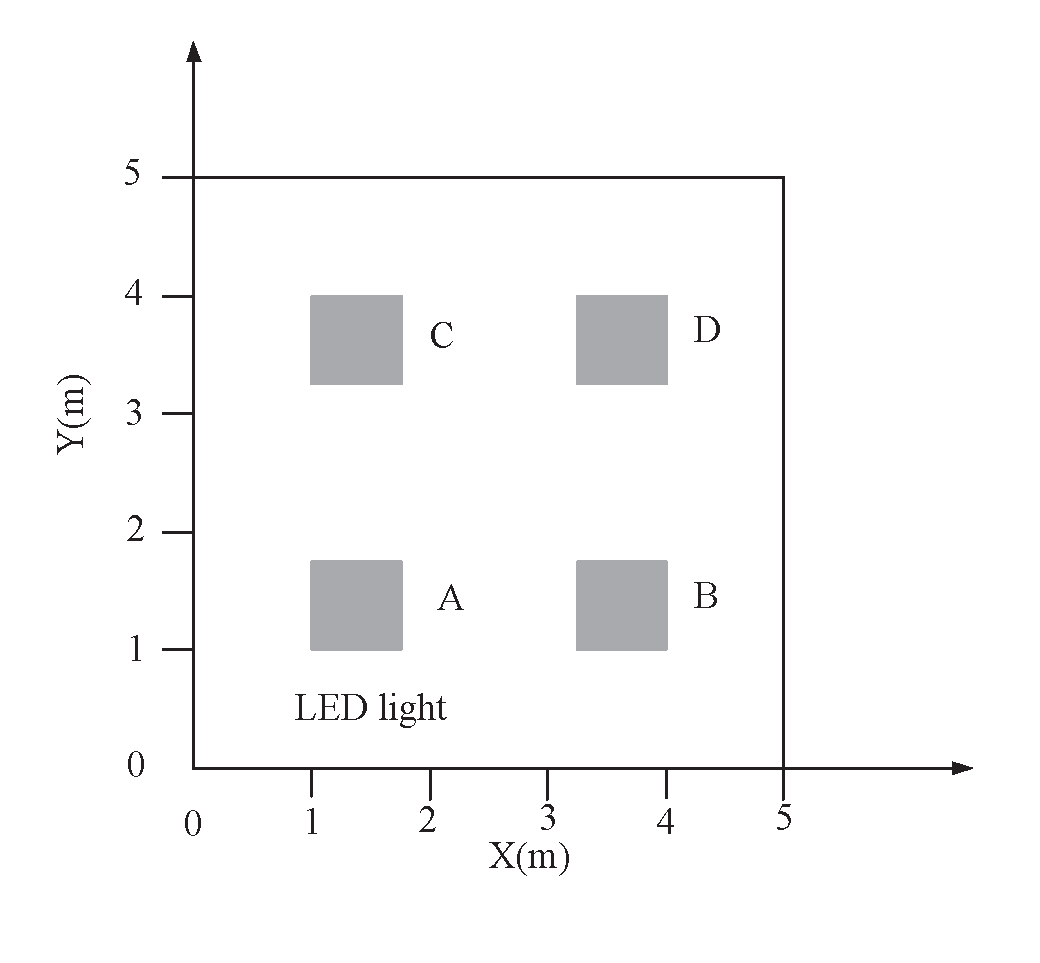
\includegraphics[width=0.8\textwidth]{figures/chapter-3/LedLayout.eps}
	\caption{室内可见光通信灯组分布基本模型}
	\label{fig:led-layout-pic}
\end{figure}

对于发射端而言,为了提高LED灯组的照度和覆盖范围,每个LED灯组都包含有3600(60*60)个LED灯。
对于每一个LED而言,其发射半角是确定的,为70度,其中心的发光强度为0.73cd,中心的发光功率为20毫瓦。
对于用户接收器而言,其接收器探测表面积为1平方厘米,用户接收视场角为60度,光电转化效率为0.53A/W,
光滤波器的增益为1,其所有参数均列表显示如下。

\begin{table}[htbp]
    \caption{光通信灯组布局中使用的参数值}
    \label{tab:led-layout-param}
    \centering
    \begin{tabular}{llll}
        \toprule
        参数 & 取值 & 参数 & 取值\\
        \midrule
        房间长*宽*高     & 5*5*3($m^3$) & 接收视场角          & 60deg. \\
        接收平面高度     & 1m           & 一个灯组包含的LED数 & 60 \\
        LED中心发光强度  & 0.73lm       & 接收端检测面积      & $10^{-4}$ ($m^2$) \\
        LED中心发送功率  & 0.02w        & 光滤波器增益        & 1 \\
        发射机半功率角   & 73deg.       & 光接收器增益        & 3 \\
        光电转换效率     & 0.53         & 接收端折射系数      & 1.5 \\
        \bottomrule
    \end{tabular}
\end{table}

一般来说,在构建一个室内可见光通信系统时,在上述提及的参数后,还需要确定的变量就是灯组在安装平面的位置,以及组成LED灯组的各LED灯之间的间隔。
这两个参数值也将会直接影响到光照分布和光通信系统的通信质量,下文中也将以这两个变量作为优化的参数。

\subsection{灯组分布优化方案}\label{sec:led-layout-design}
为了保证房屋内的照明和高质量通信的要求,需要在上述灯组结构的基础上,对室内灯组的具体位置指标进行设计。首先,需要明确室内灯组布局优化的几个目标。
第一点,设计的灯组的布局应该能使得室内的光照分布和接收光功率分布要尽可能地均匀,从而使得用户在室内照明和数据通信上都可以获得良好的使用体验,
第二点,室内光通信的目标是实现高速短距离的数据通信,灯组的布局优化也应该以此为目标,通过对灯组的布局调整,在用户接收端获得较高的接收功率,
第三点,根据国际标准化组织的规定,办公室内合适的光照强度的范围为300-1800lm,此范围的光照强度会让人感到最为舒适,因此规定的室内光照强度范围必须是灯组布局设计的一个重要依据。
根据上文描述,假定每个LED灯组的发射功率都是一样的,灯组在室内组装时,可以通过优化灯组摆放在房间中的位置和灯组之间的间隔,满足室内照明和通信的需求。

根据上文的分析,灯组布局优化问题可以看作为通过设计几项参数使得设计的目标达到最优的这样一个问题,因此可以采用了一个最优化模型对灯组布局优化问题进行建模。在进行最优化灯组布局建模时,将系统优化的参数用一个向量x来进行表示:

\begin{equation}
    x=\left[d \quad i\right]^T
\end{equation}

其中$d$表示的是灯组距离房间中心点的水平方向上的距离,$i$表示的是灯组之间的距离,如下图所示。

\begin{figure}[htbp]
    \centering
	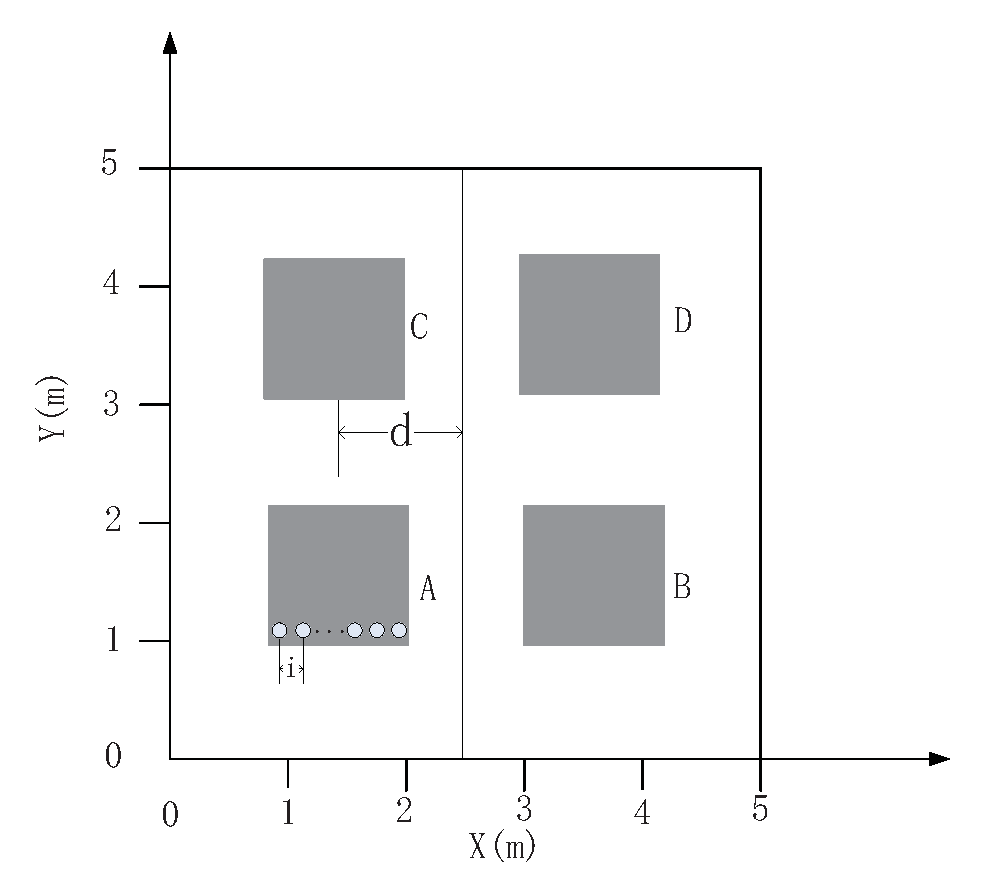
\includegraphics[width=0.8\textwidth]{figures/chapter-3/LedLayoutDI.eps}
	\caption{光通信室内灯组分布参数示意图}
	\label{fig:led-layout-d-i}
\end{figure}

上述需要考虑的目标问题也就成为模型需要考虑到多个优化目标,其中第一点的目标要求最大化模型的光照强度和光接收功率的均匀度,将该目标函数设为$f_{1}(x)$。
第二点的目标要求最大化模型的接收平面的平均光接收功率,将该目标函数设为$f_{2}(x)$,第三点,则可以成为最优化模型的接收条件。
由于第一点和第二点的目标函数是不能同时达到最优的,即系统不太可以在光照强度和光接收功率很均匀的情况下,获得最好的平均光接收功率,因此,本文的最优化模型也就变成了多目标优化的模型,如下式所示。

\begin{equation}
\begin{aligned}
    \max\quad & \left[f_{1}(x) \quad f_{2}(x)\right] \\
    \mbox{s.t.}\quad & 300\le minE_{or}(x) \le maxE_{or}(x) \le 1800 \\
           & 0 \le d \le 2   \\
           & 0 \le i \le 0.04 \\
           & d+\frac{n-1}{2}*i \le L
\end{aligned}
\end{equation}


其中,$E_{or}(x)$表示的是系统灯组参数为$x$的情况下的光照强度分布,$n$表示的是灯组中一排的LED数目值,根据前文中对灯组结构的描述,该值被设置为60,$L$为房间的宽度的一半。

对于上述的各目标函数,需要进行定量地分析。目标一中的均匀度可以分别使用灯组光照分布的方差和光接收功率分布的方差进行衡量,要求计算出的结果是越大越好,
系统的均匀度的目标取决于上述的这两个方差目标,假设灯组在某一灯组布局参数条件下的光照分布的方差为$\delta_{e}(x)$和光接收功率分布的方差为$\delta_{p}(x)$,那么就可以得到这两个方差组合成的在某一灯组布局参数条件下对均匀度目标函数:

\begin{equation}
    f_{1}(x)=-\delta_{e}(x)-\delta_{p}(x)
\end{equation}

另外,需要考虑的还有目标二中的目标函数,这里可以直接采用平均接收功率强度去衡量,同样,假设在某一灯组布局参数条件下的平均光接收功率为$\overline{P}_{or}(x)$,那么目标二的目标函数为

\begin{equation}
    f_{2}(x)=\overline{P}_{or}(x)
\end{equation}

因此要优化的目标函数则变为

\begin{equation}
    max \left[-\delta_{e}(x)-\delta_{p}(x)\quad \overline{P}_{or}(x) \right]
\end{equation}

对于该复杂的多目标优化问题,本文采用统一目标函数法将该问题转变为单一目标的最优化函数来进行简化,这里采用较简单的线性加权法来进行处理,线性加权组合法的基本思想就是在多目标最优化问题上,
将其各个分目标函数根据其数量级和在整体优化设计中的重要程度相应地给出一组加权因子,再进行线性组合,从而构成一个新的统一单目标函数。

同时,由于本模型中的两个目标函数都是具有单位的,因此不能被直接进行线性加权使用,因此,首先需要对均匀度和平均光接收功率这两个目标函数值进行归一化,本文中两个目标函数都按照如下的归一化方法进行

\begin{equation}
    \overline {f(x)}  = \frac{{f(x) - \min f(x)}}{{\max f(x) - \min f(x)}}
\end{equation}

归一化后的数据值都将变为0和1之间。

由于本文中的目标函数个数为2,因此,只需要假设一个参数因子$\alpha$,处理后得到的新的目标函数为

\begin{equation}
    \max f(x) = \alpha  \times \overline {{f_1}(x)}  + (1 - \alpha ) \times \overline {{f_2}(x)}
\end{equation}

其中,$\overline {{f_1}(x)}$和$\overline {{f_2}(x)}$分别表示归一化后的目标函数一和目标函数二。

于是,该优化问题就转变为一个多个约束条件下的单目标优化问题,同时对于$\alpha$的值,可以灵活地调节,在趋向于分布均匀的室内光强和光功率和趋向于更高平均接收功率的光强分布之前进行平衡,以获得所期待的光照强度和光功率分布结果。

\section{仿真实验及结果分析}\label{sec:led-layout-simulation-result}
上根据上述的理论分析,本文通过Matlab软件建立了室内可见光通信模型,并按照上述的最优化模型在约束范围内搜索使得目标函数达到最大的灯组最优分布结果。
在结果展示中,分别通过计算室内的光接收功率分布和光照强度分布来描述模型优化对室内照明和通信质量这两方面的影响。

根据上文中模型的描述,模型参数 决定的是系统在均匀度和光接收功率这两个目标上的分别的权重,所以我们可以通过改变 的值,来考察模型在不同的均匀度和接收功率需求下的灯组的最佳分布。

\subsection{偏重平均光接收功率的最佳灯组布局}
为了查看系统在高光接收功率需求下的优化结果,令模型中 取值为0.1,也就意味着在统一评价目标更加看重于平均光功率这一目标,此时,模型搜索出来的灯组放置结果为:$d = 1.2$,$i = 0.015$。

仿真得到的光功率分布图和光照强度分布图如下所示。

\begin{figure}[htbp]
    \centering
	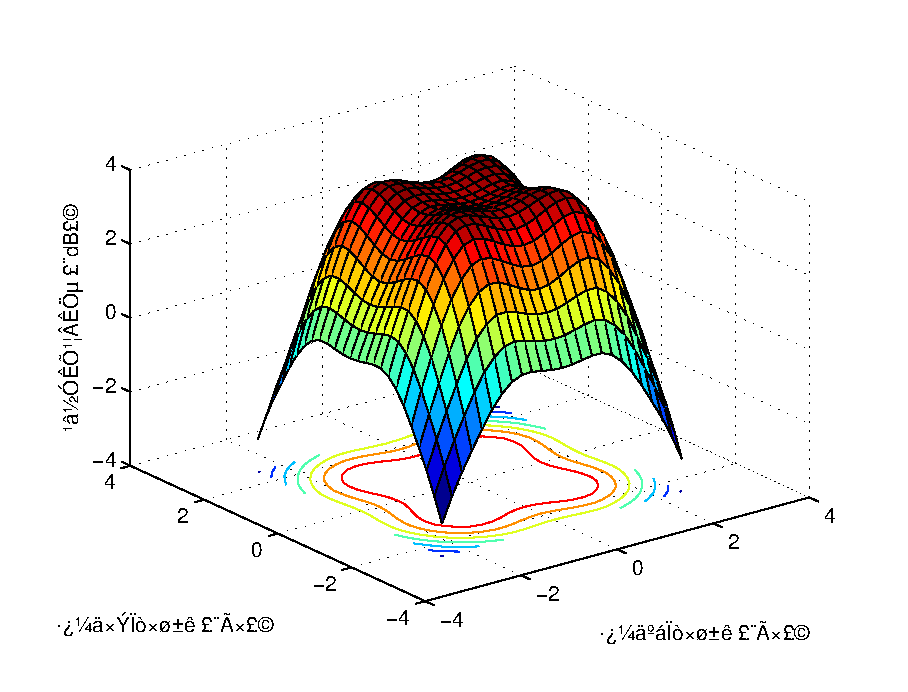
\includegraphics[width=0.7\textwidth]{figures/chapter-3/PowerFirstPower.eps}
	\caption{偏重平均光接收功率时的光接收功率分布}
	\label{fig:power_first_power}
\end{figure}

\begin{figure}[htbp]
    \centering
	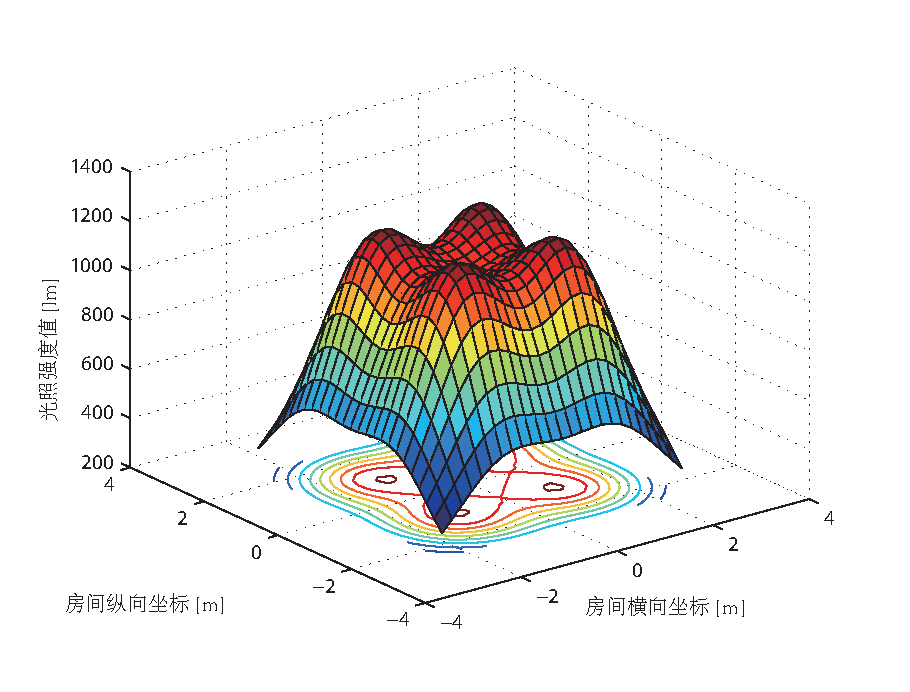
\includegraphics[width=0.7\textwidth]{figures/chapter-3/PowerFirstIllu.eps}
	\caption{偏重平均光接收功率时的光照强度分布}
	\label{fig:power_first_illu}
\end{figure}

从上图中可以看到,当对系统的光接收功率要求较高时,此时优化后的灯组将会被放置在更靠房屋中心的位置,且四个灯组的放置都较为集中,使用在房屋中心区域的光接收功率较高,
然后向外依次递减,此时,光功率最大值为3.9932dBm,最小值为-3.1157dBm,平均值为1.9982dBm。光照强度最大值为1213lm,最小值为301lm,平均值为857lm。

在这种灯组布局情况下,室内中心区域的光照强度较高,光接收功率值也较高,用户可以再室内中心区域获得很好的通信质量和照明效果,但是其对边缘区的覆盖不足,
会导致当用户运动到室内的边缘区域后,其光通信的质量会出现迅速的下降,照明效果也远差于中心区域。

\subsection{偏重整体均匀度的最佳灯组布局}
同时,为了研究系统在对整体均匀度要求较高时的灯组优化布局情况,我们可以将模型中的 设置为0.9,在计算系统评价函数时更加看重于光照强度和光功率的均匀度,同
样对设定的可行域进行搜索之后,通过仿真可以获得灯组的最优分布为$d = 1.7$,$i = 0.025$。

在该情况下得到的最优光功率分布和光照强度分布分别为

\begin{figure}[htbp]
    \centering
	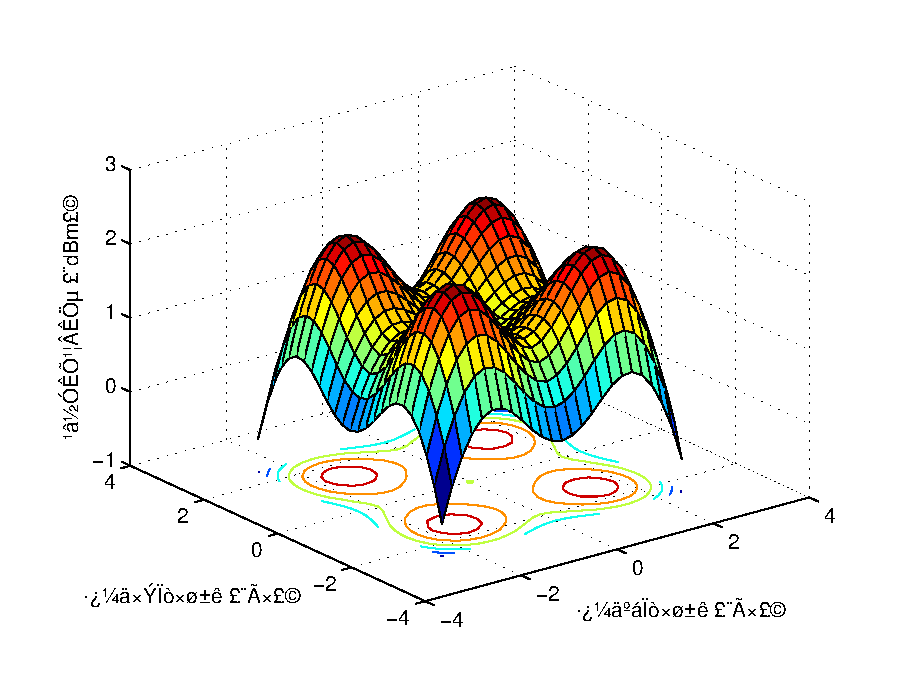
\includegraphics[width=0.7\textwidth]{figures/chapter-3/BalanceFirstPower.eps}
	\caption{偏重整体均匀度时的光接收功率分布}
	\label{fig:balance_first_power}
\end{figure}

\begin{figure}[htbp]
    \centering
	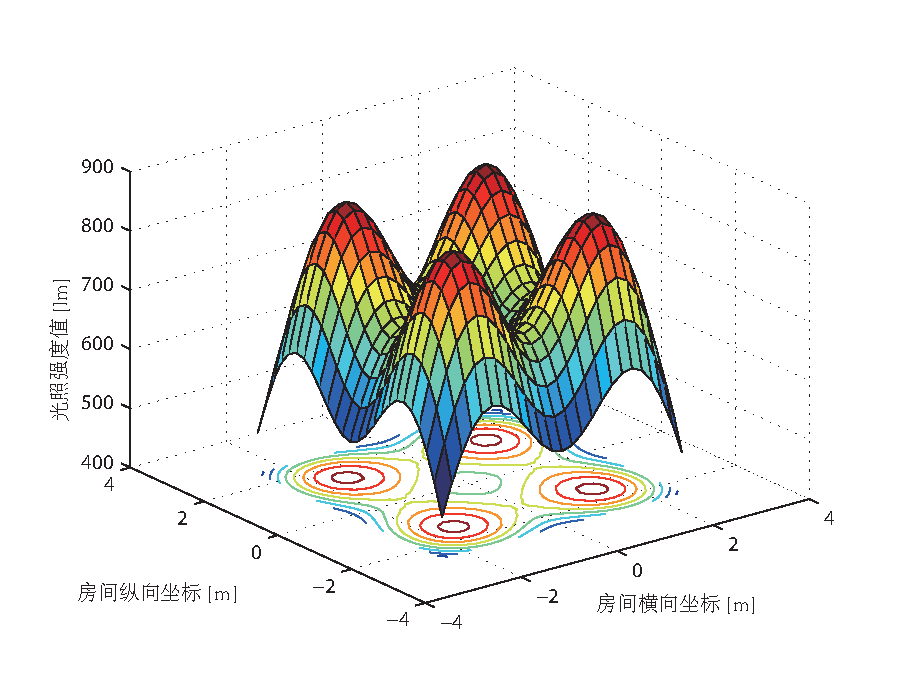
\includegraphics[width=0.7\textwidth]{figures/chapter-3/BalanceFirstIllu.eps}
	\caption{偏重整体均匀度时的光照强度分布}
	\label{fig:balance_first_illu}
\end{figure}

根据上图,当模型对系统的均匀度要求比较高时,灯组在室内的布局将会更加分散,同时灯组之间的距离也会相应地拉大,以保证系统指标的更可能的均匀化。仿真得到的光照强度和光接收功率值的变化范围也随之减小了。
此时,光功率最大值为2.2549dBm,最小值为-0.5681dBm,平均值为1.2765dBm。光照强度最大值为866lm,最小值为469lm,平均值为702lm。

在上述灯组布局下,可以看到灯组的分散放置使得室内光照和光通信的覆盖范围都得到了扩大,用户在除了墙角区域的其他区域都可以获得相对均匀地覆盖,
这样布局方式可以最大限度地扩大用户可进行可靠光通信的活动范围,也不易察觉到由于用户位置移动导致的通信质量的强烈变化。

\subsection{综合考量下的最佳灯组布局}
为了兼顾光接收功率和光照强度的均匀性和尽可能地扩大光功率强度,可以调节一个适中的 值来获得对两个指标综合考量下的最优分布。
在本文中,我们取$\alpha$的值为0.5,可以获得该情况下的最优分布为$d = 1.4$,$i = 0.02$。

此时的光功率分布和光照强度分布如下图所示

\begin{figure}[htbp]
    \centering
	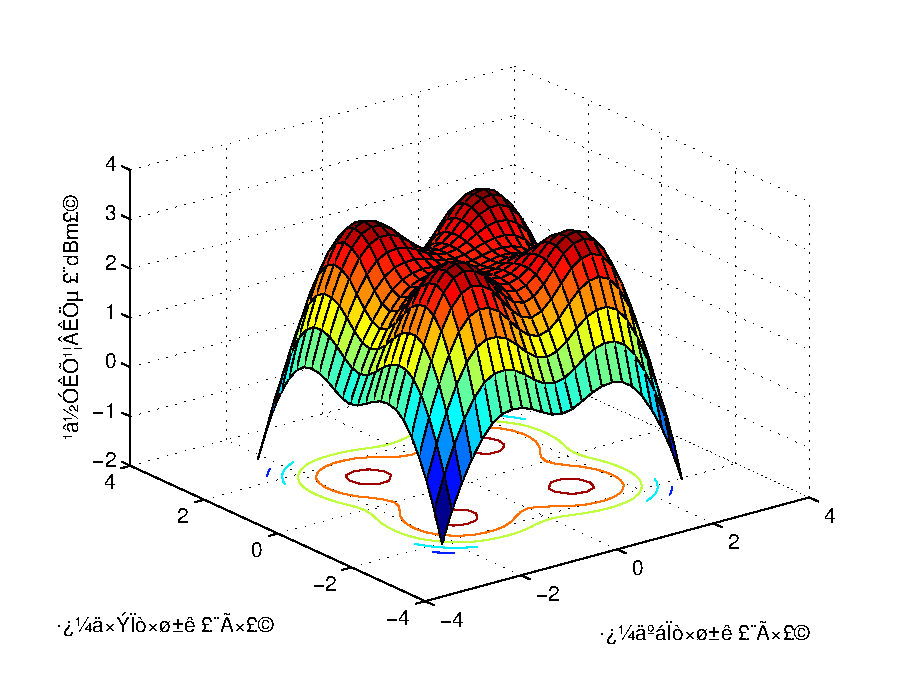
\includegraphics[width=0.7\textwidth]{figures/chapter-3/BestPower.eps}
	\caption{综合考量时的光接收功率分布}
	\label{fig:best_power}
\end{figure}

\begin{figure}[htbp]
    \centering
	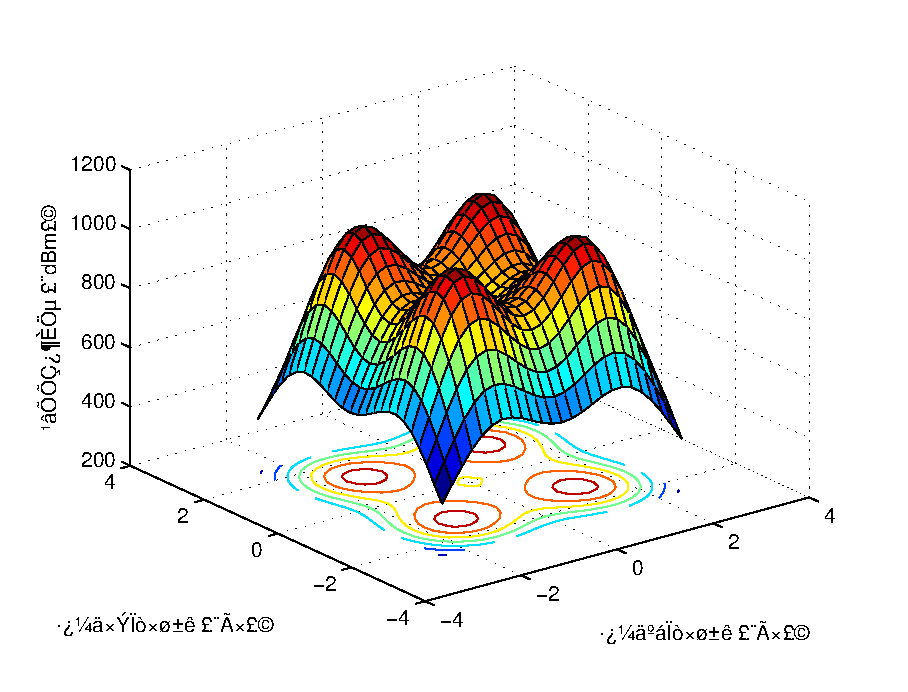
\includegraphics[width=0.7\textwidth]{figures/chapter-3/BestIllu.eps}
	\caption{综合考量时的光照强度分布}
	\label{fig:best_illu}
\end{figure}

从上图中,我们可以看到当系统要求兼顾指标的均匀度和光接收功率时,灯组的布局则可以看作为上述两种情况下的折中安置,不管是灯组距离室内中心点的距离还是灯组之间的间距,都处于一个比较平衡的值。
在该情况下得到的室内系统参数值为:光功率最大值为3.1840dBm,最小值为-1.7493dBm,平均值为1.7850dBm。光照强度最大值为1047lm,最小值为377lm,平均值为792lm。

在上述灯组布局下,可以看到灯组的分散放置使得室内光照和光通信的覆盖范围都得到了扩大,用户在除了墙角区域的其他区域都可以获得相对均匀地覆盖,
这样布局方式可以最大限度地扩大用户可进行可靠光通信的活动范围,也不易察觉到由于用户位置移动导致的通信质量的强烈变化。

在上述条件下的灯组布局,则是比较实用的灯组布局方式。可以看到这种布局方式,不仅可以保证室内的光照范围和光通信覆盖范围尽可能地广,
又可以保证在室内的大部分区域中的光接收功率较大,用户的高速通信需求可以得到保证。因此,这种综合考量下的布局方式可以在实际灯组的布局中获得应用。

\subsection{用户的接收视场角对最佳灯组布局结果的影响}
灯组的最优化布局结果不仅和当前的用户照明需求有关,还和用户的接收视场角有关系,这里可以研究用户的接收视场角对最佳灯组布局的影响。在仿真中,将模型公平性参数$\alpha$ 值设定为0.5,改变用户的接收视场角FOV的大小分别为40度和80度时,仿真得到的两种情况下最优化布局的光接收功率分布分别为

\begin{figure}[htbp]
    \centering
	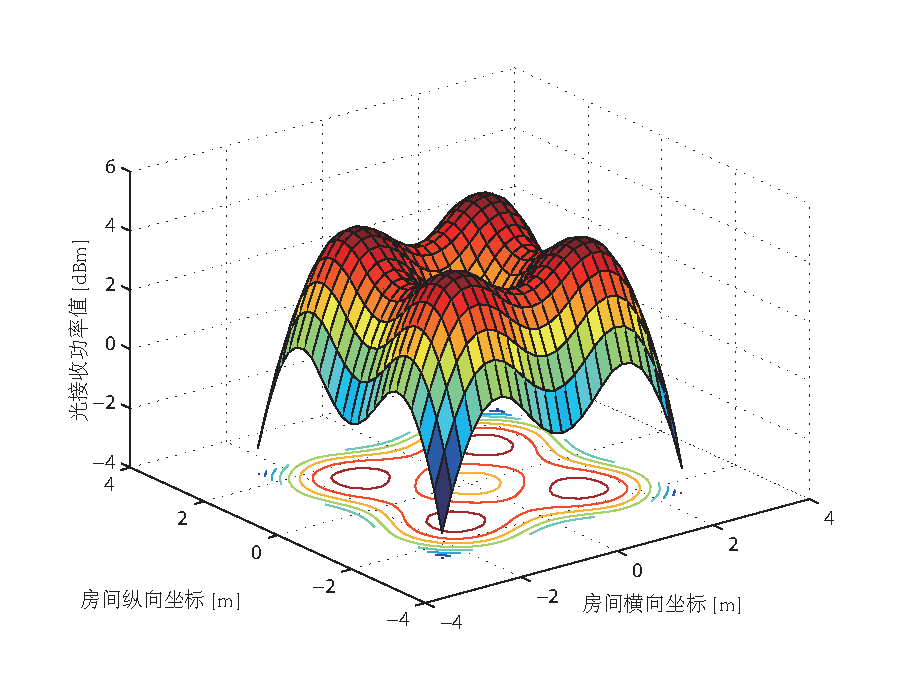
\includegraphics[width=0.7\textwidth]{figures/chapter-3/Fov40Power.eps}
	\caption{FOV值为40时的光接收功率分布}
	\label{fig:fov_40_power}
\end{figure}

\begin{figure}[htbp]
    \centering
	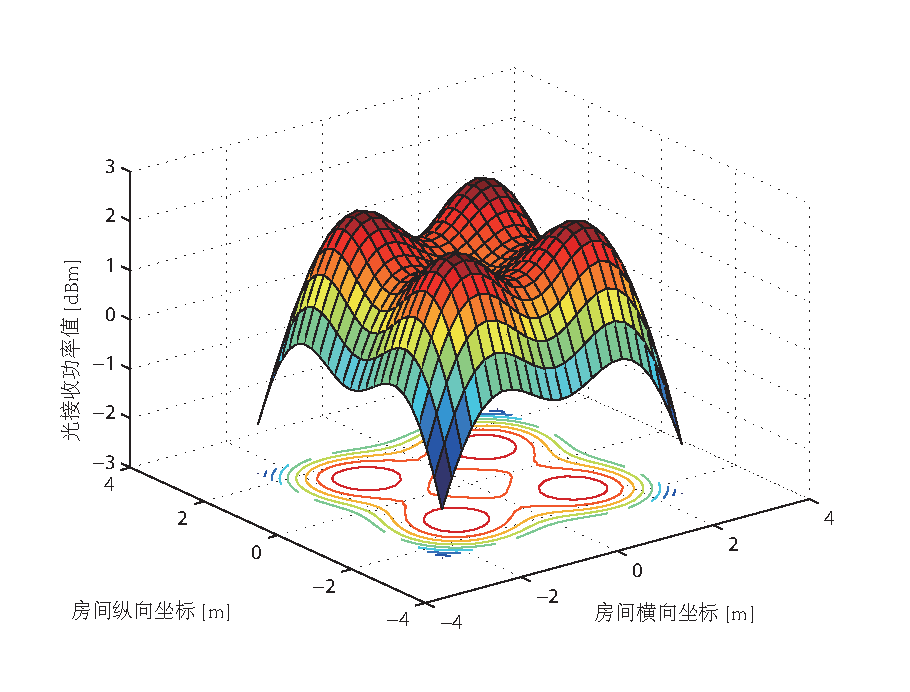
\includegraphics[width=0.7\textwidth]{figures/chapter-3/Fov80Power.eps}
	\caption{FOV值为80时的光接收功率分布}
	\label{fig:fov_80_power}
\end{figure}

上述直观地反映了FOV对光接收功率的影响,同时结合之前在FOV为60时仿真的数据,也可以通过下表中具体的数据来分析FOV的变化对灯组布局的影响。

\begin{table}[htbp]
    \caption{FOV的变化对灯组布局的影响}
    \label{tab:fov-vs-led-layout}
    \centering
    \begin{tabular}{lllllll}
        \toprule
        FOV值 & 最优d值 & 最优i值 & 光功率范围 & 平均光功率 & 光强范围 & 平均光强\\
        \midrule
        40度  & 1.3米  & 0.03米  & -3.1475 $\sim$ 4.4448dBm & 2.3580dBm & 350 $\sim$ 1017 & 800 \\
        60度  & 1.4米  & 0.02米  & -1.7493 $\sim$ 3.1840dBm & 1.7850dBm & 377 $\sim$ 1047 & 792 \\
        80度  & 1.4米  & 0.02米  & -2.0133 $\sim$ 2.4172dBm & 1.1109dBm & 377 $\sim$ 1047 & 792 \\
        \bottomrule
    \end{tabular}
\end{table}

从上表中可以看出,随着FOV角度的不断增加,其最优布局的平均光接收功率逐渐减小,而光接收功率范围的波动也在变小,表现在最终的灯组布局结果上,则是灯组距离房间中间的距离逐渐变大,
灯组之间的间隔也在随着FOV的增加而变小。而对于光照强度,在三种接收角度下,模型均能保证室内的光照强度处于一个较好的范围内,其均值都在800lm附近。这是因为当FOV的角度较小时,
用户只有在很小的范围内才能接收到灯组的信号,因此如果灯组之间的距离过远,那么在用户平面上的某些点时,用户收到的信号则会很微弱,某些点,如灯组的正下方,用户收到的信号又会很强,
所以灯组都被较为集中地放置,从而使得在FOV较小时牺牲了整体的均匀性,使得光接收功率上达到较优的状态。而随着FOV的逐渐增大,用户可接收到的灯组的范围也逐渐增加,这也就降低了之前让灯组集中布置的需求,
让灯组尽可能地分散开来布置,从而增加整体的均匀性,但是太多分散的灯组会降低整体的平均光接收功率,所以灯组之间的间隔就被逐渐地减小已作补偿,在均匀性和高光接收功率之间寻找一个平衡点。


\section{本章小结}
本章主要研究了室内可见光通信中灯组的最优化布局方式。首先,本章介绍了LED技术的发展历程和LED的发光原理,并介绍了室内照明中常见的度量单位。
接着,本章介绍了本文使用的室内光通信场景模型,并介绍了本文使用的LED灯的具体参数。对于如上提出的场景,本文根据室内照明和高速数据通信的需求,
提出了一种多目标的灯组布局最优化模型,充分考虑了室内照明和接收功率均匀度和光接收功率均值的影响。在模型的解决阶段,本章使用了线性加权法对模型进行了求解,
并通过调节模型中的参数因子,分别求解出对于高室内光照和光接收功率均匀度,高平均光接收功率,和综合考虑上述两种条件这三种情形下的灯组的最优分布,并分别给出了其相应的光接收功率分布和光照强度分布。

    % !Mode:: "TeX:UTF-8"
% 调制技术与其它基带技术的研究

\chapter{分布式组网光通信系统的灯组调度}\label{chap:baseband-technology}
\section{引言}
对于一个安装有多个灯组的房间来说,为了保证用户和灯组之间的高效无缝的通信,需要设计一种灯组调度算法,来实现多用户的通信,并适应移动用户的移动性需求。
通常对于灯组的种类划分,可以分为两种,一种是实现均匀照明覆盖的灯组,这种灯组通过使用多个宽角度的LED芯片,使得每个LED灯组的覆盖范围较大。而另外一种是射灯照明的灯组,
这种灯组的方向性较为明显,其灯组的覆盖方位也较小[49]。在本章中,我们先研究第一种灯组室内组网的情况。本章将首先介绍分布式组网光通信系统的基本结构,
在给出本章提出的一种灯组调度算法,来解决该架构下移动用户的灯组调度问题。

\section{分布式组网光通信系统分析}
对于多个大覆盖范围的LED灯组的组成的室内光通信系统,为了保障对移动用户的支持,又避免实现复杂的灯组切换机制,本章采用了分布式的灯组组网布局。
这里的分布式是指所有的灯组的数据传输到受到调度器的控制,当调度器允许当前灯组和某用户进行通信时,所有的灯组将会发送相同的信息与该用户进行通信。
以一个房间内含有四个灯组为例,其分布式灯组网络架构如下图所示。

\begin{figure}[htbp]
    \centering
	\includegraphics[width=0.8\textwidth]{figures/chapter-4/DistributionOverView.eps}
	\caption{布式灯组网络架构}
	\label{fig:distribution-overview}
\end{figure}

图中,四个灯组和调度器相连,下图的圆圈表示的是灯组的覆盖面积,图中用户1处于灯组3的覆盖区域,用户2处于灯组3和灯组4的共同覆盖区域中。

\subsection{本文采用的上下行信道}
由于光通信系统上下行数据传输的不对称性,同时为了避免上行链路电路的复杂度,在本系统中下行使用光通信信道,上行使用红外信道进行数据传输。
红外通信作为一种最常见的室内短距离无线通信技术,早就在短距离通信中得到广泛地应用,其技术也已经较为成熟。本系统将光通信和红外通信相结合,既可以简化系统的复杂度,又可以保障系统的性能。其通信结构如下图所示。

\begin{figure}[htbp]
    \centering
	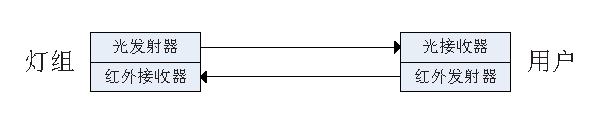
\includegraphics[width=0.8\textwidth]{figures/chapter-4/DistributionChannel.eps}
	\caption{分布式组网光通信系统采用的上下行信道}
	\label{fig:distribution-channel}
\end{figure}

在灯组侧,拥有光发射器和红外接收器,而在用户侧拥有光接收器和红外发射器,当灯组有数据需要发送给用户时,就使用光发射器将数据经过光信道发送出去,
而用户发送数据时,则使用红外发射器将数据发送出去。这样,由于上下行采用的是不同的信道,因此上下行通信互不影响,类似于采用频分复用进行上下行通信的系统。
在本系统中,由于所有的灯组都安装了红外接收器,并且一直处于打开的状态,因此,当用户通过红外发射器发送数据后,其周围的灯组都是可以接收并获得该用户的数据。

\subsection{多用户通信方式}
对于多个移动用户的场景,本系统采用的方式为基础的时分复用技术,即将用户安排在不同的时隙上进行用户的服务。
这种方式对室内的移动用户的数目有一定的要求,但是在常见的室内光通信系统中,尤其是常见的办公室和会议室,使用的用户数目一般都不会很多,因此,采用时分复用进行多用户通信是简单而又合理的。

由于在分布式组网条件下,灯组的作用相当于一根发送天线,用户的移动将不再受到灯组位置的制约,但是用户的移动将会影响到发送灯组集合的选择,所以,下面将讨论对于移动用户的灯组调度策略。

\subsection{分布式组网调度策略分析}
在实际的通信过程中,如果对于每一个用户而言,每次的通信可以直接使用房间内所有的灯组共同和用户进行数据传输,无疑是最为简单的方式,也不需要考虑用户在灯组的切换,但是这种方式会导致某些灯组发送的信息根本就不会被用户接收到,
从而造成大量的资源浪费。因此,需要一种合适的灯组调度算法,在分布式灯组组网的架构下,根据用户的移动中的需求分配相匹配的灯组资源。

传统的调度方法是使用下行信道广播灯组的信息,当用户接收到多个灯组的信息后,再通过上行传输,反馈接收到的灯组信息和信号强度信息给调度器,调度器通过此信息选择合适的灯组集,这种调度方式使得灯组的配置过程需要在上下行两个过程之后才能完成,影响数据的正常传输,耗费系统开销,
同时灯组集选择是依据当前的灯组接收信号强度来进行的,没有考虑到用户的移动情况。其中有一种调度方法是以灯组接收信号强度最大化为准则进行灯组的选取,这种方式能快速选择可使用灯组,却不能使用户得到多个灯组的协作,另一种方式是以灯组接收信号强度判决可服务的灯组作为灯组集服务用户,
这种方式引入了灯组间的协作,但是判决的依据只是当前的接收信号强度,从而得到的灯组调度结果有一定的局限性。在分布式灯组组网的条件下,可以通过合理地选择更加准确的灯组集合联合发送用户数据信息来解决这个问题,通过相邻灯组的协同工作,来保障用户在移动中的通信质量。

\section{基于运动方向的灯组协同调度}
\subsection{判决变量依据}
不同于上述提及的其他系统中使用上下行传递和反馈信息的方式来进行灯组的选择,本系统中测量的是数据传输中用户给灯组发送应答数据时的灯组接收功率。根据上述的信道介绍,上行采用的是红外信道,于是当用户采用红外信道上行发送灯组传输数据的应答信息时,
上方的多个灯组都有可能接收到用户的应答信息,此时灯组接收到的信号强度则可作为系统的灯组调度的输入参数。

使用上述方式,可以直接利用数据传输中的信息进行灯组的调度,从而可以避免造成额外的系统开销和操作复杂度。但是由于上下行的信道不对称性,收到用户应答信息的灯组并非就是可以给用户发送数据的灯组,所以当灯组接收到用户应答信息后,
仍然需要判别用户是否处于该灯组的覆盖范围内。判决的门限值为设定当用户处于光通信覆盖区边缘时在反向信道灯组接收到的接收信号强度,设该值为$P_{th}$。同时由于灯组接收到用户的信号强度是动态变化的,所以不能直接根据接收信号值大于$P_{th}$就认为可以使用该灯组为用户提供服务,
而应该使用迟滞判决方案,假设灯组$A_{i}$接收到用户数据的接收信号强度为$P_{i}$,则当其满足以下公式时,可以认为用户处于灯组$A_{i}$的覆盖范围内。

\begin{equation}
    P_{i}-P_{th} > P_{hy}
    \label{equ:user-enter-hy}
\end{equation}

其中,$P_{hy}$即为判决的迟滞门限值。

\subsection{用户的运动方向判别}
如果系统只知道灯组的接收信号强度信息,根据式()可以判决出当前可以为该用户服务的灯组集,从而使用这个灯组集为用户提供数据传输服务。
这种方式其实也就等效于上述提及的通过下行广播,再将接收到的广播的数据上行告诉调度器进行灯组调度的方式。但是这种方式会产生一定的问题,
如当用户的移动速率过快时,或者是调度的周期过长时,用户容易走到调度灯组集合的边缘区,甚至是离开当前灯组集的覆盖范围。比如说,当一个用户处于一个灯组的核心区时,
此时进行了灯组的调度,将为该用户的灯组确定只使用当前灯组,但是考虑到随着用户的移动,在下一个调度时刻来临时,有可能该用户已经移动到了该灯组的边缘或者移动出该灯组的覆盖范围了,
导致在该段调度时间内,该用户并没有被很好地服务到。

该现象发生的主要原因就是当系统进行灯组调度时,依据的是当前的灯组接收信号强度信息,因此得到的调度结果仅仅对当前时刻是最优的,并不能保证在整个调度时间的最优。
要想得到调度周期内的最优灯组调度,还需要知道用户的运动的趋势,这才可以使我们了解到将来可以覆盖到该用户的灯组,从而可以更好地为用户提供服务。
而对于该用户的运动方向信息的获取,我们可以从多次的灯组的接收信号强度中分析得到,因为灯组接收信号强度的变化可以反应一定的用户移动方向信息。

由于系统的反向链路使用的是红外信道,依据其传输模型[50],红外通信在自由空间中的$LOS$的路径损耗主要和用户和灯组之间的距离$d$和光传播到用户接收平面的入射角度和用户的接收视场角有关。
而当用户向上发送红外数据时,在用户附近的灯组在接收光功率的路径损耗,可以近似正比于用户和灯组之间距离的平方[51],接收电功率的路径损耗则可以近似正比于用户和灯组之间的距离的四次方,
因此类似于距离-路径损耗模型,可以通过下式根据参考值计算出某一灯组测量到的功率所对应该灯组和用户之间的距离值

\begin{equation}
    \frac{{{P_0}}}{{{P_i}}} = \frac{{\frac{1}{{d_0^4}}}}{{\frac{1}{{d_i^4}}}}
\end{equation}

其中$P_{0}$和$d_{0}$分别为灯组和用户之间的参考距离和参考功率,$P$和$d$为灯组测量到的电接收功率和所需要计算的灯组和用户之间的距离。假设灯组距离接收平面的高度$h$是已知的,那么此时可以获得用户距离某灯组$A_{i}$之间的水平距离

\begin{equation}
    {x_i} = \sqrt {d_i^2 - {h^2}}
\end{equation}

这样,利用某一个灯组在本次调度和上一次调度时刻分别接收到的信号强度$P_{ni}$和$P_{bi}$,就可以对应地求出本次调度和上一次调度时刻用户距离该灯组的水平距离$x_{ni}$和$x_{bi}$,进行可以使用该水平距离的差值 来描述该用户对于灯组$A_{i}$的运动趋势

\begin{equation}
    \Delta {x_i} = {x_{ni}} - {x_{bi}}
\end{equation}

当该值为正时,说明该用户正在远离灯组$A_{i}$,否则说明该用户正在靠近灯组$A_{i}$。
通过上述的分析,系统就可以在调度时刻,不仅能获得当前的用户反向接收信号强度信息,并且可以获得用户相当于各灯组的运动方向信息。

但是如果所有灯组信号强度$P_{ni}$和$P_{bi}$都相差较小时,这就说明当前用户在所在位置中运动的幅度较小,不足以进行判断。
在这种情况下,系统将会直接使用上次的调度结果为该用户提供服务。所以,需要设置一个用户运动检测门限,
按照式()中的判别依据,当所有的灯组的接收信号强度变化都小于该门限$\Delta P$,那么调度时就认为该用户在调度期间内没有进行运动。

\begin{equation}
    \left| {{P_{ni}} - {P_{bi}}} \right| \le \Delta P
\end{equation}

\subsection{基于用户运动方向的信号强度补偿}
当系统在调度时刻,获得到用户的运动方向信息之后,则可以将其运用到灯组调度的决策中来。
为了能在用户移动的过程中更好地服务用户,在灯组的调度时,需要考虑的不仅是当前可以为用户提供服务的灯组,
还需要考虑在调度期间可能会给用户提供服务的灯组。所
以,系统可以利用上述获得用户的运动方向信息对灯组获得的接收信号强度信息进行了修正,从而获得更好地灯组调度结果。

由于短时间用户的运动趋势不太可能发生改变,因此当前用户运动方向上的灯组就有可能是将来可以为用户提供服务的灯组,
对于这些灯组而言,系统需要给予它们一定的鼓励,以增大这些灯组在依据式()中的判决准则下会被选中的可能性。
所以,首先可以根据运行方向的信息,将所有的灯组分为两个集合,即用户前进方向灯组集和远离方向灯组集。
对于前进方向的灯组集中的灯组获得的接收信号强度信息进行功率补偿以适应用户移动的需求。

因为如果用户移动的方向更接近于某灯组,那么该灯组就更有可能会在之后为用户提供服务强度,
可以定义用户趋向于某灯组的程度称为趋向度。补偿遵循的原则是用户对某灯组的趋向度越好,该灯组的强度补偿就越高。
这里用户对于某灯组的趋向度采用用户在当前调度时刻和上一调度时刻上的水平距离的距离差表示。
对于所有灯组中用户趋向度最高的灯组,给予最大的强度补偿$\delta_{\max}$,其他的前进方向上的灯组也与对该灯组的趋向度有关,按照下式进行。

\begin{equation}
    {\delta _i} = \frac{{\Delta {x_i}}}{{\max \Delta {x_i}}}*{\delta _{\max }}
\end{equation}

其中,$\delta _i$记为对于灯组$A_{i}$的接收信号强度补偿。

通过上述的补偿算法,可以更好地将用户相对于灯组的运动方向信息转变为对灯组接收信号强度的修正,从而获得更好的灯组调度效果。

\subsection{基于运动方向的灯组协同调度}
根据上述分析,可以总结出本文提出的基于用户运动方向的灯组协同调度算法,其算法的主要思路为首先利用获取的灯组反向信道接收信号强度值,
计算出终端用户相对于各灯组的位移,并利用该位移信息将所有灯组分为靠近灯组集和远离灯组集。
在对靠近灯组集中的灯组进行接收信号强度修正后,再根据所有灯组接收信号强度值决定灯组配置方案。
该灯组调度算法充分地考虑到分布式组网架构下系统的特点,可以在室内光通信通信时为用户提供最佳的通信灯组集合,
从而保证在整个用户平面上,甚至是灯组的边缘区,灯组和用户通信的可靠性。

该算法的流程图如下图所示:

\begin{figure}[htbp]
    \centering
	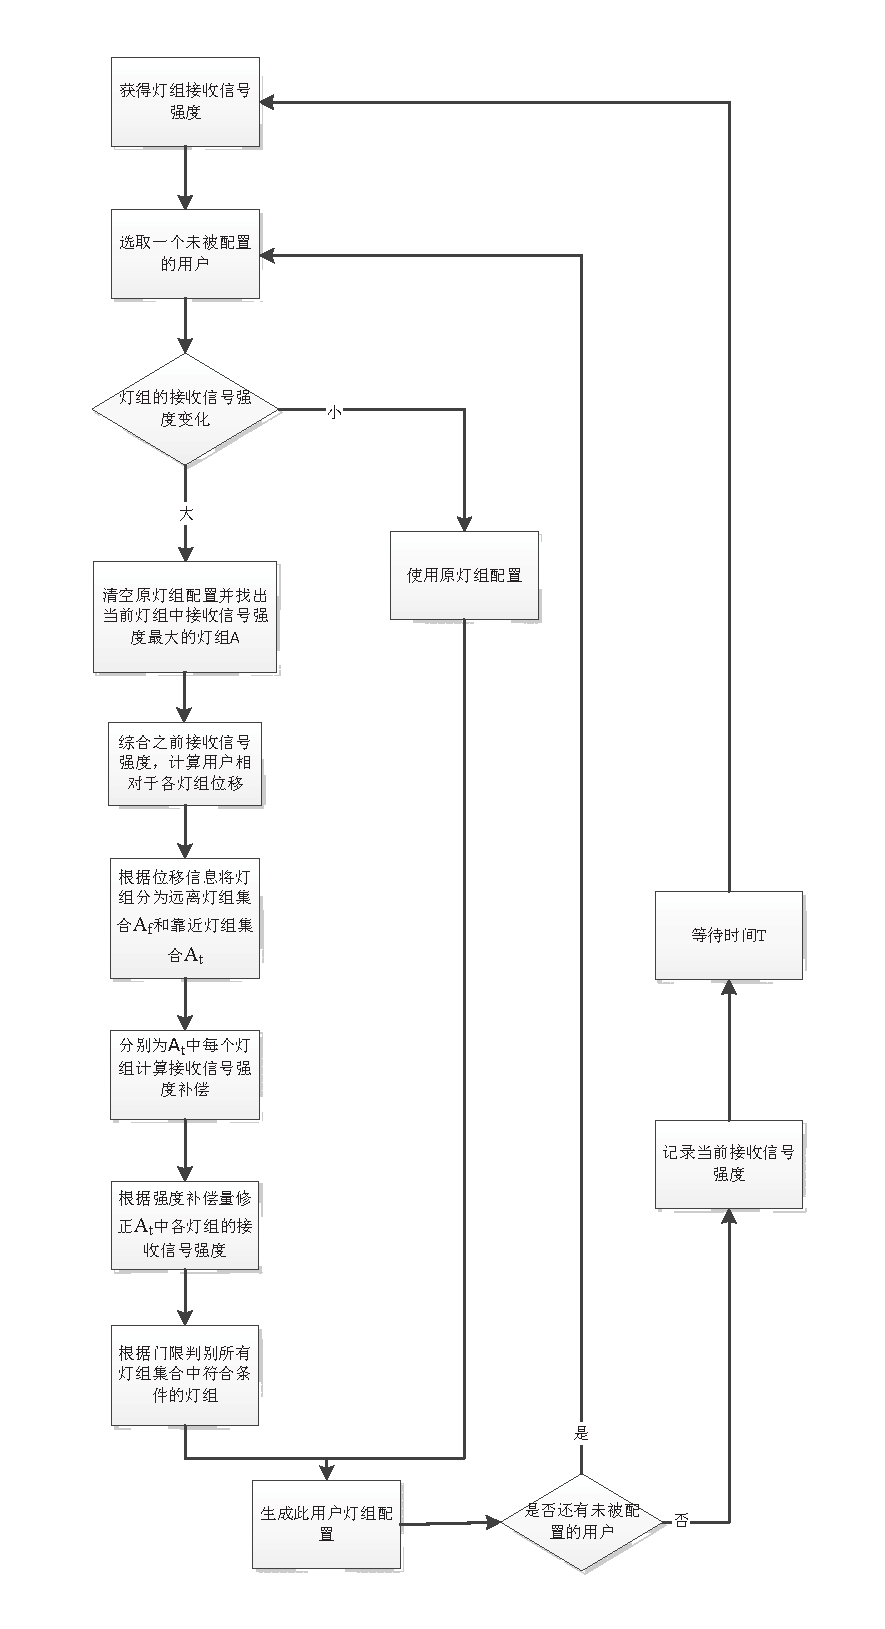
\includegraphics[width=0.8\textwidth]{figures/chapter-4/DistributionSchemeFlow.eps}
	\caption{基于用户运动方向的灯组协同调度算法流程图}
	\label{fig:distribution-scheme-flow}
\end{figure}

如上图所示,算法中的主要过程可以描述如下:

第一步,调度器获得各灯组的反向信道接收信号强度信息;
第二步,选取一个未进行灯组配置的用户,如果每个灯组的接收信号强度变化都在门限值$\Delta P$之内,则直接使用原灯组配置,并进入第八步,如果存在一个灯组的接收信号强度变化超过门限值$\Delta P$则清空原灯组配置信息;
第三步,调度器根据当前的接收信号强度测量结果和前一次灯组配置时的接收信号强度测量结果,通过式()计算出用户在这段判决周期中相对于灯组$A_{i}$移动的位移$\Delta x_{i}$:
第四步,在所有灯组中,将位移$\Delta x_{i}$为正的灯组归为靠近灯组集合$A_{t}$,将位移$\Delta x_{i}$为负的灯组归为远离灯组集合$A_{f}$;
第五步,对于靠近灯组集合$A_{t}$集合中的灯组,利用方向信息$\Delta x_{i}$按如下公式计算出强度修正值 ;
第六步,对靠近灯组集合$A_{t}$中第$i$个灯组的接收信号强度$P_{i}$按照下式进行修正,得到修正后的接收信号强度值$\overline{P_{i}}$;
第七步,判断靠近灯组集合$A_{t}$集合中修正后的接收信号强度值$\overline{P_{i}}$是否满足\eqref{equ:user-enter-hy},若满足则将对应灯组i记入灯组配置结果集合中;同时,判断远离灯组集合 中没有经过修正的灯组接收信号强度是否满足\eqref{equ:user-enter-hy},将满足条件的灯组记入灯组配置结果集合中;
第八步,生成此用户的灯组配置集合,判断当前是否还有未配置的用户,若有未配置的用户,返回第二步,否则,当前获得的修正前的灯组接收信号强度数据放入数据库中;
第九步,调度器等待一个调度时间周期$T$,返回第一步进入下一次灯组调度流程。

\section{仿真实验及结果分析}
为了验证本文所提出的基于用户运动方向的灯组协同调度算法的有效性,本文在NS2平台上搭建了室内可见光通信的平台,并通过修改了NS2底层的源代码进行算法的性能仿真。
为了与本文提出的方法进行对照,在实际的仿真中,也使用了另外两种调度算法进行对照实验。一种调度算法为非协作的最优灯组选择算法,即在灯组的选择过程中,总
是选取接收强度最大的那个灯组,也就意味着是距离用户最近的那个灯组。另外一种调度算法为可用灯组协作的灯组选择算法,即依据当前获得的灯组接收功率,选择那些可以为用户提供服务的灯组组成灯组集为用户提供服务。

仿真中的场景设置为在一个房间内安装有四个灯组,由于系统对单个用户和对多个用户的调度过程是相同的,因此,可以假设一个用户在场景中进行按照如下轨迹进行运动。

\begin{figure}[htbp]
    \centering
	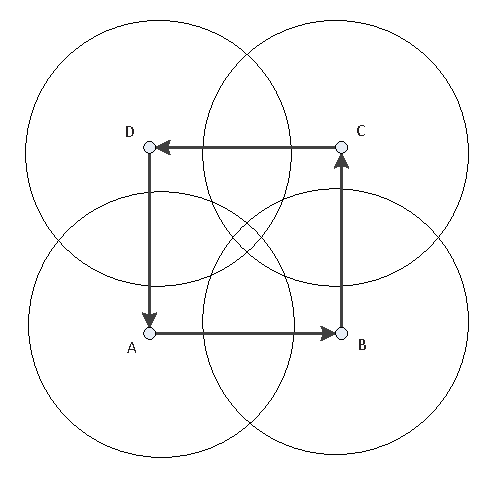
\includegraphics[width=0.8\textwidth]{figures/chapter-4/DistributionUserMove.eps}
	\caption{仿真中的用户运动轨迹图}
	\label{fig:distribution-user-move}
\end{figure}

在本文仿真中,假设用户沿着上述的位置进行移动,已验证算法对用户移动性的支持。灯组的调度算法主要目的就是使用最为合适的灯组为用户服务,从而避免使用全部的灯组进行数据传输,造成资源的消耗。
而当用户处于某灯组的正下方附近时,其光接收功率是比较强的,传输性能也较好,所以灯组的调度其实质就是解决用户处于灯组的边缘区时,多个灯组协同工作进行数据传输这个问题。
所以,为了验证调度性能的好坏,本文仿真中使用灯组的数据重传次数来定量地衡量系统的性能。灯组发生数据的重传就意味着当前的灯组和用户的数据通信存在问题,大量的数据重传发生则意味着用户的当前的通信质量较差。

\subsection{最大修正门限值对算法的影响}
由于算法中使用了接收信号强度补偿,其每个灯组的强度补偿量与最大强度补偿量有关,为了研究最大强度补偿量对算法性能的影响,本文在调度时间为0.6s,
用户的速度为1m/s的情况下,进行了仿真,其中最大修正门限值分别取迟滞门限的0-5倍。得到的结果如下:

\begin{figure}[htbp]
    \centering
	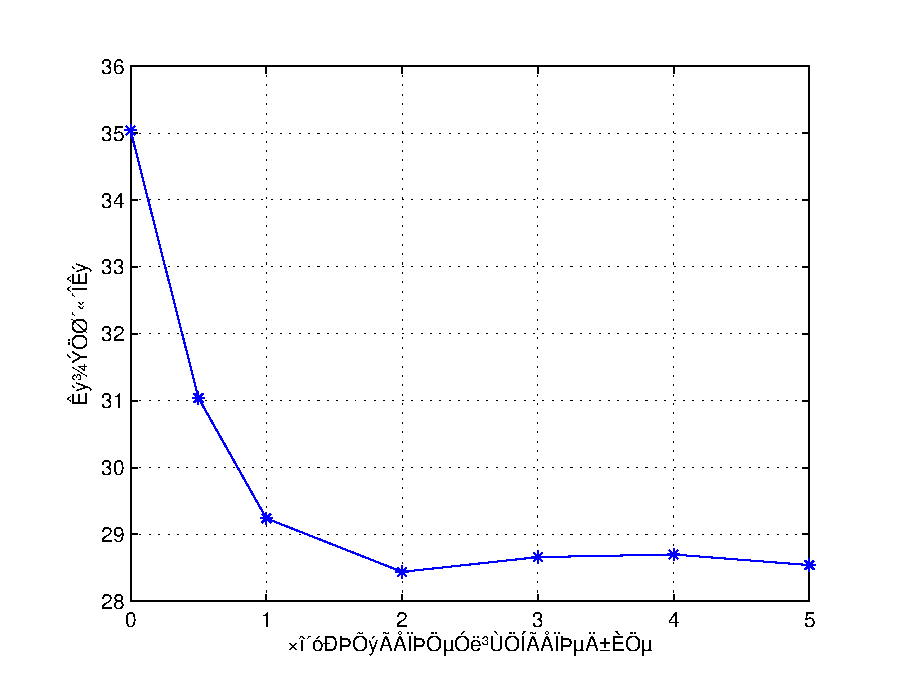
\includegraphics[width=0.8\textwidth]{figures/chapter-4/DistributionBiggestModify.eps}
	\caption{最大修正门限值对系统性能的影响}
	\label{fig:distribution-biggest-modify}
\end{figure}

从上图中可以发现,随着最大修正门限值的增大,数据重传次数先开始下降,在1.5倍之后开始趋于一个稳定值。
这是因为随着最大修正门限值的增大,用户前进方向的灯组的强度修正也就相应增大,这样可以使得在用户未到达某些灯组前,就将该灯组的数据传输通道打开,
当灯组一进入该灯组范围就可以接收服务,但是随着修正门限值的不断增大,虽然灯组的打开时间不断被提前,使得用户在距离该灯组的很远的位置灯组就被打开,
但是灯组在之后的时间内并不能服务到该用户,而需等到用户进入后才能进行系统传输,所以灯组的过早的协作并不能减少数据重传。在下文的仿真中,最大修正门限值取2倍于迟滞门限值。

\subsection{不同的灯组半功率角系数下各算法性能的比较}
在进行LED灯组组网中,灯组的种类选择对最终组网的质量有着重要的影响,而灯组的种类选择主要体现在灯组的半功率角系数这个参数上。灯组的半功率角系数是由灯组的半功率角定义的

\begin{equation}
    m =  - \frac{{\ln 2}}{{\ln (cos{\Phi _{1/2}})}}
\end{equation}

其中,$\Phi _{1/2}$就是灯组的半功率角,代表灯组在包含主瓣最大辐射法相的某一个平面内,相对最大辐射方向功率通量密度下降到一半处的方向和最大辐射方向的夹角。该值可以表征灯组的聚光程度,不同种类的LED灯其半功率角不同。

在本文的仿真中,在不同的半功率角系数下仿真了三种算法在数据重传次数方面的表现,其仿真结果如下所示

\begin{figure}[htbp]
    \centering
	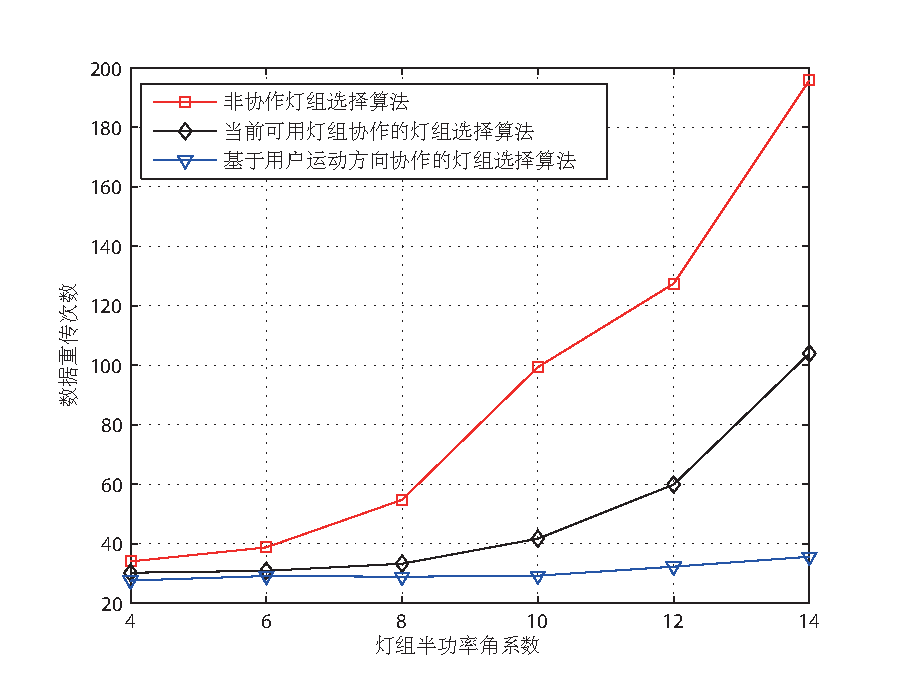
\includegraphics[width=0.8\textwidth]{figures/chapter-4/DistributionLedParam.eps}
	\caption{灯组半功率角系数对系统性能的影响}
	\label{fig:distribution-led-param}
\end{figure}

当m值较小时,也就意味着灯组的半功率角较大,此时灯组的功率辐射较为分散,在灯组的边缘区也有很好的接收功率强度,可以从图上看到,
此时的三种算法得到的数据重传次数都较少,也就意味着系统的性能都较好,因为在这种情况下,三种不同的算法不管有没有进行灯组协作,
都可以在重叠覆盖的边缘区获得较好的通信质量,而采用灯组协作的后两种算法性能会略优越于非协作的算法。随着m值的增加,灯组的半功率角逐渐减小,
也就意味着灯组的功率辐射变得更加集中,因此,此时在灯组的边缘区用户的光接收功率将大大降低。所以从上图中可以看到,这种情况下,若使用非协作算法,
用户在灯组边缘区的通信质量将会非常差,在使用可用灯组进行协作之后,数据重传量将会大幅降低,但是由于其调度的局限性,其协作性能仍然较差。
而在使用本文基于方向的灯组协同调度算法后,显著提高了灯组的协同调度效果,使得系统的通信质量得到进一步的提升。

\subsection{不同的接收视场角下各算法性能的比较}
同样对系统的仿真系统存在影响的还有用户的接收视场角视角(field of view, FOV),用户的接收视场角将会影响灯组的覆盖范围,从而改变用户移动时对灯组的调度。本文在调度时间为0.6s,用户的速度为1m/s的情况下,分别对FOV从30度到60度进行了仿真,以研究其对于算法性能的影响。

\begin{figure}[htbp]
    \centering
	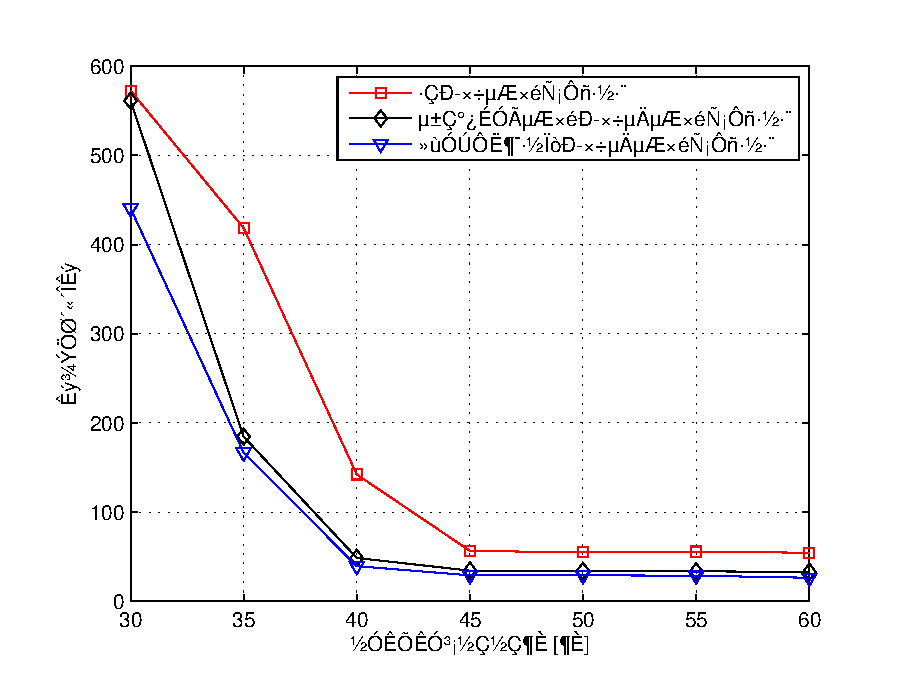
\includegraphics[width=0.8\textwidth]{figures/chapter-4/DistributionUserFov.eps}
	\caption{接收视场角对系统性能的影响}
	\label{fig:distribution-user-fov}
\end{figure}

上图展示了三种不同的灯组调度算法在不同的FOV的情况下的性能变化。可以看到,随着FOV的增大,三种算法的数据重传都出现大幅地减少,这是由于当灯组的FOV较小时,灯组的重叠区覆盖就很小,
用户在灯组的边缘不太容易获得灯组的协作,就算在用户在边缘区得到灯组的协作,其协作效果也并不理想。但是当FOV增加后,本文的灯组协同调度算法将可以充分利用灯组的共同覆盖,
进行灯组间的协同进行数据传输。但如果FOV持续的增大,系统的性能指标却趋于稳定了。这是因为随着FOV的不断增大,虽然灯组的重叠区变大了,但是由于用户在灯组的正下方附近的灯组核心区本身传输质量就很好,
并不需要其他灯组的协作就能保证很好的数据传输,所以较大的FOV也并不能继续提高系统的性能,另一方面,在室内可见光通信中,广角的LED灯组的研究本身就受到器件水平等方面的限制,不太容易被实现,
所以使用合适的FOV角度对室内光通信的灯组调度具有重要的意义。而对于非协作算法而言,当FOV较小时,运动中的用户易于移动到某个灯组的边缘区,甚至是移动出某一灯组的覆盖区域,
因此,这将导致非协作调度方式在FOV较小的情况的数据重传量将非常大。但FOV逐渐增大之后,用户在边缘区运动时才能在信号质量不佳时,接收到其相邻的信号质量较好的灯组的信号,保证通信质量。
对于当前可用灯组协作的灯组选择算法而言,FOV的增大则可以增加用户在边缘区可以使用的协作灯组数,因此,当FOV增加后其数据重传会大幅下降,但是同样由于其调度的瞬时性,因此其性能没有本文提出的算法优越。

\subsection{不同的系统调度时间下各算法性能的比较}
另外,为了验证本文提出的算法性能,我们在不同的系统调度间隔下比较了本文提出的算法和上述提到的两种算法之间的性能。其结果如下所示

\begin{figure}[htbp]
    \centering
	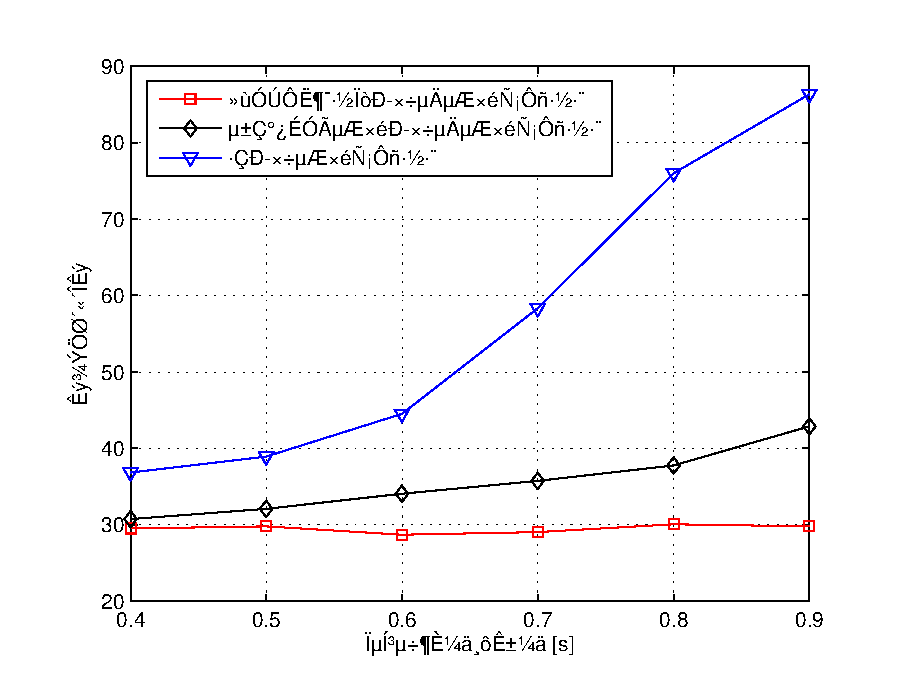
\includegraphics[width=0.8\textwidth]{figures/chapter-4/DistributionSchTime.eps}
	\caption{系统调度时间对系统性能的影响}
	\label{fig:distribution-sch-time}
\end{figure}

从上图中,可以看到,随着系统调度间隔时间的增大,非协作的灯组选择方法的性能将会越来越差,而当前灯组协作的灯组选择方法虽然随着间隔时间增加性能也越来越差,但是其性能优于非协作灯组选择算法。
而本文提出的基于运动方向协作的灯组选择方法随着调度时间的变化波动较小,且性能优于上述两种方法。这是因为系统调度间隔的增大,将会使得调度的周期增加,如果使用非协作灯组选择方法,
用户在边缘区的接收信号质量将会很差,导致大量的重传发生。在使用当前灯组协作的灯组选择方法后,当用户处于边缘区时,若调度及时,多个灯组会协同工作进行下行数据传输,但是如果调度时间过长,
也有可能导致用户不能及时地获得多灯组的协作。而本文提出的基于用户运动方向协作的灯组选择方法,则可以克服上述的弊端,当调度周期很长时,利用对用户的运动方向预测,提前进行灯组的协作,从而提高系统的协作性能。

\subsection{不同的用户移动速度下各算法性能的比较}
在将系统的调度周期设定为0.6s之后,本文又对不同用户运动速度下,系统采用不同的调度方法的情况进行了仿真研究,其结果如下图所示

\begin{figure}[htbp]
    \centering
	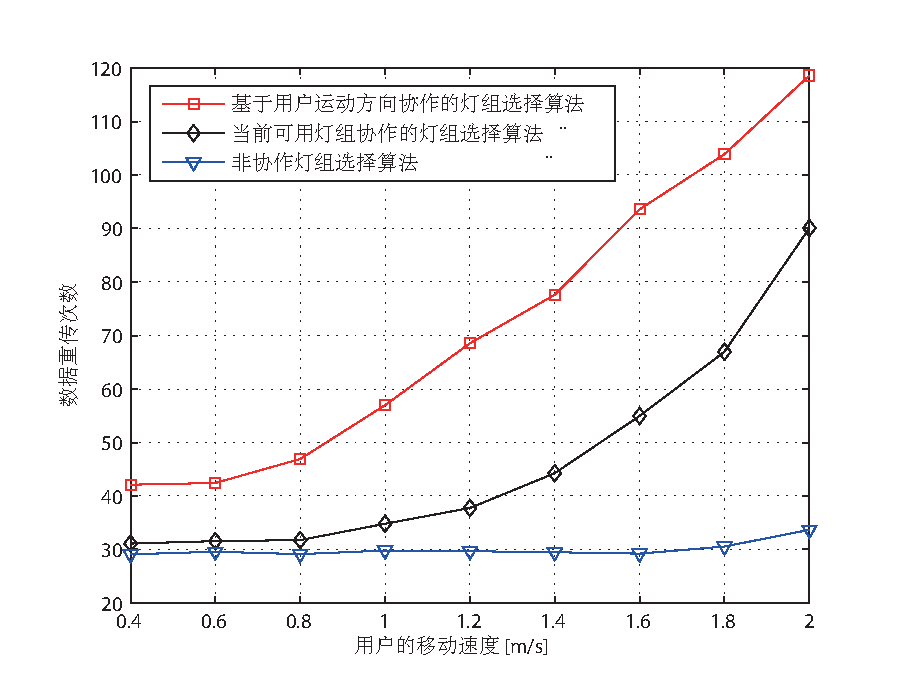
\includegraphics[width=0.8\textwidth]{figures/chapter-4/DistributionUserSpeed.eps}
	\caption{用户移动速度对系统性能的影响}
	\label{fig:distribution-user-speed}
\end{figure}

对于上图,从横向看,可以发现随着用户的移动速度的不断增加,使用三种灯组选择方法的性能都会出现一定程度的恶化。但是非协作灯组选择和当前可用灯组协作这两种方法的系统性能下降较为严重,而对本文提出的基于运动方向协作的方法的性能影响较小。
从纵向对比,可以看到,本文提出的方法的性能要优于另外两种灯组选择方法。在用户的速度达到2m/s时,数据重传次数只有非协作灯组选择方法的约25\%,是当前可用灯组选择方法的30\%。
这是因为随着用户速度的增加,若采用非协作灯组选择方法,用户在调度周期中将会更有可能移动出原先调度灯组的覆盖范围,且由于非协作灯组选择只使用一个灯组服务用户,边缘区的信号质量会很差,所以非协作灯组选择方法的系统性能是最差的。
而当我们采用了当前可用灯组协作的灯组选择方法后,虽然用户在边缘区会受到多个灯组的协同工作进行数据传输,但是较快的用户移动仍然可能会引起用户移动出原先调度的灯组集,使得系统系能指标得不到保障。
但在使用了本文提出的灯组选择方法后,由于在灯组的调度时,由于增加了用户的位置信息,可以在灯组的调度中包含了将来可以使用中的灯组,从而避免由于用户的移动造成的用户在调度周期内在边缘区重传次数过高的问题。

\section{本章小结}	
本章主要研究了在分布式灯组布局下的灯组协同调度问题。这里的分布式灯组布局是指,所有的灯组只负责物理层的数据传输工作,而不涉及具体的用户控制等功能,而数据的传输控制由连接各灯组的调度器负责。
本章首先介绍了分布式灯组布局的概念,并介绍了本章所提及系统的上下行信道,多用户通信方式等内容,在此基础上,本章利用用户进行数据传输时的功率测量,提出了一种基于用户方向的灯组协同调度算法,在进行灯组的调度时,
不仅考虑测量到的用户的上行功率,并考虑到用户的移动方向,从而获得更加准确的调度灯组,当用户移动到灯组的边缘区时通过调度好的灯组协同进行下行数据传输。最后,本章在NS2平台上进行了算法的仿真,并和另外两种灯组调度算法进行了对比,
仿真结果表明,本文提出的算法在灯组边缘区可以获得更好的灯组协作效果,对比其他两种调度算法有着较大的优势。

    % !Mode:: "TeX:UTF-8"
% 独立式组网光通信系统的灯组调度

\chapter{独立式组网光通信系统的灯组调度}\label{chap:independent-led-design}
\section{引言}
在上述的分布式组网的架构中,所有的灯组都被调度器控制,从而增大了灯组在房间内的覆盖范围,通过合理的调度方式可以提高了灯组的通信质量,但是这种组网方式没有采用多用户的空分复用技术,系统容量不够高。
本章要研究的系统架构则是独立式的灯组架构,即每个灯组可以独立地控制用户的接入,信息的传输,类似于无线局域网的接入点的概念。基于这种独立式的灯组架构,在多用户的情况下可以采用合理的调度策略,
在保证用户之间没有干扰的前提下,尽可能地提高系统的容量。同时,还需要考虑到用户移动的情形,灯组的调度必须能够适应用户的移动,保证在大量用户运动的条件下,仍然可以获得有效的调度结果。

\section{独立式组网光通信系统分析}\label{sec:analysis}
\subsection{独立式组网光通信系统的调度要求}
为了进行合理的独立式组网灯组调度,首先,需要了解该灯组架构下光通信系统中多用户通信下的调度要求,本文总结了以下四点:

\begin{enumerate}
    \item 在可见光通信系统中,为了满足光照覆盖的要求,通常需要在室内安装多个灯组进行照明,由于每个灯组的覆盖范围有限,
        安装的多个LED灯组一般在室内广泛分布,因此,在使用灯组进行数据传输的过程中,可以使用多个灯组进行协作,从而有效提高用户的数据传输质量;
    \item 在实际通信系统中,用于通信的灯组的覆盖范围较小,且具有明显的定向性。当用户移动出灯组的覆盖范围后,若不采取有效措施,将中断与该灯组的通信。
        因此,对于移动用户而言,调度算法必须能实时地为用户跟踪用户的移动,并选择合适的灯组和资源,保证连接的持续性和稳定性;
    \item 系统容量是衡量多用户光通信系统的一个重要性能指标,因此,在设计合理的调度算法时,必须要将系统容量作为一个重要的优化的目标,保证系统的高性能;
    \item 为了保证灯组调度算法的可实现性,设计的灯组调度算法必须要简单可靠,算法复杂度低,并易于在硬件上实现。
\end{enumerate}

上述的这些需求,其核心都是为了保障多用户通信时系统的整体容量和用户的通信质量。因此,在灯组调度的算法的设计过程中,必须充分考虑到上述提及的对独立式架构下的光通信系统调度要求的分析,形成可靠而有效的灯组调度算法。
下面将先介绍几个本文定义的该架构下的基本通信方式和一些基本概念。

\subsection{多用户复用方式}
为了保证该架构下的多用户的接入和数据通信,系统采用了空分复用和时分复用相结合的复用方式。多个用户可以同时与对应的LED灯组进行数据的传输,这样可以保证获得较大的系统容量。
同时,为了防止用户之间的干扰,系统中的用户被分隔在多个时隙中,以时分的方式进行数据通信。如下图所示

\begin{figure}[htbp]
    \centering
	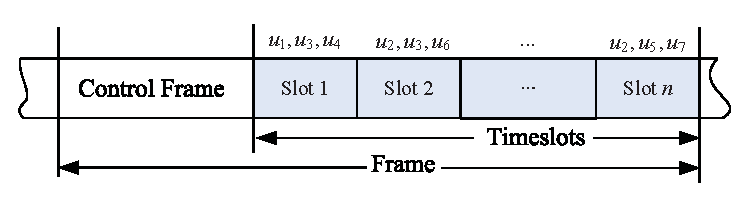
\includegraphics[width=\textwidth]{figures/chapter-5/IssMultiUserComm.eps}
	\caption{多用户复用方式说明图}
	\label{fig:iss-multi-user-comm}
\end{figure}

上图中,帧的前半部分被用来发送信标帧,管理帧等操作,后半部分则用来进行数据的传输。后半部分被划分为了n个时隙,用于用户的时分通信,在每一个时间片上,多个用户可以同时进行数据通信,如时隙1上,用户1,3和4则可以进行数据的传输。
某个用户可以被分配到多个时隙中进行通信,只要此用户在该时隙上不会造成用户间的干扰即可。

这样,当某一次调度完成后,将会形成上图所示灯组的调度结果。之后的所有的帧都将会按照此结果进行灯组的开关和与用户的通信。

\subsection{用户虚拟小区}
由于在该架构下,各灯组可以独立地传输信息,而根据上述提到的独立式组网光通信系统的特征,为了更好地服务用户,系统可以采用用户周边的灯组来共同协作,进行用户数据的传输。考虑到目前光通信灯组的发送角度都较小,且为了尽可能地保障用户连接的可靠性,本系统采用用户可以接收到的所有灯组给用户发送信息。
这里,我们将可以被用户接收到的所有灯组称作为用户的虚拟小区。灯组以虚拟小区的方式为用户提供光通信数据服务。在一个10个用户,36个灯组的场景中,可以通过下图来描述用户的虚拟小区。

\begin{figure}[htbp]
    \centering
	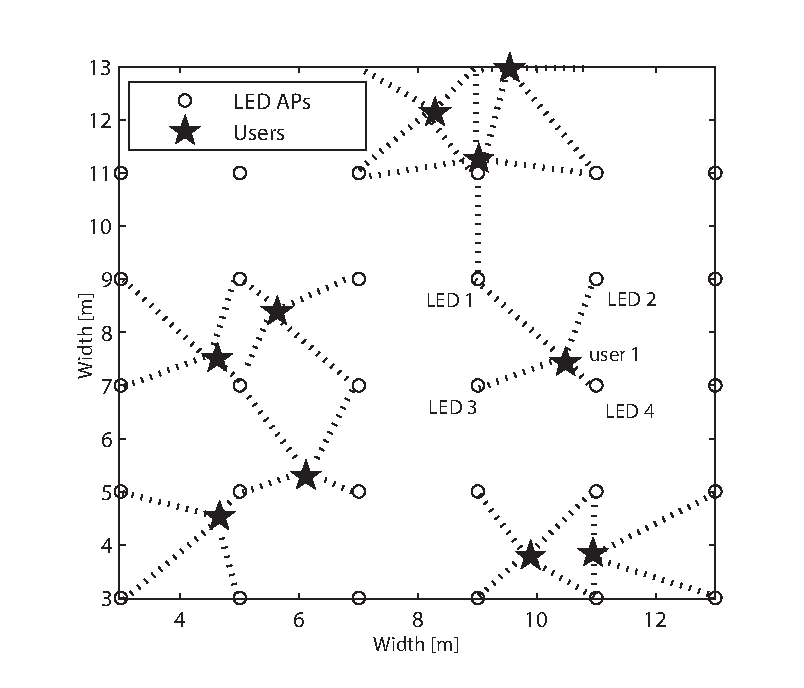
\includegraphics[width=\textwidth]{figures/chapter-5/UserInterference.eps}
	\caption{用户虚拟小区示意图}
	\label{fig:user-interference}
\end{figure}

从上图中,使用星号表示用户的分布情况,使用虚线描绘了各个用户的虚拟小区情况,如LED灯组1,灯组2,灯组3和灯组4将会组成用户1的虚拟小区集合,为该用户服务。同时也可以看到,当两个用户分布较为集中时,其虚拟小区中也就会存在相同的LED灯组,
这也就意味着这两个用户是不能被同时服务到的,必须被分隔在不同的时间片中进行数据传输。具体的用户的干扰问题将在下节描述。

\subsection{用户之间的干扰}
如上所述,当用户的虚拟小区之间存在相同的LED灯组时,则表明用户之间存在相互干扰。本系统为了简化分析,并没有考虑用户之间的干扰的大小,而是设定灯组的调度方案必须能够避免用户之间的干扰。
这样,使用灯组调度算法在每个时隙中选择出来的用户之间必须完全没有相同的LED灯组出现。同样,上述场景下产生的用户间干扰如下图所示。

\begin{figure}[htbp]
    \centering
	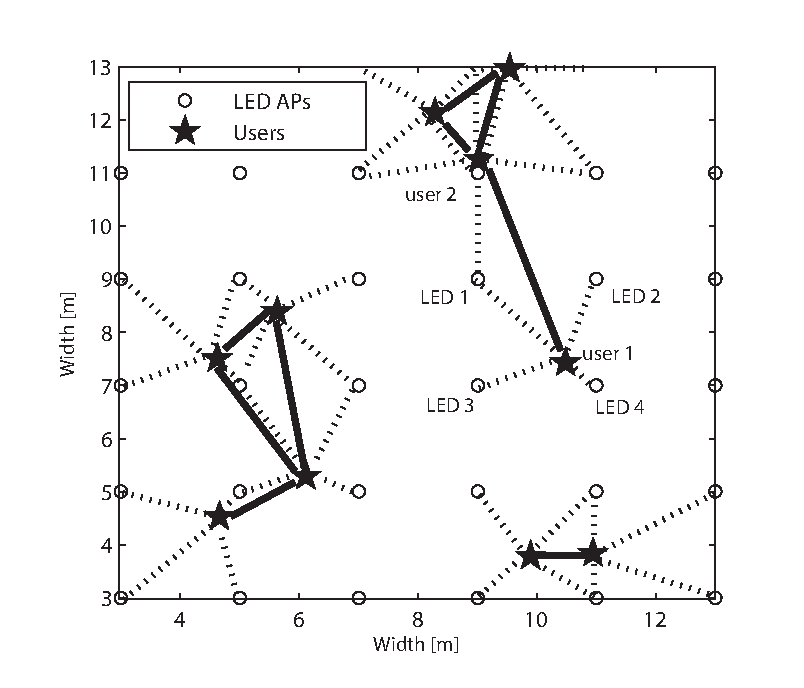
\includegraphics[width=\textwidth]{figures/chapter-5/UserInterferenceShow.eps}
	\caption{用户之间的干扰示意图}
	\label{fig:user-interference-show}
\end{figure}

如上图所示,用户1和用户2的虚拟小区中的灯组集合中都包含LED灯组1,因此,用户1和用户2之间存在用户间干扰,为了避免该干扰的产生,这两个用户就不能被同时服务,所以这两个用户需要被调度到不同的时隙中。

\subsection{图论介绍}
图论是数学中的一个分支,它以图作为研究对象。图论中的图是由若干给定的点及连接两点的线所构成的图形,这种图形通常用来描述某些事物之间的某种特定关系,
用点代表事物,用连接两点的线表示相应两个事物间具有这种关系[]。图论的产生和发展主要经历了如下的几个阶段[]。

第一个阶段是从1736年到19世纪中叶。当时图论的焦点主要是比较流行的迷宫问题和游戏类问题。主要最为出名的是著名数学家欧拉解决的哥尼斯堡七桥问题。
欧拉通过图论的方法描述和论证了该问题。第二个阶段是从19世纪中叶到1936年,该段时期图论的发展仍是以游戏类问题为主,如迷宫问题,博弈问题,棋盘行走问题,其中比较著名的问题有四色问题,Hamilton环游世界问题。
图论发展的第三个阶段是在1936年以后,由于计算机和通信网络的不断发展,使得点对点之间的连通性问题不断出现,从而涌现了如最短路问题,稳定性问题等一系列的图论问题,促进了图论的不断发展。
目前,随着计算机的不断运用,图论已经和计算机科学,电子学,信息论不断地结合,并得到了广泛的应用。

图G可以表示为一个二重组合:

\begin{equation}
    G =  < V,E >
\end{equation}

其中$V$是非空有限集合,它的元素被称为结点,而$E$也是一个非空有限集合,其元素被称为边。某条边$e$也可以看作是一个结点的二重组合$<a,b>$,其中$a$和$b$是属于集合$V$。
如果边$e$是有序的,该边就称为有向边,简称为弧,若边$e$是无序的,该边就称为无向边。

每条边都是无向边的图就被称为无向图,而每条边都是有向边的图就被称为有向图。下图分别展示了一个无向图和一个有向图的实例。

\begin{figure}[htbp]
    \centering
	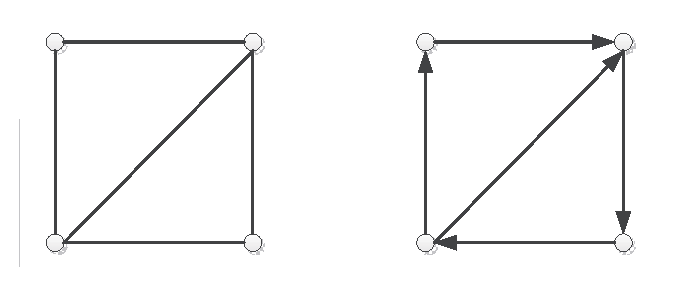
\includegraphics[width=\textwidth]{figures/chapter-5/GraphExample.eps}
	\caption{有向图无向图实例}
	\label{fig:graph-example}
\end{figure}

对于有向图而言,以结点$v$为起点的边数被称为$v$的出度,通常被记为$deg^{+}(v)$,以结点$v$为终点的边数称为$v$的入度,通常被记为$deg^{-}(v)$,而结点$v$的总体度则被定义为上述的入度和出度之和。
对于无向图而言,结点的度则较为简单,就是与该结点相连的所有的边的个数。若所有的结点的度都相等,那么该图就被称为正则图。

给定两个无(有)向图$G=<V, E>$和$G'=<V',E'>$,如果有$V'$包含于$V$且$E'$包含于$E$,则称$G'$是$G$的一个子图。如果此时$G'$不等于$G$,那么$G'$就是$G$的一个真子图。对于一个张图而言,可以生成多个子图。

\section{增量式灯组调度算法}\label{sec:incremental-schdule-scheme}
\subsection{增量式灯组调度算法概述}
灯组的调度需要考虑两个问题,首先是上述的用户优选问题,安排合适的用户在相应的时隙中,利用其虚拟小区中灯组为用户提供服务。在用户的选择时,需要兼顾消除用户之间的干扰和竟可能地增大系统容量。
第二个问题则是用户的移动性问题,当根据当前的所有用户的信息,制定好了最佳的灯组调度策略之后,随着用户的移动,原先的灯组调度策略将有可能不在适合当前用户移动后的场景。
对于第一个问题,我们可以将其看作为一个最优化问题,采用最优化策略来求解。而对于第二个问题,可以采用按照一定频率反复运行灯组调度算法来不断地根据当前场景进行灯组调度。但是这样做,会带来高复杂度和运算量的问题。

本文提出了一种增量式调度算法来解决独立式灯组组网光通信系统下的移动性多用户灯组调度问题,算法主要包含两个部分,全局调度算法和局部调度方法。
其中全局调度算法采用图论的方法对用户位置及用户间干扰进行建模,综合考虑到所有用户的情况,力图达到一个全局最优或者接近最优的系统容量,但是全局调度算法具有复杂度高的缺点。
而局部调度算法则是在全局调度算法结果的基础上,考虑到当前发生移动的用户,采用简单的方案为其重新安排合适的灯组,并协调好与其他灯组之间的关系,在没有过分损失系统容量的情况下适应移动用户的运动,并减低用户的运算量。

增量式调度方案由长时间周期调度的全局算法和短时间周期调度的局部算法组成,即运行一次全局调度,再运行多次局部调度,并重复执行,可以综合两种调度方案的优点,克服只使用全局最优算法导致的运算量大的缺陷,
在获得较好的系统容量的前提下,显著降低系统调度的运算量。下面将会分别介绍两种调度子算法,并详细地对上述的两种子调度算法进行分析。

\subsection{全局调度方法}
全局的调度算法考虑到所有用户当前可使用的灯组情况,以系统容量作为优化目标,通过建立带权重的无向图对该问题进行建模,并提出了比较完善的调度方案。
该算法在分析所有用户信息的基础上,将用户分配到合适的时隙上,消除了用户之间的干扰,并保证了较优的系统容量。

\subsubsection{用户优选问题的建模}
首先需要定义一些系统的参量,如上文所说,在每个用户在通信时,为了获得可靠的通信效果,可以使用虚拟小区为其提供通信协作,因此这里定义为用户$u_{i}$服务的虚拟小区为$VC_{i}$。

为了最大化系统的容量,本文定义了以下的系统效用函数:

\begin{equation}
    \sum\limits_{i = 1}^K {{U_i}({{\bar r}_{i,k}})}
\end{equation}

其中,$U_i()$是一个用于衡量用户$u_{i}$吞吐量的效用函数,${\bar r}_{i,k}$是用户$u_{i}$在时隙$i$前计算出的平均速率,定义为:

\begin{equation}
    {\bar r_{i,k}} = (1 - \frac{1}{{{T_c}}}){\bar r_{i,k - 1}} + \frac{1}{{{T_c}}}{r_{i,k - 1}}
\end{equation}

其中,$T_{c}$表示为比例系数,该值可以决定在前一个时隙中用户的速率占用户的平均速率的比例。

假设第$k$个时隙中的所有用户可达速率集合的向量定义为

\begin{equation}
    \overrightarrow {{r_k}}  = {[{r_{1,k}},{r_{2,k}},...,{r_{K,k}}]^T}
\end{equation}

其中,$r_{i,k}$指的是在时隙$k$上用户$u_{i}$可以获得的速率。根据基于梯度的调度框架[],调度的主要目标就是在梯度的方向上选择合适的$\overrightarrow {{r_k}}$,因此,最优化系统容量的问题转化为:

\begin{equation}
    \max \sum\limits_{i = 1}^K {{{U'}_i}(\overline {{r_{i,k}}} )} {r_{i,k}}
\end{equation}

本文采用了一个较为典型的效用函数,如下所示:

\begin{equation}
    {U_i}(\overline {r}_{i,k}) =
    \begin{cases}
        \alpha^{-1} {\overline {r}_{i,k}}^\alpha ,  & \alpha \le 1 \mbox{and} \alpha \ne 0 \\
        log(\overline {r}_{i,k}),                   & \alpha = 0
    \end{cases}
\end{equation}

其中,$\alpha$表示公平系数,代表用户间可达速率的公平程度,将()代入(),于是问题也就被转化为:

\begin{equation}
    \max \sum\limits_{i = 1}^K {{{\overline {r}_{i,k} }^{\alpha  - 1}}{r_{i,k}}}
\end{equation}

可见,当前的目标函数将会受到参数$\alpha$的影响,不同的$\alpha$值将代表着不同的公平性,为了满足系统的要求,这里较为简单地设置$\alpha$为0,
这样,目标函数就转变为:

\begin{equation}
    \max \sum\limits_{i = 1}^K {\frac{{{r_{i,k}}}}{{\overline {r}_{i,k} }}}
\end{equation}

上述的目标函数则是调度算法在每个时隙选择合适的用户时需要考虑的目标,同时为了防止用户之间干扰的产生,需要保证每个时隙中的用户之间没有公用的灯组,
所以对于上述的目标函数,还需要引入一定的约束条件,时隙间用户不存在干扰,各用户的虚拟小区间不存在公共的灯组等,所以系统的优化模型就转变为:

\begin{equation}
    \max \sum_{i=1}^{K}\frac{r_{i,k}}{\overline{r}_{i,k}} \\
    s.t.\; I_{i} = 0,\; i=1,...,K \\
        VC_{i} \cap VC_{j} = \emptyset  i,j= 1,...,K and i \ne j  \\
        \bigcup_{i = 1}^K V{C_i} \subseteq A
\end{equation}

其中,$I_{i}$代表用户 接收到的干扰信号,集合$A$代表所有的灯组集。

对于$r_{i,k}$,可以用香农公式展开。$r_{i,k}$与用户$u_{i}$在$k$时刻的接收信号功率有关,而由于系统中各个灯组会周期性地发送信标帧来使用户获得当前的灯组信息,
而且信标帧发送的周期较短,两次信标帧之间用户几乎不会发生移动,因此,用户侧可以采用上一次接收到的信标帧的接收功率来近似表示用户当前时隙的接收信号,即

\begin{equation}
    {h_{i,j}}{P_{ot}} \approx {P_{recvj}}
\end{equation}

最后,将$r_{i,k}$按公式展开并带入公式(),可以得到用户优选的系统最优化模型:

\begin{equation}
    \max \sum_{i=1}^{K}\frac{log_{2}(1+\frac{{\sum_{LA_{j} VC_{i}}RP_{recvj}}^2}{I^2+\delta^2})}{\overline{r}_{i,k}} \\
    s.t.\; I_{i} = 0,\; i=1,...,K \\
        VC_{i} \cap VC_{j} = \emptyset  i,j= 1,...,K and i \ne j  \\
        \bigcup_{i = 1}^K V{C_i} \subseteq A
\end{equation}

\subsubsection{系统模型的解决}
针对上述的最优化问题,因为离散问题的全局最优化问题很难直接解决,本文运用图论的方法将该问题使用图论进行了重新的描述,并采用相应的算法对该图论问题进行了求解。

由于用户在灯组下的布局很容易用一个无向图进行表示,同时用户之间的干扰也可以用图论中两个节点是否存在连接线来表示,所以,本文采用了一个带权重的无向图来对上述最优化问题进行了重新的建模。
首先,需要可以定义一些参数,$G(V,E)$表示建立的用户干扰图,$V(G)$表示图G中的顶点集,$E(G)$表示图$G$中的边集。$v_{i}$表示在点集$V_{G}$中的一个节点,$N(v_{i})$表示该节点的相邻节点集,
$d(v_{i})$表示节点$v_{i}$的度,也就是相邻节点集$N(v_{i})$中节点的个数。在用户图上对于每个节点增加一个权重值,就构成了带权重的无向图$G^{w}(V,E)$。干扰图中的顶点$v_{i}$代表场景中的某一个用户,
而干扰图中的在边则依据用户之间是否存在干扰,当两个用户之间存在干扰时,图中的两个顶点之间也就存在一条边,否则两点之间没有连线。同时根据前一节分析的调度目标函数,
这里按照式()在时隙$k$时设置干扰图中各个顶点的权重值。

\begin{equation}
    {p_{i,k}} = \frac{{{r_{i,k}}}}{{\overline {r}_{i,k} }}
\end{equation}

对上述给出的多用户在多个灯组下的通信场景按照上述的图论的方法进行建模,可以得到描述该系统用户之间干扰的干扰图如下:

\begin{figure}[htbp]
    \centering
	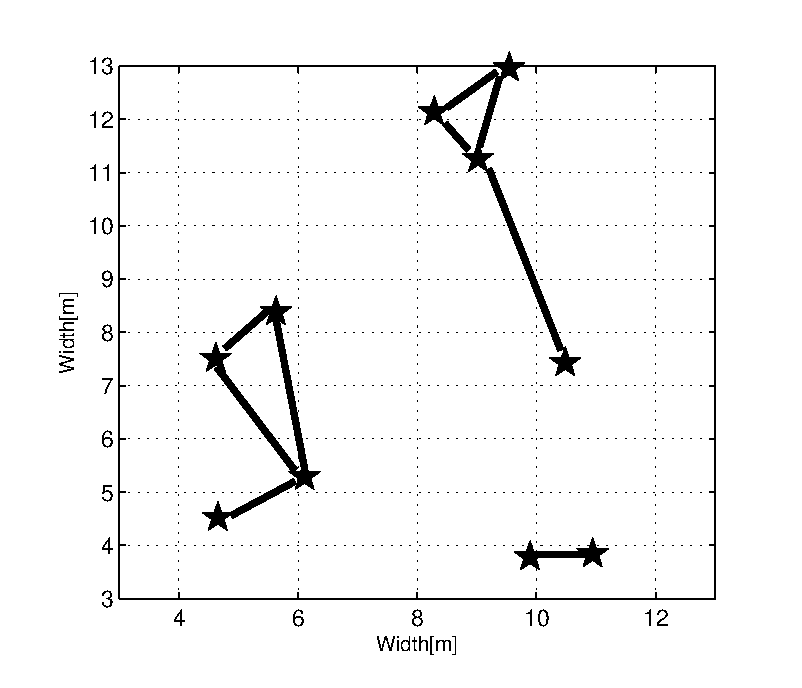
\includegraphics[width=\textwidth]{figures/chapter-5/InterferenceGraph.eps}
	\caption{用户干扰图}
	\label{fig:interference-graph}
\end{figure}

图中,五角星则表示的是场景中的用户,之间的连接线表示的是用户之间存在干扰。例如,用户1和用户4之间是存在干扰的,在同一个时隙下不能被同时选中,用户1和用户6之间是不存在干扰的,可以同时进行数据通信。

经过上述图论的描述之后,问题被转变为如何在这个带权重的无向图中找到一组顶点,使得任意两个顶点之间没有边,同时该组顶点的权重值之和最大。该组顶点的集合可以被记为最大权重顶点集。参考文献[],使用了贪心算法可以很好地解决这个问题。
在使用贪心算法中,依据的思想是如果图中某一顶点的度越大,该顶点干扰的其他用户也就越多,因此该顶点也就越不应该被选中。所以系统以$p_{i,k}^{'}=\frac{p_{i,k}}{d(v_{i}+1)}$作为标准来进行某一时隙激活用户的选取。每次选取$p_{i,k}^{'}$值最大的顶点,
并将该顶点和图中与该顶点相邻的顶点集合去掉,重复上述过程,直到图中的顶点全部被选择完成为止。具体的基于图论的灯组选择算法为:

%
%算法图
%

上述的基于图论的灯组选择算法可以保证在一个时隙中选择出合适用户,但为了保证每个用户在此次调度中都能够被服务到,本文使用了比例公平算法,从而保证能在多个时隙中服务完成所有的用户。

比例公平算法的目的是,为了保证在上一个时隙被服务过的用户就只能获得较小的权重,而上一时刻没有被服务的用户可以获得较高的权重,从而,可以将所有用户较好地安排在多个时隙中。
因此,系统在调度完成一个时隙之后,会按照式()重新更新当前的用户图上各节点的权重,然后再次按照上述基于图论的灯组选择算法选择另外一组用户,直到所有的用户都被服务过。

根据上述的描述,全局调度算法可以总结为以下步骤:

\begin{enumerate}
    \item 各灯组每隔一段时间会定时发出的beacon信息,用户将会记录下beacon信息的接收功率和发送的灯组号,并上报给光通信中的调度器;
    \item 调度器利用上报的信息形成用户之间的干扰图,并为各阶段计算出相应的权重值;
    \item 根据干扰图各节点的权重,依据贪心算法分析出当前时隙可被激活的用户;
    \item 更新干扰图中的节点权重信息;
    \item 重复(3)直到所有的用户均被服务过;
    \item 得到灯组的全局调度结果。
\end{enumerate}

\subsection{全局调度方法}
由于场景中用户的移动性,使得全局调度产生的灯组调度方案在一段时间后将不再适应于用户当前的位置,具体点说,则是用户的移动导致了用户当前的虚拟小区将不再是全局调度时刻的虚拟小区。
因此,系统采用局部调度方法根据当前用户上报的信息,选择出需要进行局部调整的用户,采用了回溯算法,为移动用户更新合适的灯组资源,进而保障通信中用户的移动性。局部调度算法可以按照以下三部分进行。

\subsubsection{运动用户集合}
运动用户集合的划分主要通过用户的上报的灯组信标帧的情况进行划分,由于系统的每个灯组在超帧时间内都会发送信标帧来广播自身的信息,所以当用户接收到周期性发送的灯组信标帧之后,就会将接收到的灯组的编号反馈给系统调度器,该组灯组的编号也就是当前可以为该用户提供服务的灯组集合。
当调度器一段时间内统计到某个用户的可用灯组信息发生了变化后,就将该用户放入到运动用户集合(moving user set,MUS)中,等待进行后续的调度操作。

\subsubsection{子图内用户间干扰}
局部调度是在全局调度的基础上进行的,当全局调度完成之后,系统将会获得全局调度的调度信息,如具体时隙中使用哪些灯组服务哪些用户。因此,当已知了移动用户的集合之后,可以同样从全局调度中的图论的角度出发。
全局调度会把所有的用户划分在若干个调度子图中,即每一个调度的时隙中的用户及其之间的关系形成一个调度子图。在子图中,由于全局调度完成后会保证子图中的用户之间是没有干扰的,因此调度完成之后的子图中各个结点之间是没有连线的,
同样,上述实例中进行了全局调度后的子图划分如下所示。

\begin{figure}[htbp]
    \centering
    \subfloat[第一个子图]{
        \label{fig:slot-1-before-move}
        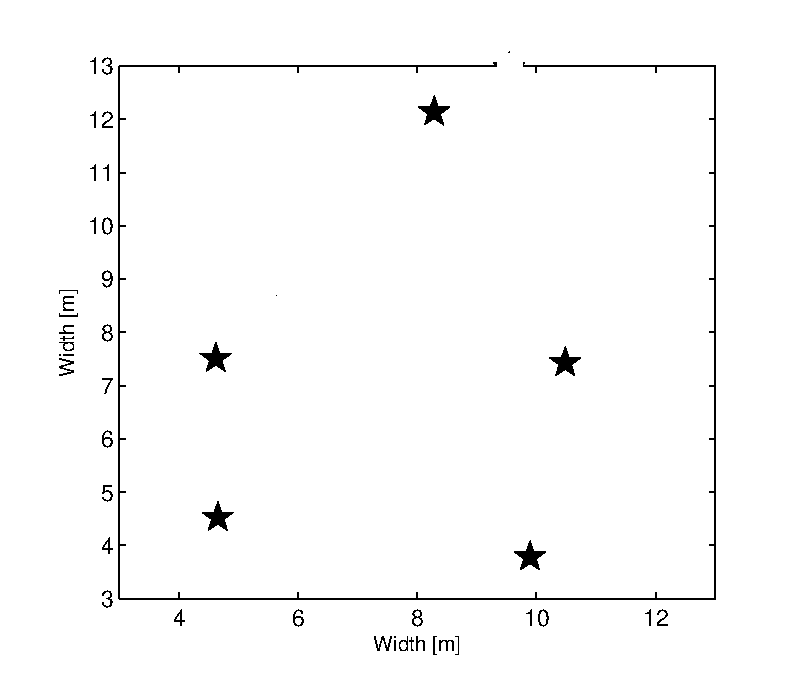
\includegraphics[width=0.5\textwidth]{figures/chapter-5/UserBeforeMove1.eps}
    }
    \subfloat[第二个子图]{
        \label{fig:slot-2-before-move}
        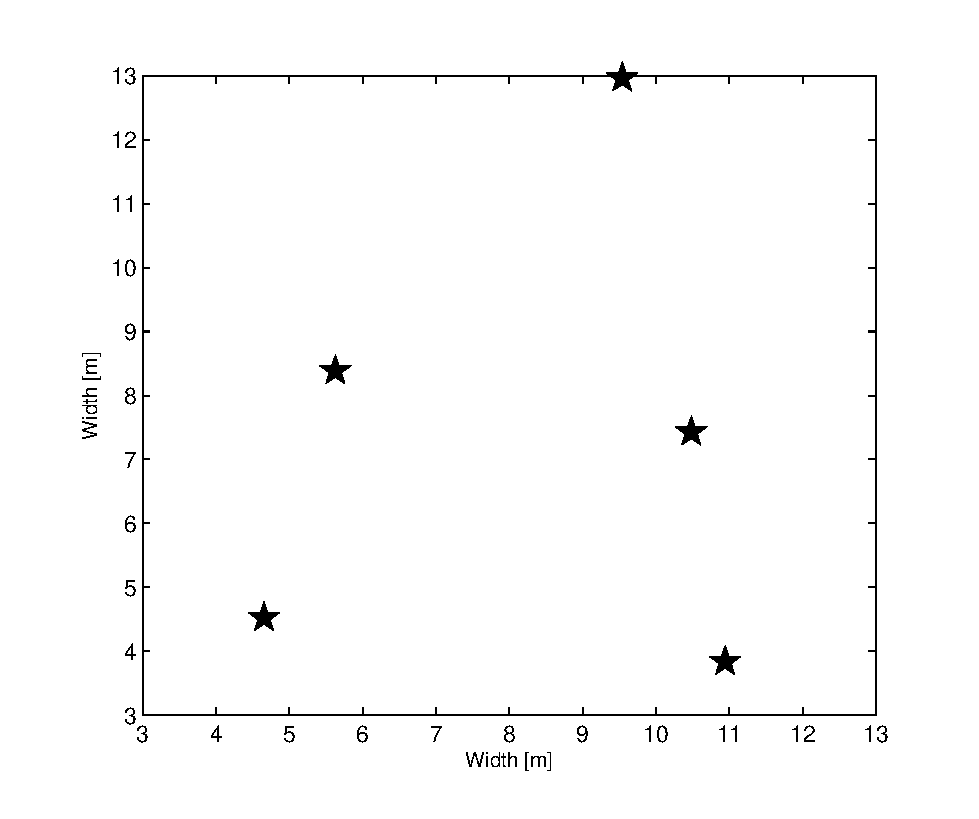
\includegraphics[width=0.5\textwidth]{figures/chapter-5/UserBeforeMove2.eps}
    }
    \subfloat[第三个子图]{
        \label{fig:slot-3-before-move}
        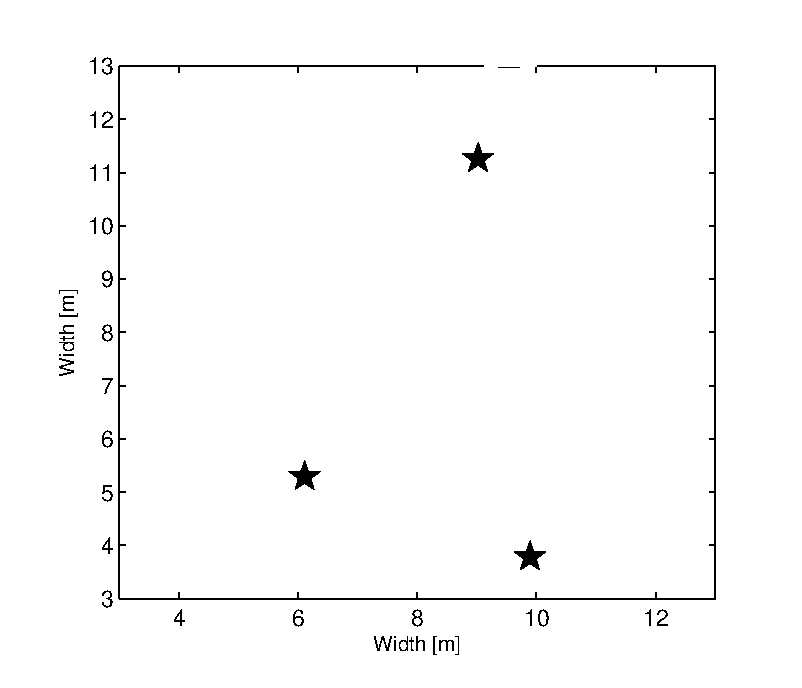
\includegraphics[width=0.5\textwidth]{figures/chapter-5/UserBeforeMove3.eps}
    }
    \caption{用于运动前的子图情况}
    \label{fig:slot-before-user-move}
\end{figure}

在一段时间之后,当用户位置发生了改变,会使得用户之间再次形成干扰,这样的干扰当然可以再一次使用全局调度来解决,但如上分析,那将会耗费较大的调度时间。这里首先可以充分利用全局调度带来的多子图的优越性,全局调度能够将距离较近,容易形成干扰的两个用户分隔在不同的时隙中,
从而使得用户移动带来的影响分散到各个子图中。因此,当用户移动后,我们只需要去关注和解决子图中的用户间干扰即可。如下图所示,当用户7发生了移动,则会在子图1和子图3中发生用户间的干扰,局部调度就是要去解决这两个子图中的干扰即可。具体的子图中干扰解决方案将在下节中进行讨论。

\begin{figure}[htbp]
    \centering
    \subfloat[第一个子图]{
        \label{fig:slot-1-after-move}
        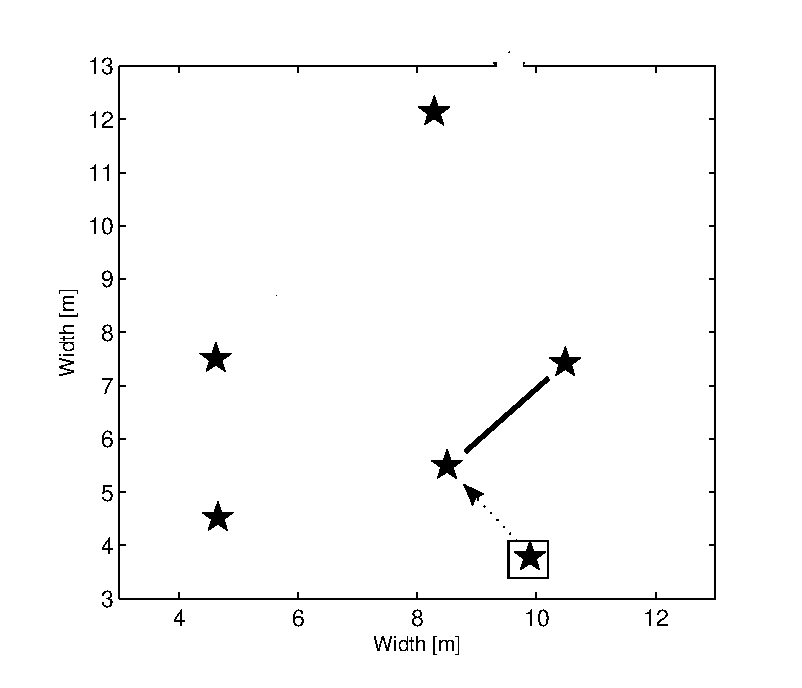
\includegraphics[width=0.5\textwidth]{figures/chapter-5/UserAfterMove1.eps}
    }
    \subfloat[第二个子图]{
        \label{fig:slot-2-after-move}
        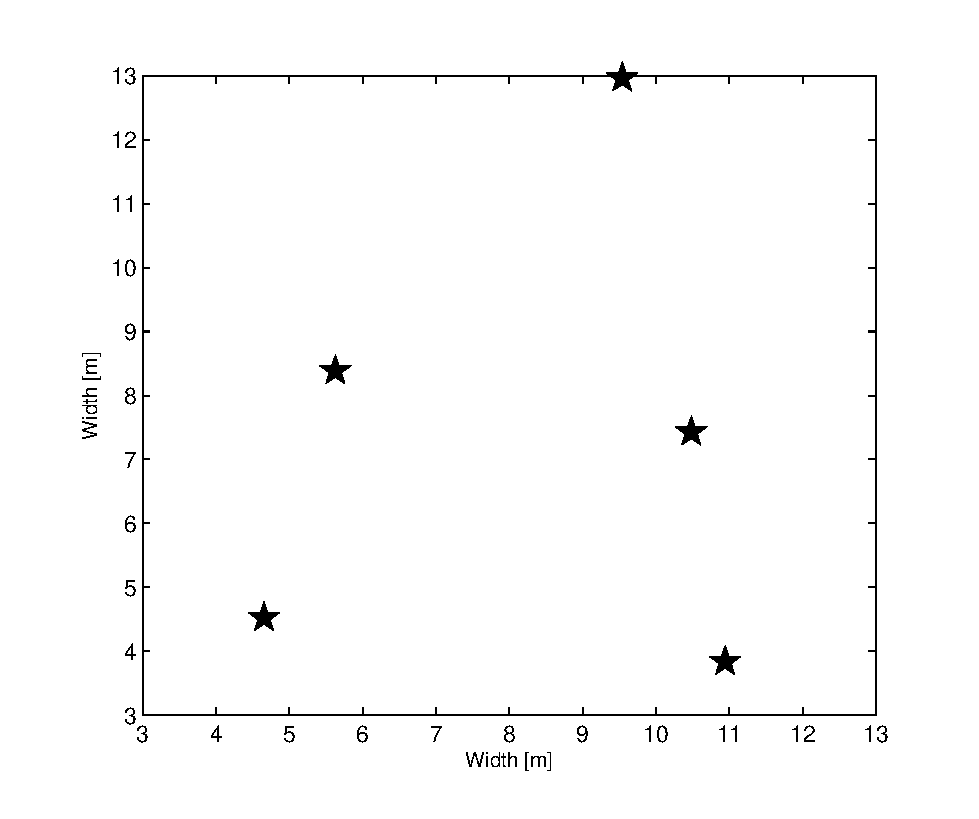
\includegraphics[width=0.5\textwidth]{figures/chapter-5/UserAfterMove2.eps}
    }
    \subfloat[第三个子图]{
        \label{fig:slot-3-after-move}
        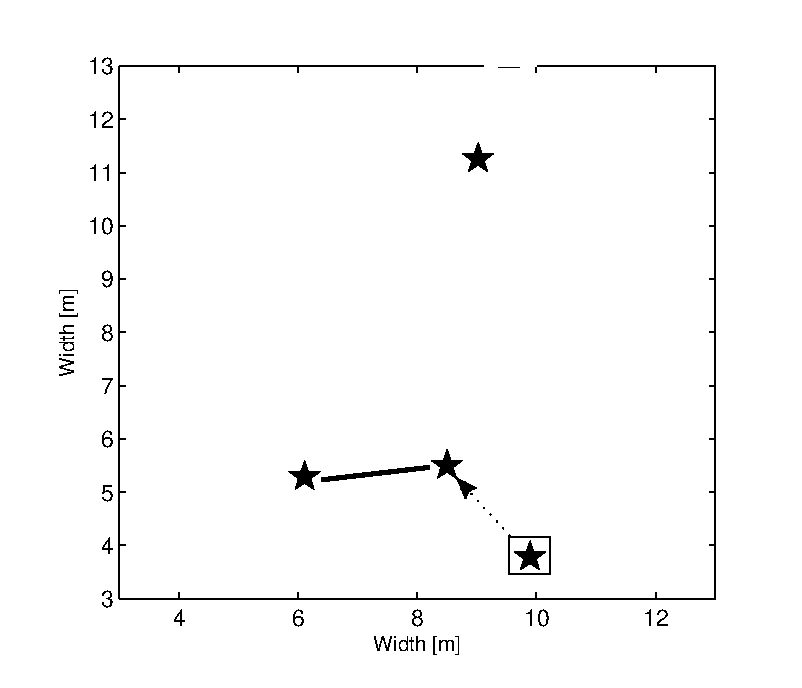
\includegraphics[width=0.5\textwidth]{figures/chapter-5/UserAfterMove3.eps}
    }
    \caption{用于运动前的子图情况}
    \label{fig:slot-after-user-move}
\end{figure}

\subsubsection{移动用户最优时隙选择}
在考虑如何处理移动用户可能带来的用户间干扰前,可以先考虑一下如下方面问题。首先,由于在全局调度后某个用户有可能会在多个子图中出现,它的移动也可能引起多个子图内的用户间干扰。其次,某个用户的移动可能会导致该用户适合于原先不存在该用户的子图,因此,对于运动用户的调度,
不应该仅仅着眼于它当前分配的子图中,也应该考虑其在其他子图中出现的可能性。

在解决子图干扰时,所有非运动用户仍然分配在全局调度所分配的子图中,系统通过对运动用户集合中的用户进行调度,在兼顾系统容量的同时,保证运动用户可以获得较好的调度灯组,完成系统的局部调度,这种方式也将大大减小局部调度所需要的运算量。

这里,可以分两种情况来讨论用户移动在全局调度基础上对系统造成的影响。一种情况是某个用户的移动在子图内都没有造成子图中用户间的干扰,对于这种情况,系统可以直接将全局调度中为该用户服务的灯组更改为该用户当前的虚拟小区中的灯组即可。另一种情况则是当用户的移动在某一个子图中造成了子图中用户间的干扰,
这里就需要对该用户的可存在性进行判决。若要使得用户可以存在于子图中,就必须将用户放入子图中时,关闭该时隙内所使用的所有灯组中与该用户虚拟小区中相同的LED灯组,这种关闭相同灯组的方式可以消除用户间的干扰,但是当移动用户与它所在时隙中其他用户的LED灯组的重复率过高时,会严重降低系统容量。
因此,为了保障系统容量,对于移动用户在子图中可存在性判决的依据是用户在子图中的存在将导致子图的容量值的变化。系统定义的一个子图容量变化值如下式

\begin{equation}
    \Delta {C_{ij}} = {C_{aij}} - {C_{bij}}
\end{equation}

其中,$\Delta {C_{ij}}$表示的是在子图$SG_{i}$中添加用户$u_{j}$后引起的子图容量的变化,$C_{bij}$和$C_{aij}$表示的是在加入用户$u_{j}$之前和之后的子图的系统容量,定义子图k中的系统容量计算公式为:

\begin{equation}
    {C_k} = \sum\limits_{i = 1}^K {{{\log }_2}(1 + \frac{{{{(\sum\limits_{L{A_j} \in V{C_i}} {R{P_{recvj}}} )}^2}}}{N}))} {\kern 1pt} {\kern 1pt} {\kern 1pt} {\kern 1pt} {\kern 1pt} {\kern 1pt} {\kern 1pt} {\kern 1pt} {\kern 1pt} {\kern 1pt} {\kern 1pt} {\kern 1pt} {u_i} \in A{U_k}
\end{equation}

其中$AU_{k}$表示的是子图中被激活的用户。

当$\Delta {C_{ij}}$为正时,则表明把运动用户存在在此子图中时,对获得系统容量的增加有利,当该值为负时,则表明用户在此子图的存在,
将会对其他用户造成较为严重的干扰,不能保证很好的系统容量,该用户不应该分配在该子图中。

于是,根据上述的算法和移动用户自身的特点,对运动用户集合中的每个用户,判断其干扰产生的影响,并为其选择合适的调度灯组,
从而获得较优的灯组调度结果。综上所述,局部调度主要分为如下几个步骤:

\begin{enumerate}
    \item 根据用户上报信息,根据灯组集的改变情况,组成局部调度用户集;
    \item 调度器利用上报的信息形成用户之间的干扰图,并为各阶段计算出相应的权重值;
    \item 根据干扰图各节点的权重,依据贪心算法分析出当前时隙可被激活的用户;
    \item 更新干扰图中的节点权重信息;
    \item 重复(3)直到所有的用户均被服务过;
    \item 得到灯组的全局调度结果。
\end{enumerate}

\section{仿真实验及结果分析}\label{sec:iss-simulatioon-result}
为了对提出的增量调度的算法进行分析,本文在NS2平台上进行了独立式灯组光通信场景模型的建立和仿真,模拟了用户在用户过程各种灯组的调度过程。仿真中的场景和上述的实例一样,设置了6*6个灯组和10个用户,灯组被规则地分散放置在房间内,
用户的位置则是随机均匀分布在用户接收平面上,仿真中需要设定具体的光通信参数,如灯组的属性,干扰的具体参数等,其具体数值列表如下:

\begin{table}[htbp]
    \caption{独立式灯组调度仿真参数表}
    \label{tab:iss-simulation-param}
    \centering
    \begin{tabular}{llll}
        \toprule
        参数     & 数值 & 参数 & 数值 \\
        \midrule
        d        & 2m                & h           & 2.2m \\
        A        & $0.785mm^{2}$       & $P_{ot}$      & $3600*30mw$ \\
        $T_{k}$    & 300k              & $\Phi_{1/2}$  & 70deg. \\
        $\eta_{c}$ & $1.12*10^{-6}F/m^2$ & R           & $0.54A/W$\\
        G        & 10                & $I_{bg}$      & $5.1*10^{-3}A$ \\
        $\Gamma$   & 1.5               & $I_{2}$       & 0.562 \\
        $I_{3}$    & 0.0868            & B           & 100MHz \\
        $g_m$      & 0.03S \\
        \bottomrule
    \end{tabular}
\end{table}

为了考察本文的增量式调度算法对移动用户和系统性能的影响,在仿真中主要从移动用户的接收信噪比的情况和调度对系统容量的影响来进行系统的分析。

这里定义用户的接收信噪比为:

\begin{equation}
    SNR = \frac{{\sum\limits_{i = 1}^N {{{(\sum\limits_{A{P_j} \in V{C_i}} {{h_{ij}}{P_{ot}}R} )}^2}} }}{N}
\end{equation}

其中,$N$表示的是该用户虚拟小区中的灯组的个数。而在一个时隙中用户的系统容量为:

\begin{equation}
    capacit{y_m} = \sum\limits_{i = 1}^K {{{\log }_2}(1 + \frac{{{{(\sum\limits_{A{P_j} \in V{C_i}} {{h_{ij}}{P_{ot}}R} )}^2}}}{N})}
\end{equation}

其中$K$表示该时隙中的用户的个数。则在整个调度过程中系统的总的系统容量为:

\begin{equation}
    capacity = \sum\limits_{m = 1}^M {capacit{y_m}}
\end{equation}

在仿真中,为了检验本文所提出的增量式调度算法的性能,设置了两种对比算法,即高频度的全局调度和低频度的全局调度,其中高频度的全局调度算法由于能够及时根据所有用户的位置进行灯组调度,可以看作为接近最优系统容量的调度方法。而把低频度的全局调度的调度时间间隔设置为10s,和采用了间隔10s调度一次的全局调度和间隔1s调度一次的局部调度相结合的增量式调度方法相比,
低频度的全局调度算法可以看作为只是用了全局调度而没有使用局部调度算法的增量式调度。

\subsection{不同的用户移动速度对用户SNR分布的影响}
仿真中,将10个用户初始随机地分布在接收平面上,首先使得一个用户进行移动,为了检查算法对移动用户的支持,本文采用了cdf曲线来考察用户的接收信噪比的分布情况。分别仿真了用户在1m/s情况下的高频度全局调度和低频度全局调度的用户信噪比分布情况和用户在0.5m/s,1m/s和2m/s下使用本文提出的增量式调度方法的接收信噪比分布。
其仿真结果如下图所示。

\begin{figure}[htbp]
    \centering
	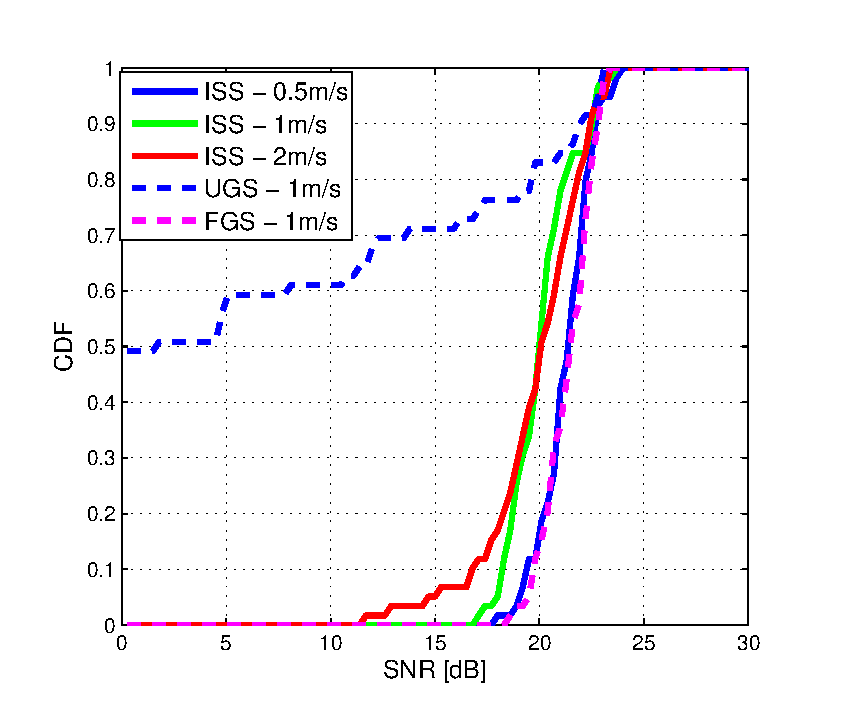
\includegraphics[width=\textwidth]{figures/chapter-5/Speed2Snr.eps}
	\caption{用户移动速度对用户SNR分布的影响}
	\label{fig:speed-2-snr}
\end{figure}

从上图中可以看出,短频度的全局调度算法由于不能很好地对用户的移动性提供支持,当用户运动后,由于系统没有能够及时地进行调度,导致为该用户服务的灯组还是原先设定的LED灯组,从而导致系统的接收信噪比的取值较为分散,在0-24dB均有分布。而与之相比,由于高频度的全局调度能够实时地进行用户LED灯组的调度,
所以也就能确保用户获得很好的信噪比的分布,其用户信噪比都集中分布在18-23dB附近。而本文提出的增量式调度算法,其接收信噪比远好于低频度的全局调度,并当用户的速率较低时,其信噪比分布接近于高频度的全局调度的分布。同时我们可以看到,当用户的移动速率变高时,用户的信噪比cdf分布也就越宽。
这是因为,随着用户的移动速率的逐渐增加,使得移动用户移动到接收信号差的区域的几率增加,从而导致用户低信噪比出现的概率增加。图中的数据表明,在正常的用户移动速率下,用户的信噪比分布较为平稳,能基本满足高速数据通信的需求。

\subsection{不同的接收视场角对用户SNR分布的影响}
由于用户的接收视场角对系统的调度有着重要的影响,不同的接收视场角使得用户的虚拟小区中灯组集的差距较大,也导致不同的用户间干扰的产生。
因此,本文仿真了接收视场角在40度,45度,50度和55度这四种情况下,移动用户的接收信噪比的cdf分布情况,其仿真结果如下图所示:

\begin{figure}[htbp]
    \centering
	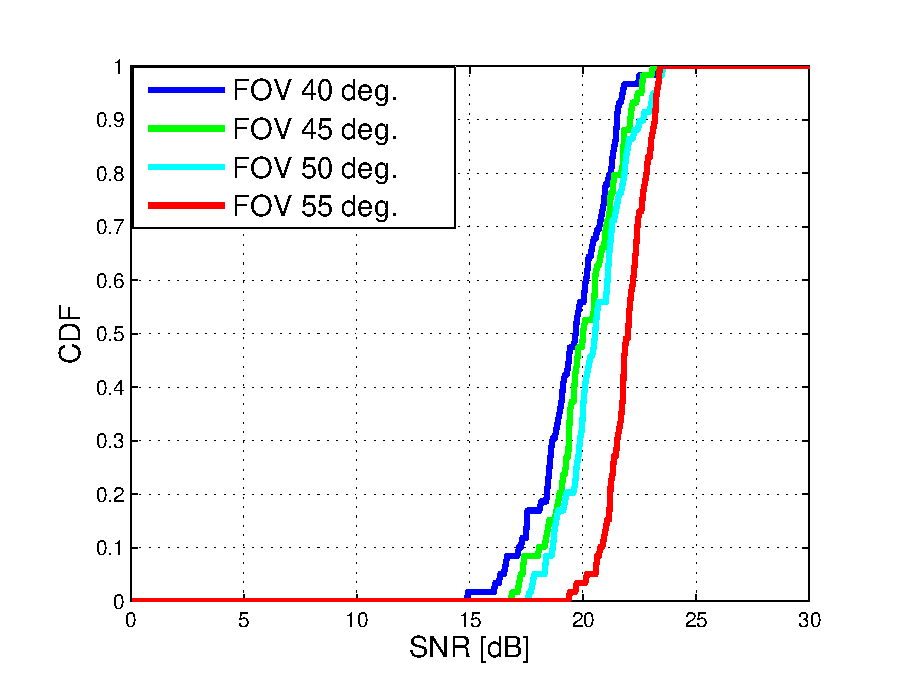
\includegraphics[width=\textwidth]{figures/chapter-5/Fov2Snr.eps}
	\caption{接收视场角对用户SNR分布的影响}
	\label{fig:Fov-2-Snr}
\end{figure}

从图中可以看到,用户的接收视场角对于用户的接收功率的影响较大。随着用户的接收视场角的增大,其信噪比也就越高。这是因为,$FOV$的增加,将会使得可以为该用户服务的灯组的个数也就随之增多,这样对于单个用户来说,其接收信噪比也就增大了,
但是,FOV的增加将会导致用户的虚拟小区的重叠灯组的增多,也就意味着用户间的干扰增加,这样,在进行增量式调度中的全局调度时,就会需要更多的时隙才能将所有用户服务完,也会给后续的局部调度增加复杂度。因此,在本文的算法中,可以在满足用户的信噪比需求的前提下,尽可能选择较低的FOV值。

\subsection{不同的用户数对各调度算法下系统容量的影响}
在室内可见光通信中,用户的规模对系统的调度有着至关重要的影响。为了讨论在不同的用户数的情况下,本文的调度算法对系统性能的影响,进行了如下的仿真。
在仿真中,同样设置场景中存在一个用户进行随机移动,其他用户不运动,并调整不同的用户数量进行仿真,仿真结果如下图所示。

\begin{figure}[htbp]
    \centering
	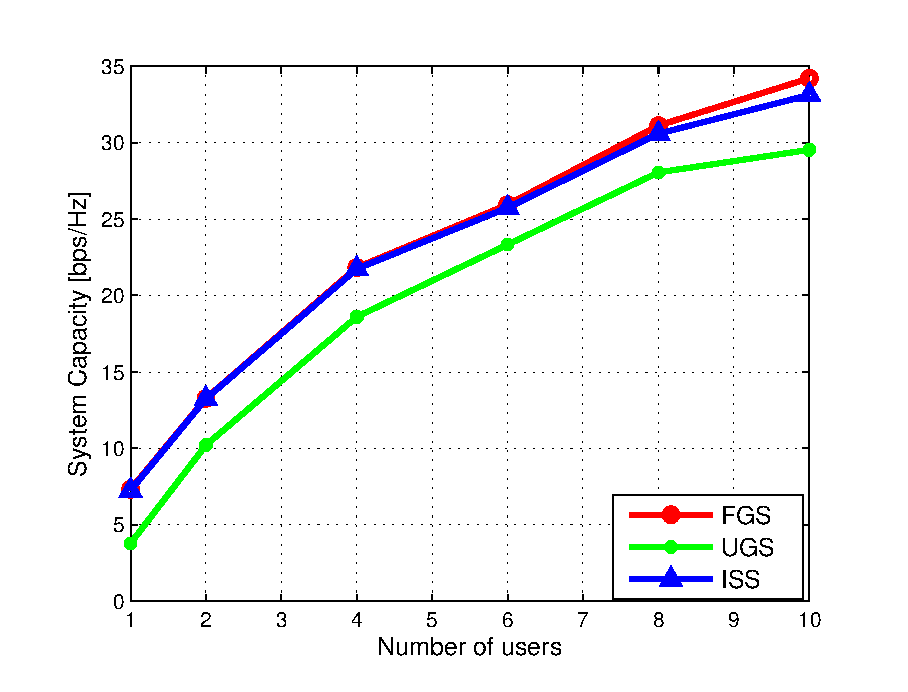
\includegraphics[width=\textwidth]{figures/chapter-5/Usernum2Capacity.eps}
	\caption{用户数对系统容量的影响}
	\label{fig:usernum-2-capacity}
\end{figure}

从图中可以看出,显然随着用户数的不断增加,系统的容量值也不断提高。在当前仿真的一个用户运动的情况下,本文提出的增量式调度算法的系统容量的指标非常贴近于高频度的全局调度算法得到的系统容量曲线。这是因为,本文提出的增量式调度算法不管是在全局调度阶段还是在增量式调度阶段,都很重视对系统的系统容量的影响,
系统容量也是调度算法优化的一个重要指标,在局部调度阶段,虽然用户间的干扰的消除会降低系统的容量,但其对系统容量的影响也是被控制在很小的范围内。因此,本文所提出的增量式调度算法拥有很好的系统容量性能。而低频度的全局调度算法与之相比,在系统容量方面与上述两种算法有差距很大。这是因为进行低频全局调度后,
调度周期内的用户通信质量并不是得以保证,移动中的用户很有可能就会移动出原有的灯组调度范围中,从而带来整体通信性能的下降。上述仿真中假设的是单个用户运动,若场景中存在多个用户运动时,在不同的用户数下系统容量的区别将会更加明显,而由于增量式调度算法中含有针对于移动用户的局部调度算法,因此其调度性能还是可以得到保证的,
具体针对多移动用户的仿真将在下文中详细分析。

\subsection{不同的移动用户数对各调度算法下系统容量的影响}
上述的仿真只提供了一个移动用户的场景,而保障多个用户的移动性时本文算法研究的重要方向,为了研究算法在不同移动用户数目下的系统性能,
本文分别使用三种调度算法,在总的用户数目为10,移动用户的数目分别设定为0到10的情况下,进行了仿真研究。得到的仿真结果如下图所示:

\begin{figure}[htbp]
    \centering
	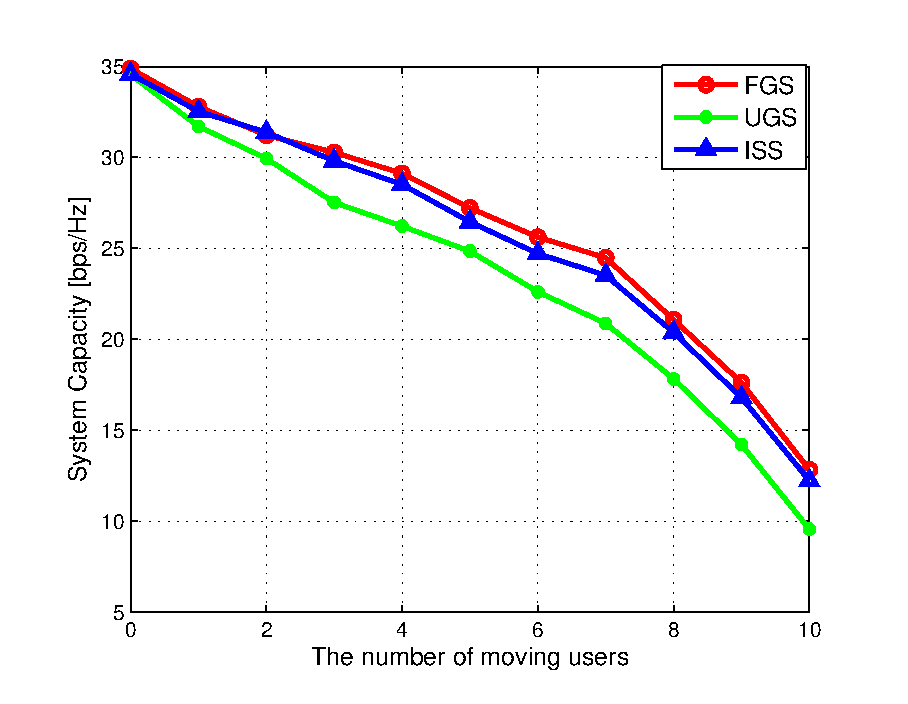
\includegraphics[width=\textwidth]{figures/chapter-5/MovingUserNum2Capacity.eps}
	\caption{移动用户数对系统容量的影响}
	\label{fig:moving-user-num-2-capacity}
\end{figure}

从上图可知,随着移动用户数目的不断增加,三种调度算法的系统容量都呈现不断下降的趋势,这是因为用户移动会导致用户的平均接收信噪比降低,进而影响到整体系统的速率。其中最上面的曲线为采用高频度全局调度的系统容量结果,
因为高频度的全局调度会最大限度得保障系统的所有用户的调度结果最优,使得系统性能接近于理论最优值,所以其系统容量的表现是最好的。低频度的全局调度由于其调度周期的局限性,在多个用户移动的情况下,其系统性能的差距变得非常明显,远低于其他两种算法。
而增量式调度算法由于在局部调度阶段充分考虑到移动用户对系统容量的影响,并为其进行了较优的灯组调度,从而使得在多个移动用户的情况下,增量式调度算法的表现仍然能非常地接近于类似最佳表现的全局调度,也远优于低频度的全局调度。
这说明本文提出的增量式调度算法能够适应存在多个移动用户的调度场景,并能达到较为理想的系统性能要求。

\subsection{不同的移动用户数对各调度算法下复杂度的影响}
在室内可见光通信系统中,对系统调度算法进行分析时,除了对算法的整体调度性能进行分析之外,还需要考虑算法在调度复杂度上的表现。
良好的调度算法应该具有较低的复杂度和较好的硬件可实现性,因此为了比较以上三种算法在算法复杂度上的差异,
本文通过仿真比较了三种算法的总的运算时间。这里的总的运算时间是指在一次仿真中调度算法所使用的平均运算时间。仿真时的参数设置和上一节的设置一样,仿真后的结果如下图所示。

\begin{figure}[htbp]
    \centering
	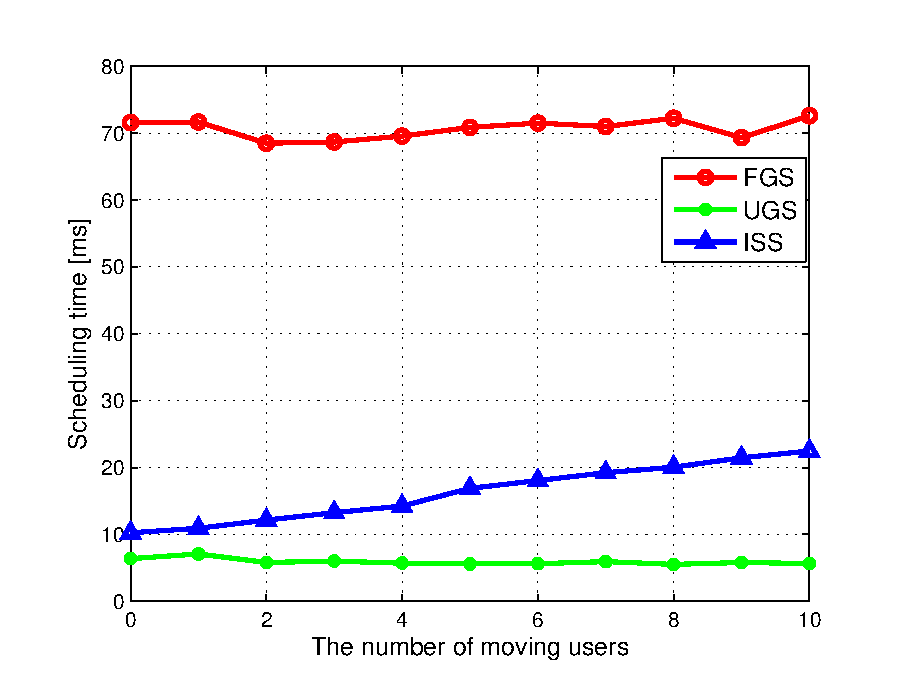
\includegraphics[width=\textwidth]{figures/chapter-5/MovingUserNum2Complexity.eps}
	\caption{移动用户数对调度复杂度的影响}
	\label{fig:moving-user-num-2-complexity}
\end{figure}

从上图中可知,高频度的全局调度由于需要短时间间隔的针对所有用户的调度,所有其调度所花费的计算时间也是最长的,而本文所提出的增量式调度方法远优于高频次的全局调度算法,这是因为高频次调度算法需要不断地进行复杂度很高的全局调度操作,
而增量式调度算法在一次全局调度后只需要复杂度较小的多次局部调度来进行灯组调整即可,所以运算的复杂度也大为降低,其在10个移动用户的情形下,调度所需要的运算量只有高频次全局调度算法的30\% 左右。
同时,对于低频度的全局调度,由于其不含有局部调整,全局调度的周期又比较长,因此它的运算复杂度也是最低的。综上分析可以知道,本文提出的增量式调度方法在系统调度的运算复杂度方面的性能是较优的。


\section{本章小结}
本章主要研究了在独立式灯组布局的条件下灯组的调度策略。独立式灯组是指各个灯组的数据传输都是独立进行的,相互之前不相互影响。这种组网方式下的灯组可以进行空分复用,从而提高系统的容量。本章首先介绍了独立是灯组的概念,并提出了在该架构下用户的虚拟小区的概念和多用户用户间干扰的产生。
对于该网络结构,本章提出了一种增量式灯组调度算法来进行灯组的最优化的调度。该增量式灯组调度算法可以分为两个阶段,第一个阶段是采用的是全局调度算法,该算法的目的是考虑当前网络内所有用户的状态,并基于图论的算法,给出一种近似最优的灯组调度结果,将所有用户安置在不同的时隙中进行通信,
并保证在同一时隙中没有用户间的干扰产生。第二个阶段是在全局调度周期内,采用多次低复杂度的局部调度算法,只处理当前运动中的用户,考虑移动用户对当前系统中用户间干扰产生的影响,并进行相应的灯组调度结果调整,从而使得灯组的调度适合移动用户的运动。本章提出的增量式调度算法,通过将全局调度算法和局部调度算法结合起来,
可以在保证系统容量的同时,显著降低系统调度的运算复杂度。最后,本章基于NS2平台进行了该算法的仿真实验,并将该算法和接近最优表现的高频度全局调度算法和缺少局部调度的增量式调度算法进行了比较,仿真结果表明,本文提出的增量式算法在多移动用户的情况下,不仅可以保障整个系统的系统容量,同时可以显著地降低系统调度的运算复杂度。
因此,对于该高性能且低复杂度的多用户灯组调度算法,可以被广泛地应用于实际系统中。 
    % !Mode:: "TeX:UTF-8"
% 全文总结与展望

\chapter{全文总结与展望}\label{chap:conclusion}
随着LED技术在室内照明领域的大规模使用,使用LED灯组进行通信的室内可见光通信技术也悄然兴起。在室内可见光通信系统中,LED灯组既起到照明的作用,又担负着数据传输的功能。自2000年开始,各国的研究学者已经对可见光通信技术的底层技术进行了较为详细的分析,尤其是对于点对点传输,目前最高速率已经可以达到803Mb/s。
本文则在基础上,对上层的光通信组网技术进行了研究,研究内容包括灯组的最优分布,灯组的调度策略等领域,主要目标是形成一个高效可靠的调度方案,来解决多移动用户下的可见光通信的调度问题。
\section{论文全文总结}
本文第一部分首先介绍了可见光通信的研究背景和研究意义,介绍了本课题开展的时代背景和对社会的重要意义,
并介绍了可见光通信的发展历程和国内外科研工作者关于该领域的研究进展,同时也重点介绍了在本文所研究的组网技术方面目前国内外研究的主要趋势和成果。

本文的第二部分主要是对可见光通信系统的基本理论知识进行了说明,为之后的章节的理论分析奠定了基础。主要介绍了可见光通信和常用的室内光通信的区别,光通信的链接方式,信道分析等内容,从而对可见光通信的基本结构有一定的了解。
同时在这部分中还介绍了一般系统的组网方式和在可见光通信组网方面可能会使用到的关键技术,从而为下文的研究指明方向。

本文的第三部分对系统的灯组的最优化布局进行了分析。在室内可见光通信系统中,灯组的最优化布局可以均匀化用户接收平面的光照分布和光接收功率分布,从而为用户的可靠通信打下基础。
本文提出了一种多目标规划模型,来提高光照强度和光接收功率的均匀度和用户平面的平均接收功率。
在求改该多目标规划模型后,本文给出了三组仿真结果,分别表示偏重于均与度的最优灯组布局效果,偏重于平均光接收功率的最优灯组布局效果和综合考虑上述两个方面的最优灯组布局效果。

本文的第四部分,则是对分布式灯组结构下的可见光通信系统的灯组调度进行了研究。
该结构下的所有灯组统一由调度器控制进行数据传输。本文在分析了该灯组架构的系统的特征之后,提出了一种基于用户方向的灯组协同调度技术。
在进行调度的过程中,不仅依据测量的在数据通信中用户上行的功率,同时利用当前用户的移动方向信息,从而调度最适合的灯组集合为用户提供服务。
这种调度算法,由于在调度过程中增加了用户的方向信息,可以提供更加准确的灯组集协同工作,提供下行数据传输,从而解决了用户在灯组边缘区误码率过高这个问题。
本部分还提供了多组的仿真结果,已验证所提出算法的优越性。

本文的第五部分,则是对独立式灯组结构下的可见光通信系统的灯组调度进行了分析。
在该架构下,灯组可以独立发送数据信息,从而可以空分复用为用户提供服务,提高系统容量值。
对于该灯组架构,本文也提出了一种增量式的灯组调度算法,在解决用户间干扰的情况下,尽可能提高系统的容量。
该增量式调度算法,主要分为两个阶段,长周期的全局调度和短周期的局部调度。其中,全局调度用于产生无用户间干扰和高系统容量的调度结果,
而局部调度算法则用于不断调整原有的调度结果,以适应移动用户的位置改变。同样,本部分也给出了一系列的仿真结果图,已验证算法的可靠度和准确性。

第六章总结全文工作,并给出了室内可见光通信系统组网技术的进一步研究方向。

\section{进一步的研究方向}
本文上述的研究只是对光通信组网中的系统级调度方面进行了基本的分析,但这只是组网技术中的一个基本问题,用于解决多用户的高效数据通信问题。
在本文的调度策略中,为了保证用户的通信质量,都采用了一个核心思路,即通过灯组的协作为用户提供服务。因此,对于组网技术的研究,
还可以从另外一个角度分析,将每个灯组看作类似蜂窝网中的一个基站,而室内的可见光系统可以看作是多个灯组基站组网的一个网络,进而可以研究以下一些问题:

\begin{enumerate}
    \item 在用户的移动过程中,如何进行多个灯组的切换操作,以保证通信连接的持续性,针对于在室内灯组基站分布比较密集的现状,当用户的移动速度较快时,如何设计快速切换来保证用户通信质量;
    \item 在每个灯组作为一个基站的系统中,如何正确处理好新的用户接入和原有用户数据通信之间的关系,是否需要使用资源预留的方式来防止新用户接入失败;
    \item 由于LED灯组是遍布于室内的基础设备,因此在可见光通信系统中,可以研究有效的多灯组的定位算法,在进行数据通信的同时,建立多用户室内定位系统,进而提供多种室内定位服务。
\end{enumerate}

随着对可见光通信系统的组网技术不断深入研究,光通信将会更加实用的形式展现在大众面前,同时随着LED技术的大规模普及,可以实现超高速率的可见光通信技术将会离人们的生活越来越近。

\end{Main}
% 结束正文

% 参考文献
\bibliography{LeyuanPan}

% 附录
%% !Mode:: "TeX:UTF-8"
% 附录

\begin{Appendix}
	\chapter{第一个附录}
	\chapter{第二个附录}
\end{Appendix}

\newpage
\printindex % 索引

% !Mode:: "TeX:UTF-8"

\begin{Resume}
    \begin{itemize}
        \item 期刊论文
            \begin{itemize}
                \item 戴咏玉,潘乐园,宋扬,“尖劈吸波体与导引仿真用微波暗室的性能研究”,《数学的实践与认识》,第42卷第14期,第204--213页,2012年7月.
                \item Y. Dai, S. Jin, L. Pan, et al., ``Interference control based on beamforming coordination for heterogeneous network with RRH deployment'', submitted to IEEE System Journal, Sept. 2012, revised.
            \end{itemize}
        \item 会议论文
            \begin{itemize}
                \item L. Pan, Y. Dai, H. Zhang, et al., ``A novel positioning scheme of unknown radio interference source in cellular networks'', IEEE Wireless Communications and Signal Processing, Oct. 2012.
                \item L. Pan, ``一种改进的LTE下行链路信道估计算法'', 第26届南京地区研究生通信年会,2011年11月.
                \item Y. Dai, S. Jin, L. Pan, et al., ``Adaptive mode switching based on statistical CSI for downlink MIMO in heterogeneous network with RRH deployment'', IEEE Vehicular Technology Conference 2013 (Spring), Jan. 2013.
            \end{itemize}
        \item 专利
            \begin{itemize}
                \item 张华,潘乐园,卞青,赵嘏,“一种应用于3GPP LTE系统的自适应信道估计方法”,申请号:201110427542.8,2011年12月.
            \end{itemize}
%        \item 所获奖励
%            \begin{itemize}
%                \item 东南大学科研创新单项奖学金,2012年11月
%                \item 东南大学优秀研究生干部,2012年11月
%                \item 华为奖学金,2012年5月
%                \item 全国研究生数学建模竞赛二等奖,2011年11月
%            \end{itemize}
    \end{itemize}
\end{Resume}
 % 个人简介

% !Mode:: "TeX:UTF-8"
% 致谢

\begin{Acknowledgement}
时光荏苒,岁月如梭,转眼间两年多的研究生生活就要结束了。
在论文即将完成之际,笔者谨向在硕士研究生学习阶段所以给予我培养教育、帮助支持的老师、同学、朋友和亲人致以最诚挚的谢意!

衷心感谢我的导师赵春明教授自大学三年级以来对我在学习上的悉心指导和生活上的关怀备至。
赵老师拥有广博的学识和严谨的治学风格,他对许多科研问题都有着开阔的思路和精辟的见解,更令人敬佩的是他对科研和教育事业的献身精神和崇高品格,给我以深刻的影响并将成为我毕生做人和治学的楷模。
赵老师为我们提供了良好的科研环境,引导我进入国内外知名的移动通信研究前沿——东南大学移动通信国家重点实验室,他为我们创造了密切合作的学术团队和科研氛围。
在这里我的科研创新能力和团队合作意识得到了极大地锻炼与提高,我的理论知识和实践经验都取得了长足地进步,培养了比较系统的思维方式和工作方法。
在这几年学习生活中,我的每一点进步都蕴含着赵老师的心血。

衷心感谢张华老师对我循循善诱的指导,培养了我遇到困难、解决困难的能力。
张老师教会了我如何从不求甚解到知其然且知其所以然。
是张老师解决问题缜密的思维方式使我知道了什么才是真正的研究。
张老师丰富的学识与严谨的研究作风,是我在今后研究生生活中继续学习的榜样!

特别感谢王家恒老师、许威老师、姜明老师、黄鹤老师、傅学群老师和杜永强老师在LTE项目组和光无线通信项目组中对我的耐心指导和细心帮助,在课题遇到困难时他们总是给予我鼓励和信心,他们丰富的学识和经验引导我找到解决问题的方法和途径。
在这段时间里,我对LTE系统的认识、对研究课题的理解以及对工作学习的态度,都有很大的进步,这些都离不开他们的精心指导。

感谢本实验室金石副教授、尤肖虎教授、沈连丰教授、陈明教授和蒋良成教授以及教务员房芳老师在学习和生活上给予我的关心和帮助。

特别感谢谢鑫、赵慧霞、丁海燕、孟向阳、冯义亮、左大华、陈春艳、吴超培、刘亦辰等同学对我的帮助与支持,没有和他们亲密无间的交流与合作,我无法在如此短暂的时间里取得这些成果。

感谢杨逾山、陆有懿、洪赟、金毅、廖慧兵、沈弘、刘睿、王晨、卞青、赵嘏、孙晓星、赵欢、朱道华、蔡菁菁、朱琳、徐挺玉、来晓泉、汪莹、沈启辰、杨飞、黄健、周煌等师兄弟姐妹的帮助,
与他们在一起的学习交流和共同生活给了我莫大的进步和快乐。
感谢实验室其他众多优秀的老师和同学,从他们身上学到的很多东西,将使我终身受益。

特别感谢我的家人,他们一如既往的支持和鼓励始终伴随着我,使我能够安心学习。

最后,我要特别感谢我的女友戴咏玉,她的理解、支持、鼓励与帮助一直是,也将永远是我奋进的动力。

\begin{flushright}
潘乐园 \\
2012年12月31日\\
\end{flushright}

\end{Acknowledgement}  % 致谢

\end{document}
